\documentclass[12pt,twoside]{book}
\usepackage[spanish]{babel}
\decimalpoint
\usepackage[utf8]{inputenc}
\usepackage{cmap}
\usepackage[T1]{fontenc}
\usepackage{amssymb}
\usepackage[margin=1in]{geometry}
\usepackage{amsfonts}
\usepackage{dsfont}
\usepackage{physics} %indispensable
\usepackage{xcolor} %colores, notas
\usepackage{tikz-cd} %para diagrama conmutativo
\usepackage{multicol} %para la lista de operadores
\usepackage{hyperref} %para referencias clickeables
\usepackage{caption}
\usepackage{subcaption}
\usepackage{pdfpages} % para la portada
\usepackage[mathlines]{lineno}

%==============================
%========== Comandos ==========
%==============================
\newcommand{\mcU}{\mathcal{U}}
\newcommand{\mcV}{\mathcal{V}}
\newcommand{\mcO}{\mathcal{O}}
\newcommand{\mcI}{\mathcal{I}}
\newcommand{\mcL}{\mathcal{L}}
\newcommand{\mcS}{\mathcal{S}}
\newcommand{\hilbert}{{\sf H}}
\newcommand{\mcB}{\mathcal{B}}
\newcommand{\mcH}{\mathcal{H}}
\newcommand{\mcF}{\mathcal{F}}
\newcommand{\mcC}{\mathcal{C}}
\newcommand{\mcT}{\mathcal{T}}
\newcommand{\mcE}{\ensuremath{\mathcal{E}} }
\newcommand{\mcG}{\ensuremath{\mathcal{G}} }
\newcommand{\mcM}{\mathcal{M}}
\newcommand{\mcN}{\mathcal{N}}
\newcommand{\nnn}{\mathcal{N}}
\newcommand{\mmm}{\mathcal{M}}
\newcommand{\sss}{\mathcal{S}}
\newcommand{\mcD}{\mathcal{D}}
\newcommand{\mcA}{\mathcal{A}}
\newcommand{\mcP}{\mathcal{P}}
\newcommand{\rmi}{\text{i}}
\newcommand{\ie}{i.e.}
\newcommand{\avg}{\text{avg}}
\newcommand{\ef}{\text{ef}}
\newcommand{\Complex}{\mathbb{C}} %Para escribir al espacio de hilbert complejo
\newcommand{\Id}{\mathds{1}}% Para escribir el op. indentidad con notación chida
\newcommand{\CG}[1]{\mcC\left[#1\right]}
\newcommand{\Fuzzy}[1]{\mcF\left[#1\right]}
\newcommand{\pauli}[1]{\sigma_{#1}} %Para las matrices de pauli
\newcommand{\paulivec}[1]{\hat{#1}\cdot\vec{\sigma}} %Para vectores de Pauli unitarios
\newcommand{\cnot}{\text{C}_{\text{X}}} %Para el CNOT
\newcommand{\purity}[1]{\text{Pu}(#1)} %la pureza
\newcommand{\Abs}{\text{abs}} %abs
\newcommand{\rfroml}{f} %la función r(lambda)
\newcommand{\densityspace}[1]{\mcS(\hilbert_{#1})} %el espacio de operadores de densidad
\newcommand{\unitaryspace}[1]{\text{U}(#1)} %el espacio de operadores unitarios
\newcommand{\obspace}[1]{\mcL(\hilbert_{#1})} %el espacio de observables
\newcommand{\avgass}{\mcA_{\mcC}^{\avg}}
\newcommand{\maxass}{\mcA_{\mcC}^{\max}}
\DeclareMathOperator*{\Motimes}{\text{\raisebox{0.25ex}{\scalebox{0.8}{$\bigotimes$}}}} %para los productos tensoriales
\usepackage[draft,inline,nomargin]{fixme} \fxsetup{theme=color}
\newcommand\dsone{\mathds{1}}
\FXRegisterAuthor{ac}{acc}{\color{red}AC}
\FXRegisterAuthor{dd}{ddg}{\color{blue}DD}
\FXRegisterAuthor{cp}{acp}{\color{orange}CP}
%
%
%Comandos David
%===================
\newcommand{\blue}{\color{blue}}
\pagestyle{plain}
\title{Dinámica de un sistema de N qubits bajo un modelo de grano grueso}
\author{Adán Castillo Guerrero}
\date{\today}

\begin{document}


\includepdf[pages=-]{portada.pdf}

%\maketitle
%\cleardoublepage

\section*{Dedicatoria}
A mis padres, por proveerme con tantas oportunidades y con tanto cariño. A mi hermana, en quien sé podré contar siempre. A Gabriela, por su inmenso amor, apoyo, y paciencia.

\cleardoublepage

\section*{Agradecimientos}
A las personas de hace ratito, a mi director, David, al grupo de Carlos, al grupo de Fernando de Melo, a Fernando L.

\cleardoublepage
%==============================
%Opciones de numeración de las líneas
%==============================
\linenumbers
\setlength\linenumbersep{3pt}
\makeatletter
\let\LN@align\align
\let\LN@endalign\endalign
\renewcommand{\align}{\linenomath\LN@align}
\renewcommand{\endalign}{\LN@endalign\endlinenomath}
\let\LN@gather\gather
\let\LN@endgather\endgather
\renewcommand{\gather}{\linenomath\LN@gather}
\renewcommand{\endgather}{\LN@endgather\endlinenomath}
\makeatother
%==============================
%==============================

\section*{Resumen}

En el presente trabajo se utiliza el Principio de Máxima Entropía para crear una aplicación de asignación que permita \ddnote*{definir un estado microscópico dada una descripción \textit{gruesa} de un sistema conformado por un número arbitrario de qubits.}{hacer una conjetura sobre el estado microscópico de una descripción gruesa del estado de un sistema conformado por un número arbitrario de qubits.} En particular, la descripción gruesa corresponde a la obtenida de un aparato de medición al que se le asocian dos tipos de errores: por un lado es capaz de resolver únicamente una de las partículas, y por otro lado, existe una probabilidad no nula de que mida una partícula diferente a la de interés. A través de la asignación de Máxima Entropía, y asumiendo que se conoce la evolución microscópica, se estudiaron diferentes dinámicas efectivas. Esto es, el cambio observable en la descripción gruesa del sistema. Algunas de las dinámicas estudiadas resultaron ser no lineales y dependientes en el estado efectivo inicial. \ddnote{Esto ofrece un mecanismo prototípico para el surgimiento de la dinámica no lineal a partir de la mecánica cuántica}. Otras, como en el caso de las evoluciones unitarias locales, experimentan la pérdida de la periodicidad de la dinámica subyacente. En algunos casos particulares, como el de los canales de desfasamiento, el canal de despolarización, y un canal de estabilización, la dinámica efectiva resulta ser del mismo tipo que la dinámica subyacente y por lo mismo, un canal cuántico. Se encontró también que las dinámicas son lineales en el caso extremo en el que la probabilidad de error es nula, debido a que el único elemento no lineal de la dinámica, la aplicación de asignación, se hace lineal. Se estudió también, numéricamente, una cadena de Ising de hasta nueve partículas. Adicionalmente se compararon los resultados obtenidos de la aplicación de asignación de máxima entropía y otro tipo de aplicación, la aplicación de asignación promedio, que asigna a un estado efectivo el promedio de todos los estados microscópicos puros compatibles.
\pagestyle{plain}
\tableofcontents
\newpage
\chapter{Introducción}

\acnote{Párrafo de introducción al tema: iterado}

\acnote{Segunda iteración: notas}

Muchas áreas de la física tratan casi exclusivamente con descripciones efectivas de los sistemas que estudian. Por ejemplo, la mecánica estadística y la mecánica clásica tratan con los efectos observables de una realidad microscópica. En mecánica clásica, la interacción entre dos superficies rugosas y la disipación de energía en forma de calor se ve como una fuerza que se opone al movimiento. En mecánica estadística, la energía cinética de miles de millones de partículas dentro de un recipiente es proporcional a la temperatura el gas. A este tipo de descripciones las llamamos modelos de grano grueso (\textit{coarse-grained models}), mientras que a descripciones detalladas del comportamiento microscópico de un sistema se llaman modelos de grano fino (\textit{fine-grained models}). Aunque \textit{grano grueso} no sea un término que sea comúnmente leído en los libros de texto de física, está al centro del progreso de la física como ciencia. En efecto, la estructura gruesa atómica (\textit{atomic gross structure}), en la que únicamente se estudia la interacción de Coulomb entre electrones puntuales y un núcleo también puntual, puede verse como una descripción efectiva de la estructura fina del átomo, en la que sí se toma en cuenta la interacción espín-órbita, así como una corrección relativista a la energía cinética y el término de Darwin\ddnote{Sería bueno citar un buen libro aquí} \acnote{citado} \cite{Bransden}. Esta, a su vez, puede verse como una descripción efectiva de la estructura hiperfina del átomo, que sí considera al espín nuclear y las interacciones que este tiene con el resto del sistema.

\acnote{Párrafo de motivación: iterado}

Aunque la mecánica cuántica describe con alta precisión los fenómenos del mundo microscópico, los objetos macroscópicos son mejor descritos por la física clásica. De acuerdo con el principio de correspondencia de Bohr, la mecánica cuántica debería poder realizar las mismas predicciones que la física clásica para números cuánticos grandes. La transición cuántica-clásica es objeto de estudio hasta el día de hoy. En este contexto, un modelo de grano grueso puede utilizarse para describir un número arbitrariamente grande de partículas utilizando un número pequeño de variables. De esta manera, los modelos de grano grueso podrían permitir echar una mirada a la transición entre el mundo cuántico y el mundo clásico.

\acnote{Enunciación de la problemática: iterado, reescritura}

\acnote{Segunda iteración: reescritura}

Con esto en mente, nos preguntamos sobre las características de una dinámica que emerja de un modelo de grano grueso. En particular, por un modelo que concatene la posibilidad de medir una partícula diferente a la pretendida y una falta de resolución en el aparato de detección. Se asume que el observador conoce tanto el número de partículas del sistema microscópico como la evolución experimentada por este, que se propaga siguiendo las leyes de la mecánica cuántica. Es aquí donde surge uno de los primeros problemas, pues si solo se tiene acceso a la información \textit{gruesa}, ¿cómo saber qué estado microscópico es el que se propaga? En efecto, el estado observado puede ser compatible con un gran número de estados microscópicos. Una manera de enfrentarse a este problema es asumir que se cumple el \textit{principio de mínima información}. Esto es, toda la información no contenida dentro del estado efectivo inicial se considera mínima. De esta forma será posible estudiar la dinámica efectiva. \ddnote{Como parte de la problemática, menciona justamente algunos problemas, como que pasar de un estado fino a uno grueso no es reversible y que es necesario asumir que se cumplen otros principios, tales como el \textit{principio de mínima información}. Puedes mencionar también que se asume que se cumple la mecánica cuántica en la parte fina.}
\ddnote{En general, en este párrafo te puedes poner un poco mas creativo.}

\acnote{Anuncio del plan: iterado, reescritura}

\acnote{Segunda iteración: notas}

Para abordar el problema, en el capítulo \ref{sec:chapter1} se introducen los conceptos que serán fundamentales a lo largo del trabajo. Principalmente, el formalismo de operadores de densidad, el Principio de Máxima Entropía, y los modelos de grano grueso. Una vez establecida la base teórica, el capítulo \ref{sec:chapter2} presenta la aplicación (mapeo o \textit{mapping} en inglés) de grano grueso que se utilizará, así como la \textit{aplicación de asignación de máxima entropía}, y se define matemáticamente a la dinámica efectiva como la evolución seguida por el sistema efectivo. Con dichas herramientas en mano, en el capítulo \ref{sec:chapter3} se desarrolla el estudio de las dinámicas efectivas inducidas por diferentes tipos de dinámicas microscópicas. Se consideran evoluciones unitarias locales, algunas compuertas de uso común en cómputo cuántico, canales de Pauli, la cadena de Ising, entre otros. Finalmente, en el capítulo \ref{sec:AVG} se comparan los resultados obtenidos a través de la aplicación de asignación de máxima entropía con aquellos que pueden surgir del uso de otra aplicación de asignación: la \textit{aplicación de asignación promedio}.
\chapter{Preliminares}
\section{El operador de densidad}

\subsection{Mezclas estadísticas}

\acnote{El siguiente párrafo ha sido iterado, solo notas}

En el contexto de la mecánica cuántica nos enfrentamos a dos tipos de probabilidades. La primera, la probabilidad cuántica, está codificada dentro de los vectores de estado que se utilizan para describir el estado en el que se puede hallar un sistema. Sin embargo, los vectores de estado no contemplan \ddnote{contemplan} el segundo tipo de probabilidad: la asociada a la ignorancia. Esta no es una probabilidad cuántica (aquella que se define como el valor absoluto al cuadrado de una amplitud de probabilidad) \ddnote{propongo añadir este paréntesis: (definida como el valor absoluto al cuadrado de una amplitud de probabilidad)}, sino una clásica. Por esto, y porque será particularmente útil para nuestro trabajo, introducimos el concepto del operador de densidad (también llamado, en el caso discreto, que es el que nos incumbe, matriz de densidad).

\acnote{El siguiente párrafo ha sido iterado, solo notas}

Supóngase que en lugar de estudiar un sistema que está completamente descrito por $\ket{\varphi}\in\hilbert_{n}$, con $\hilbert_{n}$ el espacio de Hilbert de dimensión $n$ \ddnote{añadamos: de dimensión $n$, \ie{}} $\hilbert_{n}=\Complex^{n}$; se trabaja con uno que está en el estado $\ket{\varphi_{i}}$ con probabilidad $p_{i}$, donde $\{\ket{\varphi_{i}}\}_{i=1}^n$ \ddnote{añadí rango de la $i$} es un conjunto no necesariamente ortogonal de estados de $n$ niveles $\ket{\varphi_{i}}\in\hilbert_{n}$, y $\{p_{i}\}_{i=1}^n$ \ddnote{añadí rango de la $i$} es un conjunto de números reales no negativos tales que $\sum_{i=1}^n p_{i}=1$ \ddnote{añadí rango de la $i$}.



\acnote{El siguiente párrafo ha sido iterado, solo notas}

De este sistema se dice que se halla en un estado de \textit{mezcla estadística}, y no debe confundirse con que el sistema se halle en una superposición de estados $\ket{\varphi_{i}}$ con coeficientes $\sqrt{p_{i}}$, ya que una superposición está bien determinada \ddnote*{determinado}{caracterizada}, y está completamente descrita por $\ket{\psi}=\sum_{i} e^{i \theta_i} \sqrt{p_{i}}\ket{\varphi_{i}}$ \ddnote{añadí fases a la ecuación, por generalidad}, mientras que la mezcla no lo está, ya que parte del elemento probabilístico \ddnote*{... :parte del elemento probabilístico...}{el elemento probabilístico} está asociado a un grado de ignorancia sobre la preparación del sistema. La mezcla estadística, en este sentido, toma en cuenta no sólo la probabilidad intrínseca a cada estado cuántico, sino una probabilidad clásica, $p_{i}$. Consideremos ahora un observable descrita por un operador hermítico $A$, se sabe que el valor de expectación del observable, con respecto a un estado $\ket{\varphi_{i}}$, está dado por $\expval{A}=\bra{\varphi_{i}}A\ket{\varphi_{i}}$. El valor esperado de dicho observable con respecto a la mezcla estadística será, justamente, el promedio de los valores esperados respecto a los estados cuánticos en la mezcla \ddnote*{promedio de los valores esperados respecto a los estados cuánticos en la mezcla}{combinación probabilística de los valores esperados respecto a los elementos de la mezcla}:
\begin{equation}
\expval{A}=\sum_{i}p_{i}\bra{\varphi_{i}}A\ket{\varphi_{i}}. \nonumber
\end{equation}
Pues bien, esta expresión puede ser manipulada a través de una base ortogonal $\{\ket{e_{k}}\}$ del espacio $\hilbert_{n}$:
\begin{align}
\expval{A}&=\sum_{i}p_{i}\bra{\varphi_{i}}A\ket{\varphi_{i}}\nonumber\\ 
&=\sum_{i,j,k}p_{i}\bra{e_{k}}\ket{\varphi_{i}}\bra{\varphi_{i}}\ket{e_{j}} \bra{e_{j}}A\ket{e_{k}} \nonumber
\end{align}
Esta es una suma sobre los elementos de la matriz del observador $A$ y las de las matrices definidas por $\dyad{\varphi_{i}}$. Agrupando la suma sobre $i$ y tomando en cuenta completez de la base $\{\ket{e_{j}}\}$,
\begin{align}
\expval{A}&=\sum_{j,k}\bra{e_{k}}\qty(\sum_{i}p_{i}\dyad{\varphi_{i}})\ket{e_{j}} \bra{e_{j}}A\ket{e_{k}}\nonumber\\
&=\sum_{k}\bra{e_{k}}\qty(\sum_{i}p_{i}\dyad{\varphi_{i}})A\ket{e_{k}}\nonumber\\
&=\Tr[\qty(\sum_{i}p_{i}\dyad{\varphi_{i}})A]\rlap{,}\nonumber
\end{align}
Con lo que la mezcla queda descrita por el operador de densidad $\rho$, definido según
\begin{equation}\label{eq:DensOpMix}
\rho=\sum_{i}p_{i}\dyad{\varphi_{i}}.
\end{equation}
\acnote{El siguiente párrafo ha sido iterado, solo notas}
Entonces podemos observar que es posible hallar el valor esperado de un observable respecto a un estado \ddnote*{estado}{sistema} utilizando el \ddnote*{utilizando el}{a través del} operador de densidad, cuya expresión está dada por \ddnote*{cuya expresión está dada por}{ que lo describe mediante}
\begin{equation}\label{eq:ExpValFromDensOp}
\expval{A}=\Tr(A\rho).
\end{equation}

El nombre ``operador de densidad'' puede resultar más claro comparando la ecuación (\ref{eq:ExpValFromDensOp}) con el valor esperado en estadística. Si $X$ es una variable aleatoria con dominio discreto $X=x_1,x_2,\dots$ y cuya distribución probabilidad es $p(x_k)$, entonces el valor esperado de una función $A$ de los valores de $X$ es
\begin{equation}
E[A]=\sum_{k} A(x_k) p(x_k).\nonumber
\end{equation}
\acnote{El siguiente párrafo no ha sido iterado}

\ddnote{estandarizé un poco la notación en la ecuación y texto anteriores}
\ddnote*{Este texto está raro. Ciertamente hay una analogía, pero no es claro que va por aquí}{Reconociendo que la operación traza no es sino la suma sobre los elementos diagonales de la matriz, es posible ver que la matriz de densidad ocupa un rol similar al de la función de densidad.}
Ahora, es necesario ser capaz de distinguir si un operador cualquiera corresponde a un operador de la forma (\ref{eq:DensOpMix}). De esta definición destilan dos propiedades que permiten reconocer si un operador arbitrario es un operador de densidad válido, o no \cite{Holevo}:
\begin{enumerate}
    \item $\Tr(\rho)=1$
    \item $\rho\geq 0$,
\end{enumerate}
\ddnote{donde $\rho\geq 0$ se define como $\bra{\varphi}\rho\ket{\varphi}\geq 0$ $\forall$ $\ket{\varphi}\in\hilbert_{n}$}.
La primera propiedad se deriva de la normalización de los estados $\ket{\varphi_{i}}$ que definen al sistema. La segunda establece que $\rho$ es una matriz positiva semidefinida y puede interpretarse como la necesidad de que la probabilidad de que el sistema descrito por $\rho$ se halle en el estado $\ket{\varphi}$ sea mayor o igual a $0$. Un operador es un operador de densidad si \ddnote*{en las definiciones basta solo el ``si''}{y solo si} cumple con estas propiedades. Por esto, estos dos puntos funcionan como una definición alternativa al operador de densidad.

\acnote{En el siguiente párrafo hay tres oraciones idénticas que me toca reescribir.}

A partir de este momento se asume que todos los espacios de Hilbert con los que se trabaja son complejos y de dimension finita. Esto es, son todos del tipo $\hilbert_{n}=\Complex^{n}$. Al conjunto de todos los operadores lineales acotados que actúan sobre un espacio $\hilbert_{n}$ se le denotará como $\mcB(\hilbert_{n})$. Luego, al conjunto de operadores lineales Hermitianos se le denotará mediante $\mcL(\hilbert_{n})$. Finalmente, al conjunto de operadores de densidad se le denotará mediante $\mcS(\hilbert_{n})$. Como nos concentramos en espacios de dimension finita, los operadores tienen representación matricial. Los términos \textit{matriz de densidad} y \textit{operador de densidad} se consideran intercambiables.



\subsection{Pureza}

La diferencia entre una mezcla estadística y una superposición puede no ser del todo clara. ¿Cómo son diferentes un sistema que tiene una probabilidad $p_{i}$ de hallarse en el estado $\ket{\varphi_{i}}$ y otro que se halla en una superposición de cada estado $\ket{\varphi_{i}}$ con coeficientes $\sqrt{p_{i}}$? 

Para responder, considérense dos sistemas de dos niveles. El primero puede hallarse en cualquiera de los siguientes estados
\begin{align}
    \ket{0}=\begin{pmatrix}
        1\\
        0
    \end{pmatrix} && \text{y} && \ket{1}=\begin{pmatrix}
        0\\
        1
    \end{pmatrix}\rlap{,}\nonumber
\end{align}
con la misma probabilidad $p=\frac{1}{2}$. Entonces el operador de densidad que describe al sistema es 
\begin{equation}
    \rho=\frac{1}{2}(\dyad{0}+\dyad{1})=\frac{1}{2}\Id_{2}.\nonumber
\end{equation}
Por otro lado, el segundo sistema se halla en una superposición de los mismos estados, con coeficientes $\sqrt{p}$. El operador de densidad que describe al segundo sistema es 
\begin{align}
    \dyad{\psi} && \text{con} && \ket{\psi}=\frac{1}{\sqrt{2}}(\ket{0}+\ket{1})\rlap{.}\nonumber
\end{align}
Es claro que $\ket{\psi}$ y $\rho$ no describen al mismo objeto, pues $\rho\neq\dyad{\psi}$. Si nos propusiéramos calcular la probabilidad de cada uno de hallarse en el estado $\ket{0}$ encontraríamos que
\begin{align}
    \bra{0}\rho\ket{0}=\frac{1}{2} && \text{y} &&\langle 0 \dyad{\psi} 0\rangle=\frac{1}{2}\rlap{.}\nonumber
\end{align}
y el resultado es el mismo si se hiciera con el estado $\ket{1}$. Parecería entonces que los sistemas se hallan en el mismo estado. Esto es falso. Si realizamos un cambio de base, de $\{\ket{1},\ket{2}\}$ a $\{\ket{+},\ket{-}\}$, donde
\begin{align}
    \ket{+}=\frac{1}{\sqrt{2}}\begin{pmatrix}
        1\\
        1
    \end{pmatrix} && \text{y} && \ket{-}=\frac{1}{\sqrt{2}}\begin{pmatrix}
        1\\
        -1
    \end{pmatrix}\rlap{,}\nonumber
\end{align}
y calculamos la probabilidad de que cada sistema se halle en el estado $\ket{+}$ encontraremos
\begin{align}
    \bra{+}\rho\ket{+}=\frac{1}{2} && \text{pero} &&\langle + \dyad{\psi} +\rangle=1\rlap{.}\nonumber
\end{align}
El segundo resultado es de esperarse, pues $\dyad{\psi}$ se halla en el estado $\ket{+}$. Por otro lado, el sistema $\rho$ siempre tendrá una probabilidad $\frac{1}{2}$ de hallarse en cualquiera de los dos elementos de cualquier base ortogonal que escojamos. La diferencia entre ambos sistemas es que el elemento probabilístico asociado a las mediciones sobre $\dyad{\psi}$ es de naturaleza cuántica, y viene de que el sistema se halla en una superposición de estados ortogonales, mientras que en el caso de $\rho$, el elemento probabilístico se debe a nuestra ignorancia sobre la preparación del estado \cite{Chuang}. El hecho de que hallemos que $\rho$ siempre tenga una probabilidad $\frac{1}{2}$ de hallarse en alguno de los dos elementos de cualquier base ortogonal es una propiedad del estado máximamente mezclado, que puede verse como un estado de cuya preparación somos máximamente ignorantes.

\acnote{La siguiente sección ha sido iterada, reescritura.}

\acnote{---------------- Obsoleto:}

\ddnote*{Observamos entonces que}{Vemos, pues, que} hay una diferencia fundamental entre los sistemas que pueden ser descritos por un vector de estado \ddnote*{este paréntesis está demás y puede crear confusión. Otra cosa, tienes corrector de ortografía en tu editor?, se han ido varios typos}{(para los que es posible contruir una matriz de densidad)}, y aquellos que no. \ddnote*{Esto se puede explicar de forma mucho mas simple, como diciendo: considere el caso en el que el sistema se encuentra en el estado $\ket{\varphi}$ con probabilidad igual a uno, \ie{} $\rho=\dyad{\varphi}$...}{Si para $\rho$ un operador de densidad,
\begin{equation}
    \rho=\sum_{i}p_{i}\dyad{\varphi_{i}},\nonumber
\end{equation}
se cumple que $\rho=\dyad{\varphi_{i}}$ $\forall i$,} entonces decimos que $\rho$ es un estado puro, y está completamente caracterizado por el vector de estado $\ket{\varphi}=\ket{\varphi_{i}}$. \ddnote*{Esto está escrito raro, mencionas la palabra proyector sin definirlo, pero despues defines $\rho$ usando la definición de proyector. Por fas dale una iterada}{Así, los estados puros (aquellos que están descritos por un vector de estado, i.e. su operador de densidad es un proyector) son los puntos extremos del conjunto convexo de operadores de densidad. Estos estados cumplen que
\begin{itemize}
    \item $\rho=\dyad{\psi}$ para algún vector de estado $\ket{\psi}$.
    \item $\rho=\rho^{2}$.
    \item $\Tr(\rho^{2})=1$.
\end{itemize}}
\ddnote{Cambiado $n$ por 2}
\acnote{---------------- Nuevo:}

Observamos entonces que hay una diferencia fundamental entre los sistemas que pueden ser descritos por un vector de estado y aquellos que no. Considérese el caso en que, dada la expresión \ref{eq:DensOpMix}, el estado del sistema es $\dyad{\varphi_{1}}$ con  probabilidad $p_{1}=1$, i.e. $\rho=\dyad{\varphi_{1}}$. En tal caso decimos que $\rho$ es un estado puro. Claramente, $\rho^{2}=\rho$. Esto hace de $\rho$ un proyector, de lo que se sigue que $\Tr(\rho^{1})=1$. 

Como en general se cumple que $\Tr(\rho^{2})\leq 1$, definimos a la pureza como una medida de que tan puro es un estado como \cite{Jaeger}
\begin{equation}
    \text{Pu}(\rho)=\Tr(\rho^{2}).\nonumber
\end{equation}
De esta definición es posible afirmar que
\begin{itemize}
    \item Un estado es puro si y sólo si $\text{Pu}(\rho)=1$.
    \item Para todo estado, $\frac{1}{n}\leq \text{Pu}(\rho)\leq 1$.
\end{itemize}

\subsection{Sistemas multipartitos}\label{sec:Ch1PartialTrace}
\ddnote{Sección pendiente por revisar}
Hasta ahora hemos hablado de sistemas descritos por operadores de densidad en $\densityspace{n}$, pero, ¿qué sucede si el sistema que estudiamos está conformado por dos subsistemas, cada uno descrito a través de sus respectivos espacios de Hilbert? Sean, pues, $A$ y $B$ dos sistemas con espacios de Hilbert $\hilbert^{A}$ y $\hilbert^{B}$, y sea $C$ un sistema compuesto por $A$ y $B$. Entonces el producto tensorial de los espacios $\hilbert^{A}$ y $\hilbert^{B}$ es otro espacio de Hilbert, uno asociado al sistema $C$:
 \begin{equation}
     \hilbert^{C}=\hilbert^{A}\otimes\hilbert^{B}.\nonumber
 \end{equation}
 La dimensión del espacio de Hilbert del sistema multipartito cumple
\begin{equation}
    \text{dim}(\hilbert^{C})=\text{dim}(\hilbert^{A})\text{dim}(\hilbert^{B}).\nonumber
\end{equation}
Si $A$ y $B$ representaran dos partículas diferentes, entonces $C$ representa a las partículas como conjunto, como sistema de dos partículas. Si cada una de las partículas puede ser descrita mediante un vector de estado, el estado del sistema es simplemente el producto tensorial de dichos vectores de estado:
\begin{equation}
    \ket{\psi^{A}}\otimes\ket{\psi^{B}}\in\hilbert^{C}\,\; \; \forall\ket{\psi^{A}}\in\hilbert^{A},\ket{\psi^{B}}\in\hilbert^{B}.\nonumber
\end{equation}
Si un estado puede escribirse como un producto tensorial de estados pertenecientes a los subsistemas del sistema multipartito, entonces se dice que es un estado \textit{producto} o \textit{separable}. Nótese que, en general, los estados del sistema compuesto no son estados separables. En realidad, dadas $\{\varphi_{i}^{A}\}$ y $\{\varphi_{j}^{B}\}$ bases ortonormales de los espacios $\hilbert^{A}$ y $\hilbert^{B}$ respectivamente, podemos escribir a todo estado puro $\ket{\psi^{C}}$ del sistema multipartito como
\begin{equation}
    \ket{\psi^{AB}}=\sum_{j,k}\alpha_{j,k}\ket{\varphi_{j}^{A}}\otimes\ket{\varphi_{k}^{B}}.\nonumber
\end{equation}
El significado físico de que un sistema se halle en un estado producto es que el sistema se halla en un estado en el que no hay correlaciones entre sus subsistemas (de esto que puedan separarse). Un estado que no puede separarse tiene cierto grado de entrelazamiento, y por esto deja de tener sentido hablar de vectores de estado individuales a cada partícula. Ahora, sean $G^{A}$ y $G^{B}$ dos operadores que actúan en $\hilbert^{A}$ y $\hilbert^{B}$ respectivamente, correspondientes a observables de cada subsistema. Entonces se cumple:
\begin{equation}
    G^{A}\ket{\psi^{A}}\otimes G^{B}\ket{\psi^{B}}=(G^{A}\otimes G^{B})\ket{\psi^{A}}\otimes\ket{\psi^{B}}.\nonumber
\end{equation}

¿Qué sucede si al científico no le interesa sino uno de los subsistemas? Es en este caso en el que surge el concepto de la matriz de densidad reducida. Si $\rho^{C}$ es la matriz de densidad del sistema compuesto por $A$ y $B$, entonces la matriz de densidad reducida del sistema $A$ es
\begin{equation}
    \rho^{A}=\Tr_{B}(\rho^{C}),\nonumber
\end{equation}
donde $\Tr_{B}$ representa la operación de traza parcial con respecto al subsistema $B$. Si la traza de $\rho^{C}$ es 
\begin{equation}
    \Tr(\rho^{C})=\sum_{j}\bra{\varphi^{C}_{j}}\rho^{C}\ket{\varphi^{C}_{j}},\nonumber
\end{equation}
para toda base ortonormal $\{\ket{\varphi^{C}_{j}}\}$ de $\hilbert^{C}$. Entonces, para toda base ortonormal $\{\ket{\varphi^{B}_{j}}\}$ de $\hilbert^{B}$  la traza parcial respecto a $B$ es \cite{Hardy}
\begin{equation}
    \Tr_{B}(\rho^{C})=\sum_{j}(\Id^{A}\otimes \bra{\varphi^{B}_{j}})\rho^{C}(\Id^{A}\otimes \ket{\varphi^{B}_{j}}).\nonumber
\end{equation}
Puede verse que el resultado de la operación es trazar sobre los elementos del sistema que no es de interés. La matriz reducida del sistema $A$, o traza parcial con respecto al sistema $B$, actúa como matriz de densidad de $A$, ya que contiene toda la descripción estadística de dicho subsistema.

\subsection{Evolución y parametrización}


\acnote{----Sección: Evolución de sistemas cerrados}

\acnote{
La evolución de un sistema cuántico cerrado descrito por un vector de estado está dada por la ecuación de Schrödinger,
\begin{equation*}
    i\hbar\frac{d}{dt}\ket{\psi(t)}=H\ket{\psi(t)},
\end{equation*}
cuya solución formal está dada en términos de un operador unitario $U(t,t_{0})$ según
\begin{align*}
    \ket{\psi(t)}=U(t,t_{0})\ket{\psi(t_{0})} && \text{con} && U(t,t_{0})=e^{-iH(t-t_{0})/\hbar}\rlap{.}
\end{align*}
Pues bien, los postulados de la mecánica cuántica pueden adaptarse al formalismo de operadores de densidad. De la ecuación de Schrödinger se sigue que la evolución de un sistema descrito por un operador de densidad $\rho$ está descrita por ecuación de Liouville-von Neumann,
\begin{equation*}
    i\hbar\frac{d}{d t} \rho(t)=[H,\rho(t)].
\end{equation*}
De la misma forma que antes, la solución queda expresada en términos de un operador unitario,
\begin{equation*}
    \rho(t)=U(t,t_{0})\rho(t_{0})U^{\dagger}(t,t_{0}).
\end{equation*}
}

\acnote{----Sección: evolución de sistemas abiertos}

\acnote{Considérese, en cambio, que el sistema de interés $\rho_{S}$ se halla acoplado a un entorno $\rho_{E}$ y que, inicialmente, el conjunto de estos dos conforma un sistema cerrado descrito por el operador de densidad $\rho(0)=\rho_{S}(0)\otimes\rho_{E}$. Esta condición inicial está justificada experimentalmente: una medición proyectiva sobre el sistema de interés proyecta al sistema a un estado factorizable, así que estos estados son siempre preparables. Como el sistema es cerrado, este evoluciona siguiendo la ecuación de Liouville-von Neumann,
\begin{align*}
    i\hbar\frac{d}{d t} \rho(t)=[H,\rho(t)] && \text{con} && \rho(0)=\rho_{S}(0)\otimes\rho_{E}\rlap{,}
\end{align*}
cuya solución formal es 
\begin{equation*}
    \rho_{S}(t)=\mcE_{t}(\rho(0)),
\end{equation*}
donde $\mcE_{t}$ es un canal cuántico para cualquier $t$, y $\mcE_{0}=Id$. El formalismo cuántico queda fuera del alcance de este trabajo, y sin entrar en más detalle, basta con señalar que los canales cuánticos son aplicaciones lineales de $\mcB(\hilbert_{n})$ en $\mcB(\hilbert_{m})$ que cumplen que  [LISTA PROPIEDADES DE CANALES].
Es particularmente interesante señalar que dado un canal cuántico, por el teorema de Stinespring...}

\subsubsection{La evolución del operador de densidad}

Los postulados de la mecánica cuántica pueden adaptarse al formalismo de operadores de densidad. En particular, reconociendo que la evolución de un sistema cuántico cerrado descrito por un vector de estado $\ket{\psi}$\ddnote{, está dada} por la ecuación de Schrodinger  \ddnote{Aquí no es tan necesario citar, ya es como citar a Newton cada vez que escribes una derivada. Si citas a alguien para cosas más trascendentes, mejor cita al autor del paper orginal} \acnote{cita removida},
\begin{equation*}
    i\hbar\frac{d}{dt}\ket{\psi(t)}=H\ket{\psi(t)},
\end{equation*}
\ddnote*{y cuya solución formal está dada en terminos de un operador unitario}{puede ser representada a través de un operador unitario} $U(t,t_{0})$ según
\begin{align*}
    \ket{\psi(t)}=U(t,t_{0})\ket{\psi(t_{0})} && \text{con} && U(t,t_{0})=e^{-iH(t-t_{0})/\hbar}\rlap{,}
\end{align*}
\ddnote*{Evita este tipo de expresiones, en la física matemática las cosas son o no son. Propongo algo como: Es directo probar,  a partir de la ecuación de Schrödinger, que el operador de densidad evoluciona de acuerdo a la siguiente expresión (en la que aparece el Hamiltoniano), cuya solución formal es (luego pones la expresión en términos de la unitaria)}{es posible afirmar que dado un operador de densidad $\rho(t_{0})$, este evoluciona de acuerdo a
\begin{equation*}
    \rho(t)=U(t,t_{0})\rho(t_{0})U^{\dagger}(t,t_{0}).
\end{equation*}
Derivando respecto al tiempo, se obtiene la \textit{ecuación de Liouville-von Neumann}, que corresponde a la ecuación de evolución para operadores de densidad,
\begin{equation}\label{eq:vonNeumann}
    i\hbar\frac{d}{d t} \rho(t)=[H,\rho(t)]
\end{equation}
}
Si, por otro lado, se piensa que el sistema estudiado se halla acoplado a un entorno (de tal forma que el conjunto sea un sistema \ddnote*{bipartito}{multipartito}), y que el conjunto de estos dos conforma un sistema cerrado descrito por el operador de densidad $\rho$, \ddnote*{evita el ``es posible afirmar'', me parece una expresión débil para conceptos bien determinados. Propongo: es decir, $\rho$ evoluciona de forma unitaria [cita la ecuación pertinente]}{entonces es posible afirmar que la evolución conjunta es de naturaleza unitaria.} De acuerdo con nuestra discusión sobre sistemas \ddnote*{biparititos}{multipartitos}, el sistema y el entrono se ven desritos por operadores de densidad
\begin{align*}
    \rho_{S}=\Tr_{E}(\rho) & & \text{y} & & \rho_{E}=\Tr_{S}(\rho)
\end{align*}
respectivamente. Siendo $\rho_{S}$ el estado de interés, podemos trazar ambos lados de la ecuación de Liouville-von Neumann para hallar una ecuación \ddnote*{Esta discusión tiene varios problemas importantes, lo hablamos en la reunión}{de la dinámica del sistema,
\begin{align*}
    i\hbar\frac{d}{d t} \rho_{S}(t)=\Tr_{S}([H,\rho(t)])
\end{align*}
en donde el claro problema es que el lado derecho de la ecuación, que está en términos de el conjunto y no del sistema de interés. La dinámica del sistema $S$ no será, en general, unitaria, y las diferentes aproximaciones a la dinámica de sistemas abiertos, entre las que se hallan las ecuaciones maestras, quedan por fuera del alcance de este trabajo.}


\subsubsection{Parametrización del operador de densidad}
\acnote{Esta parte aún la tengo que iterar}

\acnote{Es común escoger alguna base Hermítica para poder parametrizar a las matrices de densidad. El beneficio de hacer esto es que, por ser $\mcS(\hilbert_{n})$ un subconjunto de $\mcL(\hilbert_{n})$, dicha parametrización será lineal, y aún más: los parámetros serán cantidades medibles en el laboratorio. Esto significa que, realizando mediciones de forma adecuada, es posible reconstruir el estado de un sistema [cita]. Una elección común de base son las matrices generalizadas de Gell-Mann, junto a la matriz identidad.}

\acnote{Remplaza:-------}
\ddnote*{la base es hermitiana, el espacio no, lo hablamos en la reunión}{Cualquier matriz de densidad puede descomponerse en términos de una base del espacio de matrices hermitianas de $n\times n$.} \ddnote*{Tengo entendido que la identidad es también un generador de SU(2), checa bien esto}{Una elección común de base para el espacio es el de los generadores $\{\varsigma_{k}\}$ del grupo $\text{SU}(n)$, junto a la matriz identidad $\Id_{n}$}. Esto es particularmente útil, \ddnote*{ya que}{pues }permite parametrizar a las matrices de densidad de forma vectorial \cite{Bruning}. 
\acnote{---------fin}


\acnote{En efecto, sea $\{\varsigma_{k}\}$ el conjunto de matrices generalizadas de Gell-Mann que generan a $\text{SU}(n)$ y}
%En efecto, sea $\{\varsigma_{k}\}$ un conjunto de generadores de $\text{SU}(n)$ y 
$\rho$ una matriz de densidad $\rho\in\mcS(\hilbert_{n})$. Entonces $\rho$ está completamente descrita por el vector generalizado de Bloch de dimensión $2n^{2}-1$, $\vec{\gamma}$ definido según
\begin{equation}
    \rho=\frac{1}{n}\Id_{n}+\frac{1}{2}\vec{\gamma}\cdot\vec{\varsigma}.
\end{equation}
Si $n=2$, los generadores corresponden a las matrices de Pauli $\sigma_{i}$. En tal caso, el conjunto de vectores de Bloch corresponde a la bola unitaria tridimensional, con los estados puros en la superficie y las mezclas en el interior. Para casos en los que la dimensión es una potencia de $k$, es posible obtener nuevos generadores a través de los productos tensoriales de las matrices de Pauli consigo mismas y con la matriz identidad correspondiente. El caso $n=4$, por ejemplo \cite{Chuang}:
\begin{equation}\label{eq::BlochParametrization4}
    \rho=\frac{1}{4}\sum_{i,j}\gamma_{ij}\sigma_{i}\otimes \sigma_{j} \ \ i,j\in\{0,1,2,3\},
\end{equation}
donde $\sigma_{0}=\Id$ y 

\acnote{
\begin{equation*}
        \gamma_{i.j}=\Tr(\sigma_{i}\otimes \sigma_{j}\rho).
\end{equation*}
Obsérvese que, como se mencionó previamente, debido a que los parámetros $\gamma_{i.j}$ son cantidades medibles, esto junto a la ecuación [2.4] (meter referencia bién) permite reconstruir el estado del sistema.}\ddnote{...son promedios de las observables $\sigma_i \otimes \sigma_j$... obsérvese que esto junto a la ecuación [tal], permite reconstruir el estado cuántico $\rho$, a esto se le llama \textit{tomografía cuántica} etc.}

\section{Entropía}
\subsection{Entropía de Shannon}
A finales de los años cuarenta, Claude Shannon se preguntaba sobre una medida de la \textit{incertidumbre}, o de la \textit{información} asociada a un proceso cuyo resultado estuviera descrito por una variable aleatoria $X$ con distribución de probabilidad $p(x_{i})$.

La cantidad de información provista por el producto de un experimento depende de la probabilidad asociada a dicho suceso. Al tirar un dado, por ejemplo, saber que un número no cayó es mucho menos informativo que conocer que dicho número cayó, ya que cada número tiene una probabilidad de $\frac{5}{6}$ de no caer, pero sólo $\frac{1}{6}$ de caer. Con la misma línea de razonamiento, conocer el resultado de un evento que ocurre con probabilidad $p=1$ no transmite ninguna información. Si a cada valor de $X$ se le puede asociar una cantidad de información, entoces debe poder calcularse la cantidad de información promedio: esta es la medida que buscaba Shanon. La forma de esta medida, denótese $S(p)$, vino de las propiedades que el matemático estadounidense afirmó que debía cumplir \ddnote*{\cite{Shannon,Wilde}}{\cite{Shannon} \cite{Wilde}}:
\begin{enumerate}
    \item $H(p)$ debe ser continua en $p$
    \item $H(p)$ debe ser una función creciente monotónica de $n$ cuando $p_{i}=\frac{1}{n}$
    \item si $X$ e $Y$ son procesos independientes, $H(p_{X}(x_{i}),p_{Y}(y_{j}))=H(p_{X}(x_{i}))+H(p_{Y}(y_{j}))$
\end{enumerate}
\ddnote{faltan puntos en los items}
\acnote{no estoy tan seguro de que las listas lleven puntos}
y demostró que
\begin{equation}\label{eq:ShannonEntropy}
    H=-k\sum_{i}p(x_{i})\log{p(x_{i})}.
\end{equation}
Fue a través de discusiones con Von Neumann que Shannon descubrió que su medida ya era ampliamente utilizada en física, y que llevaba el nombre de \textit{entropía} \cite{McIrvine}.

La entropía de Shannon (\ref{eq:ShannonEntropy}) es máxima para distribuciones equiprobables. En el tiraje de un dado bien balanceado, no es posible tener más seguridad de que caiga un número que otro: la incertidumbre, o la entropía, es máxima.

En teoría de información clásica, la entropía de Shannon se suele estudiar como la cantidad promedio de bits requerida para trasmitir un mensaje. Un ejemplo común es de la cadena de caracteres, cada caracter pudiendo ser A, B, C o D. Si la probabilidad de cada caracter sea cualquiera de las cuatro letras es $\frac{1}{4}$ (máxima entropía), entonces se requieren dos bits para indicar el valor de cada caracter en la cadena (cada letra codificada como 00, 01, 10, o 11). Sin embargo, si las probabilidades son $p(A)=\frac{1}{2}$, $p(B)=\frac{1}{4}$, $p(C)=\frac{1}{8}$, $p(D)=\frac{1}{8}$, pueden asignarse los valores 1, 10, 110, 111, a cada letra, respectivamente. En promedio, cada letra requerirá $1.75$ bits para ser transmitida \cite{Chuang}. 

\subsection{Entropía de von Neumann}

La entropía de von Neumann, a pesar de haber sido obtenida veinte años antes, puede verse como la extensión cuántica de la entropía clásica de Shannon. Von Neumann introdujo el concepto del operador de densidad de forma independendiente a L. Landau, y definió la entropía $S$ asociada a un sistema descrito por un operador de densidad $\rho$ como \cite{vonNeumann}
\begin{equation}\label{eq:VonNeumannEntropy}
    S(\rho)=-\Tr(\rho\ln{\rho}).
\end{equation}
\acnote{El siguiente párrafo ha sido iterado, solo notas}

La entropía de von Neumann puede interpretarse de manera similar a la entropía de Shannon. Si se desea transmitir un qubit preparado como $\ket{\psi_{i}}$ con probabilidad $p_{i}$, entonces el operador de densidad que representa al estado enviado es justamente $\rho=\sum p_{i}\dyad{\psi_{i}}$. La cantidad de información recibida, o la incertidumbre sobre el qubit enviado, es justamente $S(\rho)$. Debe hacerse hincapié en el hecho que la entropía de un sistema cuántico debe es fundamentalmente diferente a la de un sistema clásico. El sistema cuántico presenta dos tipos de incertidumbres: la incertidumbre clásica, relacionada a nuestra falta de conocimiento relativa a un sistema, y la incertidumbre cuántica, una propiedad intrínseca a los sistemas ondulatorios, matemáticamente expresada a través del Principio de Incertidumbre de Heisenberg \cite{Wilde}.

La entropía de von Neumann de un sistema descrito por un operador de densidad $\rho\in\mcS(\hilbert_{n})$ tiene las siguientes propiedades \cite{Chuang}:
\acnote{Lista iterada parcialmente, solo notas, a discutir en reunión}
\begin{enumerate}
    \item La entropía puede escribirse en términos de los eigenvalores de $\rho$, $\eta_{j}$, como $S(\rho)=-\sum_{j}\eta_{j}\ln{\eta_{j}}$. \ddnote{Por fas añadé: lo que coincidé con la entropía de Shannon en un escenario en el que se envían los eigenestados de $\rho$, perfectamente distinguibles por ser ortogonales entre sí, con probabilidad $\eta_j$. Si tienes problemas con esto, lo platicamos.}
    \item La entropía es no negativa, y es nula si y sólo sí $\rho$ es de la forma $\dyad{\psi}$ con $\ket{\psi}\in\hilbert_{n}$
    \item La entropía es máxima cuando $\rho=\frac{1}{n}\Id_{n}$, \ddnote{por fas explica este estado y por que es el que debe tener entropía máxima}, y $S(\rho)=n$. Esto es de esperarse, de acuerdo con nuestra discusión previa, el estado máximamente mezclado es aquel del que somo máximamente ignorantes, y por lo mismo debe ser el que tiene la máxima entropía (recordando a la entropía como medida de incertidumbre).
    \item La entropía de un estado producto es igual a la suma de las entropías de cada factor, $S(\rho_{A}\otimes\rho_{B})=S(\rho_{A})+S(\rho_{B})$. \notaAd{En ningún lado he visto que los factores tengan que tener la misma dimensión, ¿por qué está mal, entonces, comparar las entropías pre y post CG?}\ddnote{Ojo que la cuestión es diferente. Aquí estás hablando de factores de un mismo sistema. Con CG hablamos de comparar dos sistemas, es como comparar la entropía de un dado de 6 caras con una moneda.}
    \item \notaAd{Hay algunas otras propiedades que aún no he terminado de entender, ni sé aplicar}\ddnote{En la siguiente reunión me las dices y las platicamos.}
\end{enumerate}
\section{El principio de máxima entropía}\label{sec:CH1MaxEnt}

\subsection{El principio de máxima entropía clásico}

Si se nos informa que el valor esperado de tirar un dado de seis caras particular es $3.5$. ¿Cuál es la probabilidad asociada a cada cara del dado? En principio, el problema no puede resolverse, porque la distribución de probabilidad que da como resultado el valor esperado de $3.5$ no es única. Sería igual de válido asumir que el dado está pesado de tal forma que cae la mitad de veces en $2$, y la otra mitad de veces en $5$, que suponer que todos los valores tienen una probabilidad $\frac{1}{6}$. La segunda opción, claro, parecería la más judiciosa. Esta opción es también la que más incertidumbre sobre cada resultado tiene asociada, y la que menos suposiciones sobre los pesos del dado hace. Aún más importante, asumir que todos los valores son igualmente probables equivale a escoger la distribución de probabilidad que maximiza la entropía.

El principio de máxima entropía fue introducido por E. T. Jaynes en 1957. En su artículo, \textit{Information Theory and Statistical Mechanics}: Jaynes afirma que la distribución de probabilidad que maximice la entropía es la mejor estimación que se puede hacer a través de la información disponible, independientemente de si las predicciones coinciden, o no, con los resultados experimentales \cite{JaynesI}. La estimación obtenida a través de la maximización de la entropía es, además, aquella que introduce la menor cantidad de información externa al sistema.

Jaynes relaciona la teoría de información clásica con la mecánica estadística no por la simple coincidencia en la forma de las entropías de Shannon y de Gibbs, sino a través de una reinterpretación de la mecánica estadística como una forma de inferencia estadística. En este contexto, viendo la entropía física como una medida de la incertidumbre asociada a una distribución de probabilidad, una distribución $p$ que no maximice la entropía, es una distribución que introduce información arbitraria no incluída en las hipótesis iniciales. En efecto, el problema de hallar una distribución de probabilidad adecuada es también un problema de contaminación de la información accesible. Esta contaminación proviene de suposiciones arbitrarias, y sin sustento físico, que pueden hacerse sobre el sistema. Utilizar el principio de máxima entropía permite hallar la distribución de probabilidad menos sesgada posible.

Supóngase que los resultados de un proceso corresponden a los valores $x_{i}$ de una variable aleatoria $X$. Sean, además $f_{i}$, funciones sobre $X$, de las que conocemos su valor esperado. La información accesible se puede escribir como el conjunto de restricciones
\begin{equation}\label{eq:JaynesRestrictions}
    \expval{f_{j}(x)}=\sum_{i}p(x_{i})f_{j}(x_{i}).
\end{equation}
Buscamos $p$ tal que maximice la etropía de Shannon (\ref{eq:ShannonEntropy}), sujeta a las restricciones experimentales (\ref{eq:JaynesRestrictions}). Para esto, utilizamos el método de multiplicadores de Lagrange. A las restricciones anteriores debe añadirse 
\begin{equation}\label{eq:NormalizationRestriction}
    \sum_{i}p(x_{i})=1.
\end{equation}
Pedimos que la derivada con respecto a la distribución $p$ de la Lagrangiana
\begin{equation*}
    \mcL=-H(p)+\sum_{j}\lambda_{j}\qty(\sum_{i}p(x_{i})f_{j}(x_{i})-\expval{f_{j}(x)})+\mu\qty(\sum_{i}p(x_{i})-1)
\end{equation*}
se anule. En esta ecuación, $\lambda_{j}$ es el multiplicador de Lagrange que pesa a la $j$-ésima restrición. Derivando e igualando a cero se obtiene que
\begin{gather*}
    \frac{\partial \mcL}{\partial p}=k(1+\log{p(x_{i})})+\sum_{j}\lambda_{j}f_{j}(x_{i})+\mu=0\\
    \Rightarrow p(x_{i})=\exp[-(1+\frac{\mu}{k})-\frac{1}{k}\sum_{j}\lambda_{j}f_{j}(x_{i})].
\end{gather*}
Esta es la distribución que maximiza a la entropía. Respecto a los multiplicadores de Lagrange, nótese que por la restricción (\ref{eq:NormalizationRestriction}) se cumple que
\begin{equation*}
    \frac{1}{e^{-(1+\mu)}}=\sum_{i}\exp[-\frac{1}{k}\sum_{j}\lambda_{j}f_{j}(x_{i})].
\end{equation*}
A partir de esta relación se define a la función de partición,
\begin{equation*}
    Z=\sum_{i}\exp[-\frac{1}{k}\sum_{j}\lambda_{j}f_{j}(x_{i})],
\end{equation*}
que satisface
\begin{equation*}
    \expval{f_{j}(x)}=-\frac{\partial}{\partial \lambda_{j}}\ln{Z}.
\end{equation*}
Considerando lo anterior, el estimado para la distribución de probabilidad que maximiza la entropía, y que es compatible con las restricciones (\ref{eq:JaynesRestrictions}) tiene la forma 
\begin{equation}\label{eq:MaxEntDist}
    p(x_{i})=\frac{1}{Z}\exp[-\frac{1}{k}\sum_{j}\lambda_{j}f_{j}(x_{i})].
\end{equation}

\subsubsection{El estimado de máxima entropía en mecánica estadística}

\acnote{Creo que así queda mejor está sección}

=============================================

El método anterior puede aplicarse a toda una variedad de sistemas y procesos. Considérese, pues, de un conjunto de $N$ partículas idénticas pero distinguibles de energías $\epsilon_{i}$, del cual únicamente conocemos la energía promedio $E$, y que se halla en equilibrio térmico con un entorno que actúa como baño de calor a una temperatura $T$. Nos interesa conocer la distribución de probabilidad de los posibles microestados $\epsilon_{i}$. Según lo discutido previamente, se busca maximizar la entropía,
\begin{equation}\label{eq:GibbsEntropy}
    S_{G}=-k_{B}\sum_{i}p(x_{i})\log{p(x_{i})},
\end{equation}
que es la entropía de Gibbs, con $k_{B}$ la constante de Boltzmann. Continuando con el procedimiento, se halla que la distribución de máxima entropía compatible con la restricción $\expval{\epsilon}=E$ es
\begin{equation}\label{eq:Boltzmann}
    p(x_{i})=\frac{e^{-\frac{\lambda}{k_{B}}\epsilon_{i}}}{Z}.
\end{equation}
Para discernir el significado físico de dicho resultado, se puede sustituir esta distribución en (\ref{eq:Boltzmann}), para encontrar que
\begin{equation}
    S_{G}=\lambda\expval{\epsilon}+k_{B}\ln{Z}.
\end{equation}
Recordando que, en la teoría de la termodinámica se define a la temperatura como el inverso del cambio de la entropía según la energía, se halla el significado físico del multiplicador de Lagrange, pues se tiene que cumplir que
\begin{equation*}
    \lambda=\frac{1}{T}.
\end{equation*}

=============================================

Si aplicáramos el principio de máxima entropía a un sistema físico \ddnote{Ten cuidado aqui, uno siemple aplica esto a sistemas fisicos, la particularidad a resaltar aqui es que se trata de un sistema en equilibrio termico.} como, por ejemplo, el de un conjunto de $N$ partículas idénticas pero distinguibles de energías $\epsilon_{i}$, del cual únicamente conocemos la energía promedio $E$, nos encontraríamos con que
\begin{equation}\label{eq:Boltzman}
    p(x_{i})=\frac{e^{-\lambda\epsilon_{i}}}{Z},
\end{equation}
que reconocemos como la distribución de Boltzmann, en la que $\lambda=\beta=\frac{1}{k_{B}T}$. \ddnote{La idea aqui es que no solo sabemos el promedio de la energia está fijo en la teória), sino que las fluctuaciones alrededor de ese valor son negligibles, debido a que el sistema está en equilibrio térmico y el sistema está además en el límite termódinamico. Bajo esas condiciones es que uno puede hacer la identificación del multiplicador de Lagrange con la temperatura. Dale una leídita al Greiner.}
\subsection{Extensión a la mecánica cuántica}

En su segundo artículo, Jaynes extiende el Principio de máxima entropía a la mecánica cuántica \cite{JaynesII}. Para esto, identificamos al operador de densidad cuántico como la distribución de probabilidad que buscamos hallar, dados algunos resultados experimentales.

Sean, pues, $\hat{A}_{j}$ $m$ operadores hermitianos que operan sobre $\hilbert_{n}$, con $m<n^{2}-1$, de tal forma que formen un conjunto no tomográficamente completo. Dados sus valores esperados,
\begin{equation}\label{eq:QuantumRestrictions}
    \expval{\hat{A}_{j}}=\Tr(\rho \hat{A}_{j}),
\end{equation} 
nos interesa hallar qué operador de densidad es el que mejor descibe a nuestro sistema. Invocando el Principio de máxima entropía, buscamos aquel que maximiza la entropía de von Neumann (\ref{eq:VonNeumannEntropy}). bajo las restricciones (\ref{eq:QuantumRestrictions}) además de
\begin{equation}\label{eq:TraceRestriction}
    \Tr(\rho)=1.
\end{equation}
Una vez más se utiliza el método de los multiplicadores de Lagrange, de manera análoga a como se hizo en el caso clásico. El estado de máxima entropía compatible con las observaciones experimentales es entonces
\begin{equation*}
    \rho=\frac{e^{-\sum_{j} \lambda_{j} \hat{A}_{j}}}{Z}.
\end{equation*}
\subsubsection{Caso termodinámico cuántico}
\notaAd{Conocemos $\expval{H}$. El estado de máxima entropía es un estado estacionario. Entonces conmuta con $H$ y comparten eigenbase. ¿Los observables son $H_{kk}$ en la base diagonal? Asumo que esto es los valores esperados respecto a los elementos de la eigenbase. Entonces
\begin{equation*}
    \lambda_{k}=\frac{e^{-\beta H_{kk}}}{Z}
\end{equation*}
¿Y este es el k-ésimo eigenvalor de $\rho$?}
\ddnote{Si, $\lambda_k$ es el $k$-ésimo eigenvalor de $\rho$, pero eso tu lo impones, pues usas la eigenbase de $\rho$. De pronto expliqué esto un poco revuelto. Naturalmente uno puede sustituir $H_{kk}$ por $E_k$ (los eigenvalores de $H$) y la cosa es más clara. La observable es la misma de arriba, la energía $E=\sum_l \lambda_k E_k$, de pronto también te expliqué esto con las patas. La idea entonces, es que una vez tengas los $\lambda_k$, resueltos, uses la notación bra-ket para escribir al final el resultado con los operadores (ahora si independiente de labase).} 
%
\ddnote{Para el argumento de que $[H,\rho]=0$ no olvides usar el argumento de la estacionariedad de $\rho$, dado que no solo se considera un estado de maxima entropía, sino termodinámico como en el caso clásico, uno espera que el estado no cambie respecto al tiempo, por lo tanto conmuta con el Hamiltoniano. Ese es el truco para sacar este estado. También puedes mencionar que siempre que tengas una colección de observables $A_k$ que conmutan con $\rho$ y conoces sus promedios, también puedes calcular el estado MaxEnt. El caso complicado, y es el que mencionarás que derivan en la referencia y que aquí solo mencionamos el resultado, es el caso cuando los $A_k$ no conmutan con $rho$.}

\ddnote{Por fas comienza a usar el comando siguiente:}
\acnote{nota de Adán aquí}
\section{Modelos de grano grueso}\label{sec:Ch1CG}

\subsection{Descripciones efectivas}

\acnote{Sección iterada: reescritura, requiere revisión.}

 \acnote{Sección iterada: notas}

En nuestro día a día no podemos procesar toda la información de todos los sistemas con los que interactuamos: no nos preocupa la energía cinética individual de cada una de las moléculas de agua presente en cada una de las gotas que caen sobre nosotros, sino qué tan caliente o frío parece el chorro que sale de la llave. Una descripción de \textit{grano grueso} es aquella que no toma en cuenta todos los detalles de un sistema o fenómeno. Estas particularidades microscópicas suelen omitirse ya sea por la incapacidad del observador de procesar toda la información asociada a estas, o de no tener acceso a todos los grados de libertad de dicho sistema.

El conjunto de variables termodinámicas de un sistema en equilibrio térmico puede verse como una descripción efectiva de una realidad microscópica subyacente. En este sentido, de la mecánica estadística pueden obtenerse estas variables termodinámicas como promedios de propiedades microscópicas. A las colisiones de un número estadísticamente significativo de partículas contra las paredes de un objeto se les puede promediar y reducir a una única variable: presión. De manera similar, la temperatura de un gas ideal se relaciona con la energía cinética de las partículas de este explícitamente a través de un promedio utilizando la distribución de Boltzmann. En efecto, 
\begin{equation}
    T=\frac{1}{k_\text{B}}\frac{2}{3}\expval{E_{\text{cin}}}.
\end{equation}
\begin{figure}[ht]
    \centering
    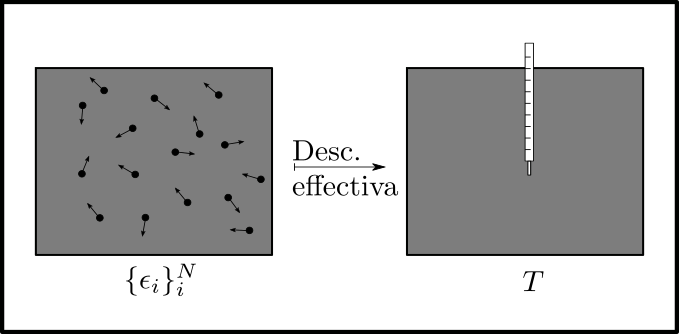
\includegraphics[width=0.6\linewidth]{chapter1/figures/CGT.png}
    \caption{Reducir las energías cinéticas individuales de $N$ partículas a un temperatura es un modelo de grano grueso}
    \label{fig:KtoT}
\end{figure}

En mecánica estadística se utiliza la estadística para pasar de una descripción fina a una gruesa, en la que cantidades arbitrariamente grandes de variables son sustituidas por distribuciones de probabilidad.

Los modelos de grano grueso son útiles porque permiten hacer predicciones sin tener que lidiar con cantidades de información que pueden ser no manejables, o simplemente no accesibles. Por esta razón, los modelos de grano grueso son comunes en física-química \cite{PhysChemI,PhysChemII,PhysChemIII} \acnote{revisar bien estos artículos}.


\subsection{Grano grueso en mecánica cuántica}

\acnote{Sección iterada, notas}

En el contexto de la mecánica cuántica, un modelo de grano grueso puede obtenerse trazando sobre un subsistema del sistema de interés. Es importante notar que el subsistema ignorado no es necesariamente una parte que puede ser separada del sistema, como en el caso de dos partículas, sino que puede representar otros grados de libertad del sistema que se deciden ignorar, por ejemplo, al describir un ión atrapado en una trampa magnetoóptica, una opción es ignorar los grados de libertad espaciales y quedarse solo con el espín total del ión \cite{Fox}. Ahora, la separación sistema-entorno no es siempre posible \cite{Macro-To-Micro}, por lo que nos limitamos a los casos en los que los grados de libertad ignorados pueden trazarse a través de la operación de traza parcial, como se discutió en la sección \ref{sec:Ch1PartialTrace}.

Un ejemplo sencillo de un modelo de grano grueso es el de un sistema de dos partículas, del cual únicamente nos importa una. En dicho caso, el modelo puede consistir en estudiar únicamente al operador de densidad reducido correspondiente a la partícula de nuestro interés. De forma general en el contexto de este trabajo, el modelo de grano grueso consiste en reducir la dimensión del sistema estudiado. En nuestro contexto, una aplicación de grano grueso $\Lambda$ es tal que manda a un operador de densidad $\varrho\in\densityspace{n}$ a algún otro operador de densidad $\rho\in\densityspace{m}$ con $m<n$. Esto es:
\begin{align}
    \mcF:\densityspace{n}\to \densityspace{m}, n>m\nonumber
\end{align}
\newpage
\chapter{La Asignación de Máxima Entropía y su evolución}

Con las bases asentadas, es posible pasar al estudio del problema propuesto por este trabajo: el estudio de la dinámica efectiva asociada a un modelo de grano grueso y a una aplicación se asignación.

Supongamos que estudiamos un sistema cuántico de varias partículas, que hemos logrado aislarlo de forma que evolucione como un sistema cuántico cerrado, y que conocemos a ciencia cierta la forma de la evolución seguida por el sistema.

En principio, asumiendo que somos capaces de realizar una tomografía de estado, parecería que no tendríamos ningún problema para conocer el estado del sistema a un tiempo arbitrario, pues tenemos acceso al estado inicial del sistema. Sin embargo, al comenzar a realizar las mediciones necesarias para llevar a cabo la tomografía, nos damos cuenta de que nuestra instrumentación no sólo no puede resolver todos los grados de libertad del sistema, sino que tiene una probabilidad no nula de fallar (de inducir ruido).

\ddnote*{Al no poder acceder a todos los grados de libertad del sistema}{Al no poder acceder a todas las dimensiones del sistema}, nuestra descripción es, efectivamente, un modelo de grano grueso. ¿Cómo podemos describir la evolución del sistema que estamos estudiando? ¿Cómo evoluciona el estado efectivo accesible?

En este capítulo describiremos matemáticamente la aplicación de grano grueso con la que se trabajará, luego se utilizará el Principio de Máxima Entropía para hallar el mejor \ddnote*{estimado qué?}{estimado} posible dada nuestra descripción efectiva, y finalmente se propondrá un modelo de la dinámica efectiva. La dinámica efectiva siendo la evolución que el experimentalista observaría.


\section{Un modelo de grano grueso y borroso}


Como se discutió previamente, es natural suponer que no siempre es posible disponer de toda la información sobre el \textit{estado} del sistema de interés. Esto ya sea por insuficiencia en la resolución de los aparatos de medición o por el inevitable error inherente a las herramientas de medición. Un prototipo sencillo de error consiste en el inducido por un aparato que no distingue diferentes conjuntos de partículas entre sí. El caso más simple corresponde a la permutación de dos partículas. Este intercambio accidental a la hora de la medición es una \textit{aplicación borrosa} \cite{FuzzyMeasurements}.

Para ilustrar lo anterior, considérese dicha aplicación borrosa sobre un sistema de dos partículas. Para simplificarlo un poco más, supongamos que cada partícula es un sistema de dos niveles, esto es, el sistema está compuesto por los qubits $A$ y $B$. El estado del sistema está caracterizado por un operador de densidad $\varrho_{AB} \in \mcS(\hilbert_2 \otimes \hilbert_2)$. La acción de la aplicación borrosa se escribe como sigue:
\begin{align*}
\mcF:&\mcS(\hilbert_2 \otimes \hilbert_2)\to \mcS(\hilbert_2 \otimes \hilbert_2)\nonumber\\
&\varrho \mapsto p\varrho+(1-p)S\varrho S,
\end{align*}
donde $0<p<1$ es la probabilidad con la que el aparato de medición identifica erróneamente a los dos subsistemas y $S$ es el operador de transposición de dos partículas (llamado operador SWAP), definido como 
\begin{equation*}
    S\ket{\psi}\otimes \ket{\phi}=\ket{\phi}\otimes \ket{\psi} \ \ \forall \ket{\psi},\ket{\phi}\in \hilbert_2.
\end{equation*}
El estado resultante, $\Fuzzy{\varrho_{AB}}=p\varrho_{AB}+(1-p)\varrho_{BA}$, es una mezcla estadística del estado accesible con un detector perfecto, $\varrho_{AB}$, y el estado donde los qubits tienen las etiquetas equivocadas, $\varrho_{BA}:=S\varrho_{AB} S$. Así, si quisieramos hallar el valor esperado del observable $\sigma_{3}\otimes\Id$ (el valor esperado de $\sigma_{z}$ en la primer partícula), encontraríamos:
\begin{equation*}
    \expval{\sigma_{3}\otimes\Id}_{\mcF}=(1-p)\expval{\sigma_{3}\otimes\Id}+p\expval{\Id\otimes\sigma_{3}}
\end{equation*}
donde por $\expval{A}_{\mcF}$ nos referimos al valor esperado con respecto al estado del sistema descrito a través de $\mcF$.

Es importante notar que, auque la aplicación borrosa modela el error asociado al aparato de medición, no constituye por si misma un modelo de grano grueso, pues conserva la dimensión del sistema: el aparato resuelve todos los grados de libertad.

Agreguemos al error por permutación la falta de resolución. Una posibilidad es que el instrumento detecte una partícula en donde en realidad haya dos, y aún más, que en un sistema de dos partículas, este sea capaz de medir únicamente observables asociados al primer subsistema. El estado observado sería, de acuerdo con la sección \ref{sec:PartialTrace}, la matriz de densidad reducida de la primera partícula. Matemáticamente, la composición del error y de la falta de resolución puede escribirse como
\begin{gather*}
    \mcC:\mcS(\hilbert_2 \otimes \hilbert_2)\to \mcS(\hilbert_2)\nonumber\\
    \rho_{AB} \mapsto p\rho_A+(1-p)\rho_B\rlap{,}
\end{gather*}
donde $\rho_A=\tr_B \rho_{AB}$ y $\rho_B=\tr_A \rho_{AB}$, es decir, las matrices de densidad reducidas de la partículas $A$ y $B$, respectivamente.


A diferencia de la aplicación borrosa, el modelo de grano grueso disminuye la dimensión del estado resultante. Además se puede mostrar que la ecuación anterior puede reescribirse en términos de la aplicación borrosa \cite{FuzzyMeasurements},
\begin{equation}\label{eq:CG}
\CG{\rho}=(\Tr_{B}\circ\mcF)[\rho].
\end{equation}
En este contexto, diferenciamos al estado ``microscópico'' o ``fino'', denotado por $\varrho\in \mcS(\hilbert_2\otimes\hilbert_2)$, y al estado ``macroscópico'', ``grueso'', o  ``efectivo'' denotado por $\rho\in \mcS(\hilbert_2)$, a través de la relación
\begin{equation*}
    \rho=\CG{\varrho}.
\end{equation*}
Es extremadamente importante notar que la expresión anterior no es invertible. Pueden existir una infinidad de estados $\varrho$ tales que su descripción gruesa coincida con $\rho$. Como ejemplo, supóngase que el estado efectivo está descrito por $\rho=\frac{1}{2}\Id$, el estado máximamente mezclado. Entonces cualquier sistema fino que se halle en un estado máximamente entrelazado será compatible con la descripción efectiva $\frac{1}{2}\Id$.

Pues bien, como se ha asumido que conocemos la evolución unitaria subyacente, requerimos asignar a $\rho$ un estado microscópico que cumpla con todas las restricciones impuestas por nuestras mediciones. Asumiremos que dicho estado asignado es el que experimenta la evolución. 

\section{Construcción del estado de máxima entropía}

\acnote{Párrafo iterado: solo notas.}

Sea $\rho_{\ef}\in\mcS(\hilbert_{2})$ el estado grueso accesible al observador, y sea $\{A_{j}\}_{j}$ con $A_{j}\in\obspace{2}$ un conjunto de observables tomográficamente completo.
Si $\rho_{\ef}$ es un estado grueso correspondiente a un estado fino $\varrho\in\mcS(\hilbert_{2}^{\otimes n})$, de acuerdo con lo discutido en el capítulo anterior, podemos asignar a $\rho_{\ef}$ un estado microscópico que maximice la entropía de Von Neumann que satisfaga las restricciones $\expval{A_{j}}=\Tr(\rho_{\ef} A_{j})$.
Escójase ${A_{i}}={\pauli{i}}$, las matrices de Pauli, y la aplicación de grano grueso desarrollada en la sección anterior, aquella del grano grueso y borroso dada por (\ref{eq:CG}). Los valores esperados de los operadores se traducen como las componentes del vector de Bloch del operador $\rho_{\ef}$. Las restricciones a las que se ve sujeto el operador $\varrho_{\max}$ son
\begin{equation}
    r_{j}=\Tr[\pauli{j}\rho_{\ef}]\nonumber
\end{equation}
\acnote{Párrafo iterado: notación}

Aquí hay un problema: el estado que maximiza la entropía pertenece al espacio $\densityspace{2^{n}}$, mientras que las restricciones están definidas para un operador de densidad en $\densityspace{2}$. Entonces, ¿cómo se traducen dichas restricciones en el nivel microscópico? Naturalmente, esto dependerá de la relación entre el estado efectivo $rho_{\ef}$ y el estado subyacente $\varrho$. Esto es, el estado de máxima entropía depende de la aplicación de grano grueso. Sustituyendo la relación entre algún estado microscópico compatible $\varrho$ y el estado efectivo $\rho_{\ef}$ en la ecuación anterior, y manipulando un poco se halla que
\begin{align}
    r_{j}&=\Tr[\sigma_{j}\CG{\varrho}]\nonumber\\
    &=\Tr[\sigma_{j}\Tr_{\overline{1}}\qty(p_{1}\varrho+\sum_{k=2}^{n}p_{k}S_{1,k}\varrho S_{1,k}^{\dagger})]\nonumber\\
    &=\Tr[\sigma_{j}\otimes\Id_{2^{n-1}}\qty(p_{1}\varrho+\sum_{k=2}^{n}p_{k}S_{1,k}\varrho S_{1,k}^{\dagger})]\nonumber\\
    &=\Tr[\qty(p_{1}(\sigma_{j}\otimes\Id_{2^{n-1}})+\sum_{k=2}^{n}p_{k}S_{1,k}^{\dagger}(\sigma_{j}\otimes\Id_{2^{n-1}})S_{1,k})\varrho]\nonumber\\
    &=\Tr[\qty(p_{1}(\sigma_{j}\otimes\Id_{2^{n-1}})+\sum_{k=2}^{n}p_{k}(\Id_{2^{k-1}}\otimes\sigma_{j}\otimes\Id_{2^{n-k}}))\varrho]\nonumber\\
    &=\Tr[\qty(\sum_{k=1}^{n}p_{k}(\Id_{2^{k-1}}\otimes\sigma_{j}\otimes\Id_{2^{n-k}}))\varrho]\nonumber.
\end{align}
Definiendo
\begin{equation}\label{eq:GhatNM}
    \hat{G}_{j}=\sum_{k=1}^{n}p_{k}(\Id_{2^{k-1}}\otimes\sigma_{j}\otimes\Id_{2^{n-k}}),
\end{equation}
las restricciones se pueden esribir como
\begin{equation}\label{eq:MaxEntRestrictions}
    r_{j}=\Tr[\hat{G}_{j}\varrho].
\end{equation}
Estas restricciones ya se hallan en términos de observables y un operador de densidad que actúan sobre $\hilbert_{2^{n}}$. Entonces se utilizan multiplicadores de Lagrange para obtener el estado de maximiza la entropía. De acuerdo con la ecuación (\ref{eq:GeneralMaxEnt}), el estado de máxima entropía compatible con (\ref{eq:MaxEntRestrictions}) es
\begin{equation}\label{eq:MaxEntLagMult}
    \varrho_{\max}=\frac{1}{Z}e^{\sum_{j}\lambda_{j}\hat{G}_{j}}.
\end{equation}
Si se sustituye a $\varrho_{\max}$ en las ecuaciones (\ref{eq:MaxEntRestrictions}) (cosa nada recomendable), se obtienen las relaciones entre los multiplicadores de Lagrange y los valores esperados de los observables utilizados para la tomografía. Si se escribe $\lambda=\sqrt{\lambda_{1}^{2}+\lambda_{2}^{2}+\lambda_{3}^{2}}$, los resultados son
\begin{align}\label{eq:MaxEntExpVals}
    \begin{split}
    \expval{\pauli{1}}&=\lambda_{1}\rfroml(\lambda),\\
    \expval{\pauli{2}}&=\lambda_{2}\rfroml(\lambda),\\
    \expval{\pauli{3}}&=\lambda_{3}\rfroml(\lambda),
    \end{split}
\end{align}
donde $\rfroml(\lambda)$ es una función biyectiva de $\lambda$, y cuya forma será derivada en la siguiente sección de una forma que requiere muchas menos cuentas. Idealmente, la ecuación (\ref{eq:MaxEntLagMult}) está en términos de los valores de expectación $r_{i}=\Tr(\sigma_{i}\rho_{\ef})$, y no de los multiplicadores de Lagrange. Aunque no es posible despejar a los multiplicadores de Lagrange de las ecuaciones de manera algebráica, la naturaleza de $\rfroml(\lambda)$ nos permite asegurar que las relaciones son uno a uno y que tienen inversa.

A partir de este momento, cada vez que se hable del \textit{estado de máxima entropía}, se entiende que se hace referencia al estado dado por la ecuación (\ref{eq:MaxEntLagMult}). Esto es, al estado de máxima entropía que es compatible con un estado efectivo inducido por nuestro modelo de grano grueso particular.
\section{Análisis del estado de máxima entropía}

\subsection{Factorizabilidad}

Nótese que el argumento de la exponencial en la ecuación (\ref{eq:MaxEntLagMult}) está conformado por operadores que conmutan entre sí:
\begin{equation}
    \sum_{j=1}^{3}\lambda_{j}\hat{G}_{j}=\sum_{j=1}^{3}\lambda_{j}\sum_{k=1}^{n}p_{k}(\Id_{2^{k-1}}\otimes\sigma_{j}\otimes\Id_{2^{n-k}}).\nonumber
\end{equation}
Esto significa que el estado de máxima entropía es factorizable y tiene exactamente $n$ factores. Explícitamente,
\begin{equation}\label{eq:MaxEntSeparable}
    \varrho_{\max}=\Motimes_{k=1}^{n}\frac{1}{Z_{k}}\text{exp}\qty(p_{k}\sum_{j=1}^{3}\lambda_{j}\sigma_{j}).
\end{equation}

¿Por qué el estado de máxima entropía resulta ser factorizable respecto a todas las partículas del sistema microscópico? Para responder a esta pregunta, primero hace falta ver que la información accesible al experimentalista no incluye las correlaciones entre los subsistemas. Para ver esto, considérese la parametrización de Bloch de un estado fino $\varrho\in\mcL(sa\hilbert_{4})$ como propuesta en (\ref{eq:BlochParametrization4}). Esto es,
\begin{align}\label{}
    \varrho=\frac{1}{4}\sum_{j,k=0}^{3}\gamma_{jk}\sigma_{i}\otimes \sigma_{k} & & \text{con} & & \gamma_{jk}=\Tr(\sigma_{j}\otimes \sigma_{k}\varrho).\nonumber
\end{align}
De acuerdo con la ecuación (\ref{eq:Ch1PartialTrace}) las matrices de densidad reducidas de $\varrho$ en términos de los parámetros $\gamma_{jk}$ son
\begin{align}
    \rho_{1}=\frac{1}{2}\sum_{j=0}^{3}\gamma_{0j}\pauli{j} & & \text{y} & & \rho_{2}=\frac{1}{2}\sum_{j=0}^{3}\gamma_{j0}\pauli{j}.\nonumber
\end{align}
La matriz de densidad reducida contiene la información estadística de dicho subsistema. Esto significa que las correlaciones entre los subsistemas están contenidas en los elementos $\gamma_{jk}$ tales que $j,k\neq 0$ (los elementos no presentes en las matrices de densidad reducidas). Ahora, la acción de la aplicación de grano grueso sobre la matriz de densidad es justamente
\begin{align}
    \CG{\varrho}&=\Tr_{2}\qty[(p \varrho + (1-p)S\varrho S]\nonumber\\
    &=p\rho_{1}+(1-p)\rho_{2}\nonumber\\
    &=\frac{1}{2}\qty(\Id+\sum_{k=1}^{3}(p\gamma_{k0}+(1-p)\gamma_{0k})\sigma_{k}).\nonumber
\end{align}
¡El estado efectivo no contiene información sobre las correlaciones del estado subyacente! Una consecuencia de esto es que todos los estados pertenecientes a un conjunto de estados microscópicos cuyas matrices de densidad reducidas coinciden tienen la misma imagen bajo la aplicación de grano grueso. Matemáticamente, si se tienen dos estados microscópicos, $\varrho_{A}$ y $\varrho_{B}$, y estos estados cumplen que
\begin{align}
    \Tr_{2}[\varrho_{A}]=\rho_{1} & & \Tr_{1}[\varrho_{A}]=\rho_{2} & & \text{y} & &\Tr_{2}[\varrho_{B}]=\rho_{1} & & \Tr_{1}[\varrho_{B}]=\rho_{2},\nonumber
\end{align}
entonces
\begin{align}
    \CG{\varrho_{A}}=\CG{\varrho_{B}}.\nonumber
\end{align}
Como el estado de máxima entropía respeta el hecho de que no tenemos acceso a las correlaciones, todas ellas, contenidas en los elementos $\gamma_{jk}$ tales que $j,k\neq 0$ se hacen cero \footnote{Es importante señalar que esto no implica que las entradas $\gamma_{jk}$ tales que $j,k\neq 0$ de un estado de máxima entropía $\varrho_{\max}\in\mcL(\hilbert_{4})$ sean nulas (basta con desarrollar la expresión (\ref{eq:MaxEntSeparable}) para ver que no es así), si no que las correlaciones contenidas en dichos elementos son nulas, esto es $\gamma_{jk}=\gamma_{0k}\gamma_{j0}$.}. 


\acnote{Párrafo iterado: notas}

La expresión (\ref{eq:MaxEntSeparable}) es un producto tensorial de $n$ operadores de densidad, a los que denotaremos como $\rho_{j}$, con $\rho_{j}\in\mcL(\hilbert_{2})$. Aún más, nótese que si definimos al vector unitario $\hat{\lambda}$ a través de
\begin{equation}
    \hat{\lambda}_{i}=\frac{\lambda_{i}}{\lambda},\nonumber
\end{equation}
con $\lambda$ dada por la ecuación (\ref{eq:Ch2LagrangeNorm}), entonces todos los factores pueden reescribirse como la exponencial real de $\lambda(\paulivec{\lambda})$ pesado por un factor probabilístico. Ahora, en virtud de la relación (\ref{ap:PauliRealExp}) hallamos
\begin{equation}
    \rho_{j}=\frac{1}{Z_{j}}\qty(\Id\cosh{p_{j}\lambda}+\paulivec{\lambda}\sinh{p_{j}\lambda}).\nonumber
\end{equation}
Para que las matrices reducidas representen estados válidos, las funciones de partición $Z_{j}$ deben valer
\begin{equation}
    Z_{j}=2\cosh{p_{j}\lambda}.\nonumber
\end{equation}
Las matrices de densidad reducidas del estado de máxima entropía tienen la forma
\begin{equation}\label{eq:rhoArhoB}
    \rho_{j}=\frac{1}{2}\qty(\Id+\paulivec{\lambda}\tanh{p_{j}\lambda}).
\end{equation}

\subsection{La relación entre multiplicadores y mediciones}

\acnote{Mediciones? Promedios?}

\acnote{Párrafo iterado: notas}

El problema de la ecuación (\ref{eq:MaxEntSeparable}) es que el estado de máxima entropía está en términos de los multiplicadores de Lagrange, en lugar de cantidades con un significado físico claro. Si por alguna razón tuviéramos que resignarnos a trabajar con el estado en términos de los $\lambda_{i}$, será necesario conocer la expresión del estado macroscópico. Para hallarla, basta con pasar al estado de máxima entropía por la aplicación de grano grueso. Por construcción 
\begin{equation}
    \rho_{\ef}=\CG{\varrho_{\max}}=\sum_{j=1}^{n}p_{j}\rho_{j}.\nonumber
\end{equation}
Sustituyendo las fórmulas de $\rho_{j}$, obtenemos al estado grueso en términos de los multiplicadores de Lagrange.
\begin{equation}\label{eq:CG(MaxEnt)}
    \rho_{\ef}=\frac{1}{2}\qty[\Id+(\paulivec{\lambda})\qty(\sum_{j=1}^{n}p_{j}\tanh(p_{j}\lambda))].
\end{equation}
Pues bien, el estado efectivo tiene su propia parametrización de Bloch. Sea $\vec{r}_{\ef}$ el vector de Bloch de la partícula efectiva. Entonces es claro que
\begin{align}
    r_{\ef}=\sum_{j=1}^{n}p_{j}\tanh(p_{j}\lambda) && \text{y} && \hat{r}_{\ef}=\hat{\lambda},\nonumber
\end{align}
que no son más que la norma y dirección del vector de Bloch del estado efectivo en términos de $\lambda$. De esta manera deducimos la relación entre los promedios de las observables a nivel grueso $\expval{\pauli{j}}=r_{\ef}(\hat{r}_{\ef})_{j}$ y los multiplicadores de Lagrange introducidos para la maximización de la entropía, y es
\begin{equation}
    \expval{\pauli{j}}=\frac{\lambda_{j}}{\lambda}\rfroml(\lambda).
\end{equation}
donde $\rfroml(\lambda)$ es la función que aparece en las ecuaciones (\ref{eq:MaxEntExpVals}),
\begin{equation}\label{eq:r(lambda)}
    \rfroml(\lambda)=\sum_{j=1}^{n}p_{j}\tanh(p_{j}\lambda)
\end{equation}
Ahora, la ecuación (\ref{eq:r(lambda)}), fijadas $p_{j}$, es una suma de $n$ funciones inyectivas, y como tal, es inyectiva también. Esto significa que existe la función inversa. La figura \ref{fig:r(lambda)} muestra la forma de $\rfroml(\lambda)$ para valores selectos de $p_{1}$ en el caso en que $n=2$. Después de una breve inspección de (\ref{eq:r(lambda)}) se concluye que los estados puros corresponden al caso límite $\lambda\rightarrow+\infty$.
Cada multiplicador de Lagrange queda determinado de forma única a través de cantidades experimentales según 
\begin{equation}
    \lambda_{i}=\rfroml^{-1}(r_{\ef}) \frac{\expval{\pauli{i}}}{r_{\ef}},
\end{equation}
y, por supuesto,
\begin{equation}
    \lambda=\rfroml^{-1}(r_{\ef})\nonumber
\end{equation}
Aunque siempre exista, no es posible hallar una expresión de $\rfroml^{-1}$ para cualquier valor de $p$ debido a que la ecuación (\ref{eq:r(lambda)}) es una ecuación trascendental. Por esto, para escribir al estado de máxima entropía como una función de cantidades medibles, nos tendremos que conformar con llamar a $\rfroml^{-1}$ de manera explícita.
\begin{figure}[ht!]
    \centering
    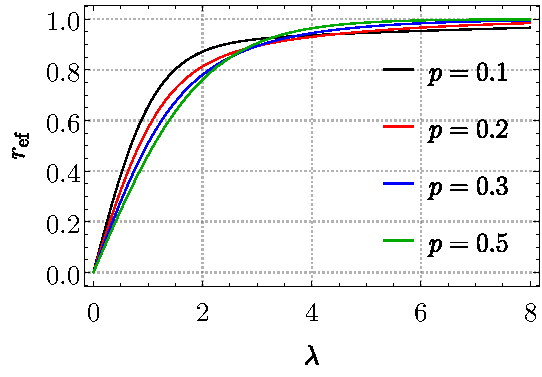
\includegraphics[width=0.5\linewidth]{chapter3/figures/r(lambda).pdf}
    \caption{$r_{\ef}$ como función de $\lambda$ para diferentes valores de $p_{1}$ en el caso en que $n=2$.}
    \label{fig:r(lambda)}
\end{figure}

\subsection{Otra expresión del estado de máxima entropía}

\acnote{Al final nunca usé esto, ¿se queda?}

La ecuación (\ref{eq:MaxEntSeparable}) sugiere que el estado de máxima entropía puede expresarse como producto tensorial de potencias de un mismo estado. En efecto, dado un real $q$ y una matriz cuadrada $A$, la potenciación $A^{q}$ puede escribirse como $e^{q \ln A}$. Como las matrices $e^{\sum_{i}\lambda_{i}\pauli{i}}$ son positivas semidefinidas, su logaritmo es único en el caso de no ser degenerado, y en caso de degeneración, basta con tomar la rama principal \cite{log1,Davalos2019}. Entonces,
\begin{equation}
    \varrho_{\max}=\Motimes_{j=1}^{n}\frac{1}{Z_{j}}e^{p_{j}\sum_{k}\lambda_{k}\pauli{k}}=\Motimes_{j=1}^{n}\frac{1}{Z_{j}}\qty(e^{\sum_{k}\lambda_{k}\pauli{k}})^{p_{j}}.\nonumber
\end{equation}
En virtud de (\ref*{ap:PauliRealExp}), se cumple que
\begin{align}
  \varrho_{\max}=&\Motimes_{j=1}^{n}\frac{\qty(\cosh{\lambda}(\Id+\tanh{\lambda}(\paulivec{r_{\rho}})))^{p_{j}}}{\Tr[\qty(\cosh{\lambda}(\Id+\tanh{\lambda}(\paulivec{r_{\rho}})))^{p_{j}}]}\nonumber\\
  =&\Motimes_{j=1}^{n}\frac{\qty(\Id+\tanh{\lambda}(\paulivec{r_{\rho}}))^{p_{j}}}{\Tr[\qty(\Id+\tanh{\lambda}(\paulivec{r_{\rho}}))^{p_{j}}]}.\nonumber
\end{align}
Definimos
\begin{equation}\label{eq:Xi}
  \Xi_{\max}=\frac{1}{2}(\Id+\tanh{\lambda}(\paulivec{r_{\rho}})),
\end{equation}
de tal manera que 
\begin{equation}\label{eq:MaxEntSeparablePower}
  \varrho_{\max}=\Motimes_{j=1}^{n}\frac{(\Xi_{\max})^{p_{j}}}{\Tr[ (\Xi_{\max})^{p_{j}}]}.
\end{equation}

\subsection{La asignación de máxima entropía}

El estado de máxima entropía nos otorga una herramienta de asignación para los estados efectivos. Después de todo, requerimos de una asignación razonable que pueda ser propagada según la dinámica microscópica conocida. Sea $\rho_{\ef}\in\densityspace{2}$ un estado efectivo, entonces definimos a la aplicación de asignación de máxima entropía como
\begin{equation}\label{eq:MaxEntAss}
    \begin{gathered}
        \mcA_{\mcC}^{\max}:\densityspace{2}\rightarrow\densityspace{2^{n}}\nonumber\\
        \rho_{\ef} \mapsto \Motimes_{j=1}^{n}\frac{1}{Z_{j}}\text{exp}\qty(p_{j}\sum_{k=1}^{3}\lambda_{k}\sigma_{k}).
    \end{gathered}
\end{equation}
donde la dependencia de la asignación en el modelo de grano grueso se indica mediante un subíndice, $\mcC$. Nótese que según los valores que puedan tomar las diferentes probabilidades $p_{j}$, el estado asignado tendrá diferentes propiedades. Nos concentramos en dos casos particulares. El primero corresponde a $p_{1}=1$. En este caso se eliminan los términos de error, y el estado de máxima entropía es simplemente
\begin{equation}\label{eq:PreferentialAss}
    \varrho_{\max}=\rho_{\ef}\otimes\Id^{2^{n-1}},
\end{equation}
Nótese que la aplicación de asignación se vuelve lineal si no hay error de medición. Esto debe verse como un caso límite. Este trabajo estudiará $p_{1}\rightarrow 1$ como el escenario en el que la probabilidad de detectar la partícula equivocada es pequeña. De acuerdo con esto, se le llamará  \textit{regimen de partícula preferencial}.

Ahora, si por otro lado, $p_{j}=\frac{1}{n}\forall j$, entonces el estado de máxima entropía es
\begin{equation}
    \varrho_{\max}=\qty[\frac{1}{Z}\text{exp}\qty(\frac{1}{n}\sum_{k=1}^{3}\lambda_{k}\sigma_{k})]^{\otimes n}=(\rho')^{\otimes n}.\nonumber
\end{equation}
Si se pasa este estado por la aplicación de grano grueso correspondiente el resultado es 
\begin{equation}
    \mcC[\varrho_{\max}]=\sum_{j=1}^{n}\frac{1}{n}\rho'=\rho',\nonumber
\end{equation}
de  lo que se concluye que
\begin{equation*}
    \rho'=\rho_{\ef},
\end{equation*}
y que por lo tanto el estado asignado es simplemente
\begin{equation}\label{eq:BoltzmannAss}
    \mcA_{\mcC}^{\max}(\rho_{\ef})=\rho_{\ef}^{\otimes n}.
\end{equation}
Así, si $p_{j}=\frac{1}{n}\forall j$, la asignación de máxima entropía resulta en un estado factorizable de $n$ partículas idénticas. A este caso se le llamará \textit{régimen imparcial}.



Ahora supóngase que $\varrho$ es un estado microscópico compatible con un estado efectivo puro $\rho_{\ef}=\dyad{\psi}$, y que $p_{j}\neq 0\,\forall\,j$. Entonces, por (\ref{eq:MaxEntSeparable}) se cumple que
\begin{equation}
    \rho_{ef}=\sum_{k=1}^{n}p_{k}\varrho_{k},\nonumber
\end{equation}
donde $\varrho_{k}\in\densityspace{2}$ es la $k$-ésima traza parcial de $\varrho$. Como se mencionó en la sección \ref{subsec:ch2_purity}, un estado puro es un punto extremo del conjunto de estados, así que la ecuación anterior solo se puede cumplir si $\varrho_{k}=\dyad{\psi}\,\forall\,k$.  Si cada traza parcial de $\varrho$ es igual al estado puro $\rho_{\ef}$ se sigue que
\begin{equation}\label{eq:PureEffectiveState}
    \varrho=\left(\dyad{\psi}\right)^{\otimes n}.
\end{equation}
Nótese que para obtener (\ref{eq:PureEffectiveState}) no se hizo ninguna suposición sobre la aplicación de asignación. Lo que se acaba de demostrar es que, dado que todas las trazas parciales participen en la aplicación de grano grueso, el único estado microscópico compatible con un estado efectivo puro es el $n$-producto de dicho estado. El estado (\ref{eq:PureEffectiveState}) es un estado coherente de espín~\cite{klimovbook}~\footnote{Los estados coherentes de $n$ espines $1/2$ consisten en estados puros donde todas las partículas están ``alineadas'' en la misma dirección en la esfera de Bloch. Es decir, simplemente se tiene que $\ket{\psi_\text{coh}}=\ket\psi^{\otimes n}$, en virtud de que estos estados saturan la relaciones de incertidumbre de espín.}.

\section{Construcción de la dinámica}\label{sec:ch2dycon}

Ahora que hemos establecido que usaremos como modelo de grano grueso uno que incluye tanto problemas de resolución como errores de permutación, y que hemos contruído nuestra aplicación de asignación a través del Principio de Máxima Entropía, podemos preguntarnos sobre la evolución del sistema efectivo, la ``dinámica gruesa'', denotada como $\Gamma_t$. La dinámica efectiva es un mapa dinámico que corresponde a la evolución observada por un experimentalista. Dado un estado efectivo inicial $\rho_{\ef}(0)$,
\begin{gather}
\Gamma_{t}:\mcS(\hilbert_2)\rightarrow \mcS(\hilbert_2)\nonumber\\
\rho_{\ef}(0) \mapsto \rho_{\ef}(t)\rlap{.}\nonumber
\end{gather}
Debido que asumimos que el estado que se propaga debido a la evolución subyacente es justamente el estado de máxima entropía, a la dinámica gruesa la definimos como la composición
\begin{equation}
\Gamma_t:=\mcC \circ \mcV_t \circ \mcA_\mcC.\nonumber
\end{equation}
Donde $\mcA_\mcC$ denota a la aplicación que asigna un estado microscópico $\varrho$ al estado efectivo $\rho_{\ef}$. A la aplicación de asignación desarrollada previamente la denotaremos por medio de $\mcA_{\mcC}^{\max}$. El siguiente diagrama ilustra la ecuación anterior,
\[\begin{tikzcd}[arrows={<-|}]
    \rho_{\ef}(0)  & \rho_{\ef}(t) \arrow{l}{\Gamma_{t}} \arrow{d}{\mcC}\\
\varrho(0) \arrow{u}{\mcA_{\mcC}^{\max}} & \varrho(t). \arrow{l}{\mcV_{t}}
\end{tikzcd}
\]
En el siguiente capítulo se analizarán dinámicas efectivas generadas por diferentes dinámicas subyacentes. Si se asume que el sistema conformado por las partículas es cerrado, entonces la evolución $\mcV_{t}$ será unitaria, generada por un hamiltoniano $H$. Algunos ejemplos de dinámicas subyacentes no unitarias son los canales de ruido usuales, como el canal de despolarización, el canal de amortiguamiento de amplitud, o el canal de amortiguamiento de fase.

Nótese que, a diferencia de los mapas dinámicos usualmente estudiados en teoría de sistemas cuánticos abiertos, la dinámica efectiva $\Gamma_{t}$ no tiene por qué ser lineal (sí debe, por supuesto, mandar estados en estados), debido a que uno de los elementos de la composición que la originan no es lineal: la aplicación de asignación. El estudio de las particularidades de algunas de estas dinámicas efectivas es el foco de este trabajo.

Reconociendo que la asignación de máxima entropía no es la única asignación compatible con un conjunto de aplicación de grano grueso y estado inicial efectivo, ¿es justificable usar al estado de máxima entropía? Previamente demostramos que en nuestro caso particular, este resulta ser separable, y aunque en el caso estacionario esto no afecta, las correlaciones, que se anulan en esta asignación, sí afectan la forma en que un sistema evoluciona.

Algo que queda en claro de esto es que el estado de máxima entropía es completamente dependiente de los observables que se usen en su construcción. Después de todo, la maximización de la entropía se restringe de acuerdo a las observaciones experimentales, así que estados de máxima entropía que cumplan un conjunto particular de restricciones no tienen por qué (y probablemente no lo harán) satisfacer un conjunto diferente de restricciones, un conjunto mediante el cual se construiría un estado de máxima entropía diferente. Esto tiene la siguiente consecuencia: el estado de máxima entropía compatible con un estado evolucionado a través de una dinámica efectiva obtenida de un estado de máxima entropía compatible con un estado efectivo inicial, no tiene por qué ser igual al estado de máxima entropía inicial evolucionado. Esto es, no tiene por que cumplirse que
\begin{equation}
    (\mcU_{t}\circ\mcA_\mcC)(\rho) = (\mcA_\mcC\circ\mcC \circ \mcU_t \circ \mcA_\mcC)(\rho).\nonumber
\end{equation}
Y la razón de esto es que
\begin{equation}
    \mcA_\mcC\neq\mcC^{-1}.\nonumber
\end{equation}


\newpage

\chapter{Dinámica efectiva}\label{sec:chapter3}

\acnote{Párrafo iterado: notas}

En este capítulo se estudiarán las dinámicas efectivas inducidas por diferentes tipos de dinámicas microscópicas. Primero, motivados por el hecho de que el estado de máxima entropía es factorizable, se analizarán dinámicas generadas por hamiltonianos que no tengan partes de interacción. Luego se estudiarán compuertas de dos qubits bien conocidas en cómputo cuántico: la compuerta SWAP y la compuerta CNOT (que si presentan interacciones entre las dos partículas). Finalmente se profundizará en dinámicas más específicas, como una cadena de partículas con interacción Ising, así como evoluciones no unitarias, como el canal de despolarización, el canal de amortiguamiento de amplitud, entre otras.

\section{Dinámicas locales}

En la sección \ref{sec:Ch1PartialTrace} se habló de estados separables como aquellos estados que, descritos por un operador de densidad $\rho\in\densityspace{n}$, tienen la forma
\begin{equation}
    \rho=\rho_{A}\otimes\rho_{B},\nonumber
\end{equation}
donde $\rho_{A}\in\densityspace{m}$, $\rho_{B}\in\densityspace{l}$ y $l+m=n$. Siguiendo esta línea de pensamiento, con \textit{dinámicas factorizables} nos referimos a dinámicas unitarias generadas por hamiltonianos que no contienen un término de interacción (que en el caso de dos partículas son hamiltonianos de la forma $\mcH=H_{1}\otimes\Id+\Id\otimes H_{2}$), y que por lo mismo son descritas por operadores $\mcU\in\unitaryspace{n}$ del tipo
\begin{equation}
    \mcU=U_{A}\otimes U_{B}.\nonumber
\end{equation}
De nuevo, $U_{A}\in\unitaryspace{m}$, $U_{B}\in\unitaryspace{l}$ y $l+m=n$. Los operadores separables están compuestos por operadores que actúan de forma independiente sobre diferentes subsistemas del sistema en cuestión. En el caso de un sistema compuesto por dos subsistemas de dos niveles, el operador separable está compuesto por dos unitarias que actúan sobre $\hilbert_{2}$. Como el estado de máxima entropía resulta ser separable, las dinámicas separables son una muy buena primera forma de aplicar el formalismo descrito en las secciones anteriores.

Considérese la aplicación de grano grueso de $n$ a $1$ partículas definida según (\ref{eq:CG}), un estado efectivo $\rho_{\ef}\in\densityspace{2}$ y la aplicación de máxima entropía compatible dada por (\ref{eq:MaxEntAss}). Si la evolución microscópica es factorizable entonces es generada por un hamiltoniano de la forma
\begin{equation}
    \mcH=\sum_{k=1}^{n}\omega_{k}\Id_{2^{k-1}}\otimes H_{k} \otimes \Id_{2^{n-k}},\nonumber
\end{equation}
siendo la unitaria 
\begin{equation}\label{eq:NFactorUnitaries}
    \mcU_{t}=\Motimes_{k=1}^{n}\text{exp}\qty(-\rmi\omega_{k}H_{k}t)=\Motimes_{k=1}^{n} U_{k}(t).
\end{equation}
A partir de este momento, para hacer más limpia la lectura de este documento se omitirán los productos tensoriales con operadores identidad. El subsistema sobre el que actúe un operador será denotado por un subíndice, de tal manera que el hamiltoniano previamente definido queda
\begin{equation}
    \mcH=\sum_{k=1}^{n}\omega_{k}H_{k}.\nonumber
\end{equation}


\subsection{Caso general}

Si se considera una evolución unitaria de la forma (\ref{eq:NFactorUnitaries}), y se propaga al estado obtenido de la aplicación de máxima entropía, el estado evolucionado es
\begin{equation}
    \varrho_{\max}(t)=\Motimes_{k=1}^{n}\frac{1}{Z_{k}}U_{k}(t) e^{\qty(p_{k}\sum_{j}\lambda_{j}\pauli{j})} (U_{k}(t))^{\dag}\nonumber
\end{equation}
El estado efectivo evolucionado en términos de los multiplicadores de Lagrange queda
\begin{equation}\label{eq:SeparableEvolution}
    \Gamma_{t}(\rho_{\ef})=\sum_{k=1}^{n}p_{k} U_{k}(t) \rho_{k} (U_{k}(t))^{\dag}.
\end{equation}
donde $\rho_{k}=\frac{1}{Z_{k}}e^{\qty(p_{k}\sum_{j}\lambda_{j}\pauli{j})}$. 

Por supuesto, esta expresión puede expandirse en términos de exponenciales o de funciones hiperbólicas del vector de Bloch del estado efectivo inicial, $\vec{r}_{\ef}$. Haciendo esto se obtiene una expresión para el valor esperado de $\pauli{j}$ a un tiempo $t$,
\begin{equation}\label{eq:SeparableEvolutionExpVal}
    \expval{\pauli{i}(t)}=\frac{1}{2}\sum_{k=1}^{n}p_{k}\tanh(p_{k}\lambda)\Tr[\pauli{j}U_{k}(t) (\hat{r}_{\ef}\cdot\vec{\sigma}) (U_{k}(t))^{\dag}]
\end{equation}
Si se piensa en el caso en que $p_{1}>p_{j}\,\forall j\neq 1$, separar la contribución del sistema de interés,
\begin{align}
    \expval{\pauli{j}(t)}=&\frac{1}{2}p_{1}\tanh(p_{1}\lambda)\Tr[\pauli{j}U_{1}(t) (\hat{r}_{\ef}\cdot\vec{\sigma}) (U_{1}(t))^{\dag}]\nonumber\\
    &+\frac{1}{2}\sum_{k=2}^{n}p_{k}\tanh(p_{k}\lambda)\Tr[\pauli{j}U_{k}(t) (\hat{r}_{\ef}\cdot\vec{\sigma}) (U_{k}(t))^{\dag}]\nonumber,
\end{align}
permite reconocer dos términos: uno asociado a la evolución \textit{sin error} de nuestro sistema, descrita por el operador unitario $U_{1}(t)$, y un término de ruido. La acción de este término dependerá tanto de la naturaleza de las evoluciones locales del entorno, como del número de partículas en este.


Por otro lado, en el caso en el que no hay partícula prioritaria, \ie ($p_{j}=\frac{1}{n}\forall j$), la relación entre la magnitud del vector de Bloch del estado efectivo y los multiplicadores de Lagrange es $\lambda=n\tanh^{-1}(r)$. Esto significa que la expresión del valor esperado de $\sigma_{j}$ a un tiempo $t$ es
\begin{equation}
    \expval{\pauli{j}(t)}=\frac{1}{2n}\sum_{k=1}^{n}\Tr[\pauli{j}U_{k}(t) (\vec{r}_{\ef}\cdot\vec{\sigma}) (U_{k}(t))^{\dag}],\nonumber
\end{equation}
que no es más que una combinación lineal de las mismas componentes evolucionadas de formas diferentes.
\subsection{Ejemplos particulares}

\subsubsection{Dinámica simétrica}

Comenzamos con el caso en el que la dinámica separable simétrica, esto es, de una unitaria $\mcU\in\unitaryspace{2^{n}}$ de la forma
\begin{equation}
    \mcU_{t}=\Motimes_{k=1}^{n}U(t),\nonumber
\end{equation}
donde $U(t)\in\unitaryspace{2}$. Se aplica la evolución al estado de máxima entropía compatible con un conjunto de observables tomográficamente completos en $\hilbert_{2}$ y se propaga al estado con la unitaria subyacente, para luego pasarlo por la aplicación de grano grueso y recuperar el estado efectivo evolucionado. Este caso es quizá el más sencillo, pues la simetría de la unitaria permite factorizarla:
\begin{align}
\mcC\qty[\Motimes_{k=1}^{n}U(t) \rho_{k} (U(t))^{\dag}]&=\sum_{k=1}^{n}p_{k} U(t) \rho_{k} (U(t))^{\dag}\nonumber \\
&=U(t)\qty(\sum_{k=1}^{n}p_{k} \rho_{k}) (U(t))^{\dag}\nonumber\\
&=U(t)\rho_{\ef}(U(t))^{\dag}.\nonumber
\end{align}
La dinámica efectiva tiene la forma
\begin{equation}
    \Gamma_{t}(\rho_{\ef})=U(t)\rho_{\ef}(U(t))^{\dag}.\nonumber
\end{equation}
Este resultado es natural. No solo no hay interacción entre los diferentes subsistemas, significando esto que no se \textit{filtra} ningún tipo de información entre la partícula de interés y el resto, sino que cada parte evoluciona de manera idéntica: bajo la aplicación de grano grueso, lo que se observa es una combinación de $n$ entidades idénticas evolucionando de la misma forma.

\subsubsection{Particulas no preferenciales invariantes}

Centrémonos, momentáneamente, en el régimen $p_{1}>p_{j}\,\forall j\neq 1$. Asúmase que la probabilidad de detectar a la $k$-ésima partícula es la misma para todas excepto la primera. Entonces
\begin{equation}
    p_{k}=\frac{(1-p_{1})}{n-1}\text{ }\forall k\neq 1.\nonumber
\end{equation}
El estado de máxima entropía compatible con un estado efectivo $\rho_{\ef}$ es
\begin{equation}
    \varrho_{\max}=\rho_{1}\otimes\qty(\Motimes_{k=2}^{n}\frac{1}{Z_{k}}e^{\frac{(1-p_{1})}{n-1}\sum_{j}\lambda_{j}\pauli{j}}),\nonumber
\end{equation}
donde, para todo $k$ se cumple que
\begin{equation}
    \frac{1}{Z_{k}}e^{\frac{1-p_{1}}{n-1}\sum_{j}\lambda_{j}\pauli{j}}=\frac{1}{2}\qty(\Id+\tanh(\frac{1-p_{1}}{n-1}\lambda)\hat{r}_{\rho}\cdot\vec{\sigma})\equiv \rho_{\text{np}}.\nonumber
\end{equation}
El conjunto de partículas no preferenciales es entonces
\begin{equation}
    \Motimes_{k=2}^{n}\rho_{k}=\rho_{\text{np}}^{\otimes(n-1)}\nonumber.
\end{equation}
Si estas no varían, mientras que el subsistema de interés se propaga de forma unitaria, entonces la dinámica efectiva es
\begin{equation}
    \Gamma_{t}(\rho_{\ef})=p_{1}U(t)\rho_{1}(U(t))^{\dag}+(1-p_{1})\rho_{\text{np}}.\nonumber
\end{equation}
En términos del vector de Bloch del estado efectivo inicial, con $r_{1}=\tanh(p_{1}\lambda)$, $r_{\text{np}}=\tanh((1-p_{1})\lambda)$, y $R$ la rotación generada por $U$:
\begin{equation}
    r_{\ef}\hat{r}_{\ef}\mapsto p_{1}r_{1}R\hat{r}_{\ef}+(1-p_{1})r_{\text{np}}\hat{r}_{\ef}.\nonumber
\end{equation}
Esta expresión parece no dar demasiada información: es simplemente la combinación lineal de dos vectores de Bloch, uno que ha sido rotado y otro al que no se le ha hecho nada, pero recordando que el vector de Bloch del estado efectivo inicial cumple $r=p_{1}r_{1}+(1-p_{1})r_{\text{np}}$, esta puede ser manipulada para ver que
\begin{equation}
    r_{\ef}\hat{r}_{\ef}\mapsto R(r_{\ef}\hat{r}_{\ef}-(1-p_{1})r_{\text{np}}\hat{r}_{\ef})+(1-p_{1})r_{\text{np}}\hat{r}_{\ef}.\nonumber
\end{equation}
El resultado es una rotación alrededor de una línea que no pasa por el origen. Una rotación de esta naturaleza puede descomponerse en una rotación a través de un eje que pasa por el origen $R_{0}$ y una traslación $T$ como $T^{-1}\circ R_{0}\circ T$. Nótese que una transformación así no tendría por qué mantener a los estados dentro de la esfera de Bloch, por lo que esta debe depender del estado mismo. 

\begin{figure}[ht!]
    \centering
    \begin{subfigure}{0.32\textwidth}
      \centering
      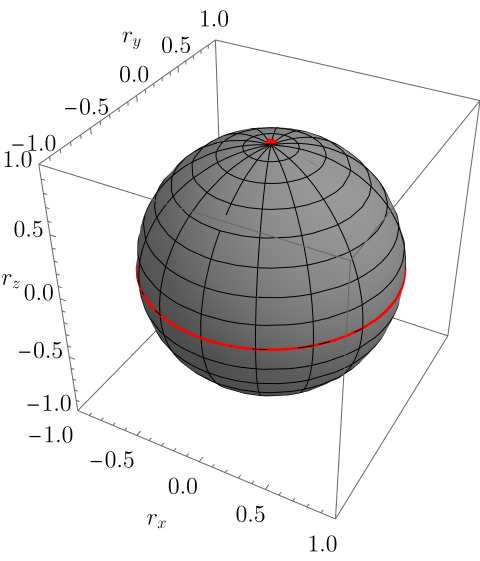
\includegraphics[width=0.9\linewidth]{chapter3/figures_separable/szxId_t=0._p=0.6_r=0.9.png}
      \caption{$t=0.0$}
    \end{subfigure}%
    \begin{subfigure}{0.32\textwidth}
      \centering
      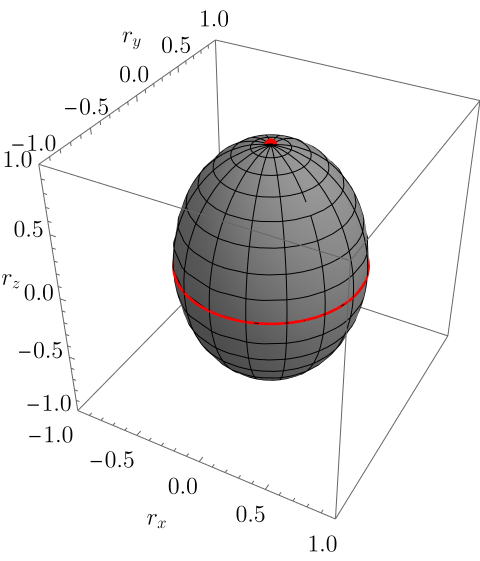
\includegraphics[width=0.9\linewidth]{chapter3/figures_separable/szxId_t=0.25_p=0.6_r=0.9.png}
      \caption{$t=0.25$}
    \end{subfigure}
    \begin{subfigure}{0.32\textwidth}
      \centering
      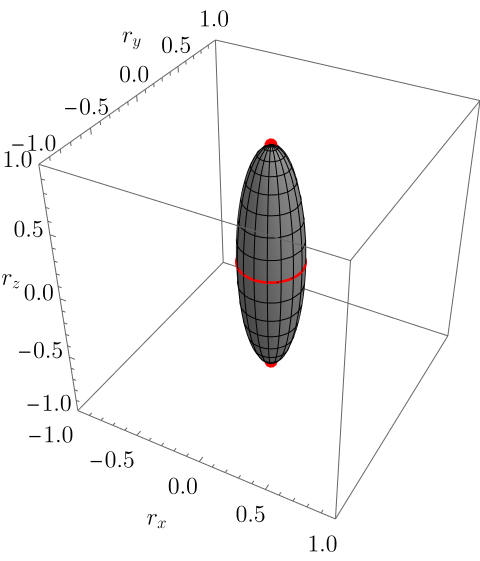
\includegraphics[width=0.9\linewidth]{chapter3/figures_separable/szxId_t=0.5_p=0.6_r=0.9.png}
      \caption{$t=0.5$}
    \end{subfigure}
    \caption{Efecto de la evolución subyacente sobre la esfera de Bloch si $r_{\ef}=0.9$, $p_{1}=0.6$ y $U=e^{-i\pi t \pauli{3}}$. La dramática contracción a lo largo de $z$ se asocia al alto valor de $1-p_{1}$.}
    \label{fig:FaseChangeSequence}
\end{figure}

En efecto, la traslación tiene una magnitud $(1-p_{1})r_{\text{np}}$ (a notar que la traslación es pequeña, y corresponde al término de ruido) en la dirección opuesta a la del estado (i.e. depende del estado tanto en magnitud como en dirección). Así que, aunque esto podría parecer una transformación afín, no lo es, pues depende enteramente del estado. Esto significa que la evolución efectiva no es lineal, y no tiene expresión en términos de operadores de Kraus. La figura \ref{fig:FaseChangeSequence} muestra el efecto que una dinámica de este estilo tiene sobre la esfera de Bloch (en particular, el caso $U_{1}=e^{-\rmi\omega t \pauli{3}}$). La contracción a lo largo del eje $z$ es un resultado del alto valor de $(1-p_{1})$ (0.4), y no sería visible si $p_{1}\rightarrow 1$.


En efecto, si $p_{1}\approx\frac{1}{2}$, entonces $\rho_{1}\approx\rho_{\text{np}}\approx\rho$ y la dinámica efectiva se convertiría en un canal de desfasamiento:

\begin{align}
    \Gamma_{t}(\rho_{\ef})=&p_{1}e^{-\rmi\omega t \pauli{3}}\rho_{1}e^{\rmi\omega t \pauli{3}}+(1-p_{1})\rho_{\text{np}}\nonumber\\
    \approx&\frac{1}{2}(\rho_{\ef}+e^{-\rmi\omega t \pauli{3}}\rho_{\ef} e^{\rmi\omega t \pauli{3}})\nonumber.
\end{align}

\subsubsection{Partícula preferencial invariante}

\acnote{Esta sección la tengo que volver a tocar}

Ahora asumamos que es el sistema preferencial el que no evoluciona, mientras que las demás partículas sí lo hacen. Existen diferentes formas de abordar este problema, según la elección de las probabilidades y de la naturaleza de la evolución del resto de las partículas. Quizá el caso más sencillo es aquel en el que todas las partículas no preferenciales evolucionan de la misma forma. Esto es, una evolución generada por un hamiltoniano de la forma
\begin{equation}
    \mcH=\omega \sum_{k=2}^{n}H_{k}.\nonumber
\end{equation}
Por simplicidad, tómese $H_{k}=\pauli{3}\,\forall k$. Recordando la ecuación (\ref{eq:rhoArhoB}), los valores de expectación de $\pauli{j}$ serán
\begin{align}
    \expval{\pauli{1}(t)}=&p_{1} \expval{\sigma_{1}(0)}_{1}+\sum_{k=2}^{n}p_{k}\Tr[\pauli{1}e^{-\rmi\omega t\pauli{3}} \rho_{k} e^{\rmi\omega t\pauli{3}}]\nonumber\\
    \expval{\pauli{2}(t)}=&p_{1} \expval{\sigma_{2}(0)}_{1}+\sum_{k=2}^{n}p_{k}\Tr[\pauli{2}e^{-\rmi\omega t\pauli{3}} \rho_{k} e^{\rmi\omega t\pauli{3}}]\nonumber\\
    \expval{\pauli{3}(t)}=&\expval{\pauli{3}(0)}_{\ef},\nonumber
\end{align}
que quizá sea más clara escribiéndose en términos de las componentes de los vectores de Bloch de cada partícula (el primer subíndice indica la componente del vector, mientras que el segundo denota la partícula a la que pertenece):
\begin{align}
    r_{1,\ef}(t)=&r_{1,1}(0)+\sum_{k=2}^{n}p_{k}(r_{1,k}\cos(2\omega t)-r_{2,k}\sin(2\omega t))\nonumber\\
    r_{2,\ef}(t)=&r_{2,1}(0)+\sum_{k=2}^{n}p_{k}(r_{2,k}\cos(2\omega t)+r_{1,k}\sin(2\omega t))\nonumber\\
    r_{3,\ef}(t)=&r_{3,\ef}(0).\nonumber
\end{align}
Esto no es más que la aplicación de la misma rotación sobre todos los vectores de Bloch, a excepción del primero. Reescribiendo,
\begin{align}
    \vec{r}_{\ef}(t)=&p_{1}\vec{r}_{1}+R_{z}(2\omega t)\vec{r}_{e}\nonumber\\
    =&\vec{r}_{\ef}(0)+(R_{z}(2\omega t)-\Id)\vec{r}_{e}\nonumber
\end{align}
donde $\vec{r}_{e}\sum_{k=2}^{n}p_{k}\vec{r}_{k}$.
En este caso, el primer término es el término invariante, y sería lo único visible en el caso en que el aparato de medición no fallara, mientras que el segundo término corresponde a pequeñas oscilaciones completamente dependientes del estado efectivo inicial que nunca aumentan la pureza del estado. En efecto, considérese un estado efectivo inicial correspondiente a un sistema microscópico de $10$ qubits cuyo vector de Bloch tiene radio $r_{\ef}=0.95$ y tal que $p_{1}=0.99$ y $p_{j}=\frac{0.01}{9}\,\forall\,j\neq $. La magnitud del error absoluto, esto es, la distancia del estado efectivo evolucionado al estado efectivo inicial es
\begin{equation}
    \mcO_{t}=\norm{\vec{r}_{\ef}(0)-p_{1}\vec{r}_{1}-R_{z}(2\omega t)\vec{r}_{e}}=\norm{\vec{r}_{e}-R_{z}(2\omega t)\vec{r}_{e}}\nonumber.
\end{equation}
Ahora, esta magnitud es máxima cuando $t=\frac{\pi}{2\omega}$, pero depende también de las componentes de $\vec{r}_{ef}$. Por simplicidad, asumamos que el estado efectivo inicial no tiene componente en $z$. Entonces
\begin{equation}
    \mcO_{\max}=\norm{-2\vec{r}_{e}}=1.08\times 10^{-3}\nonumber.
\end{equation}
Estas pequeñas oscilaciones son, justamente, el término de ruido. La visualización a la solución del problema puede observarse en la Figura \ref{fig:OscilationsSameHam}. Cada una de las componentes del vector de Bloch efectivo se ve como una suma de una constante con funciones periódicas que tienen el mismo periodo, o  como la suma de una constante más una función periódica (viendo la combinación de los vectores de cada partícula no preferencial como una partícula efectiva). De cualquier forma, el resultado es una función periódica.

\begin{figure}[ht!]
    \centering
    \begin{subfigure}{0.5\textwidth}
      \centering
      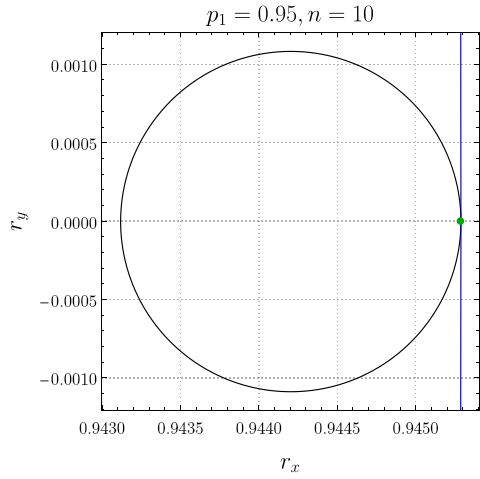
\includegraphics[width=0.9\linewidth]{chapter3/figures_separable/local_prefinv_eq_n=10_p=0.95.png}
      \caption{Nueve no preferencial}
    \end{subfigure}%
    \begin{subfigure}{0.5\textwidth}
      \centering
      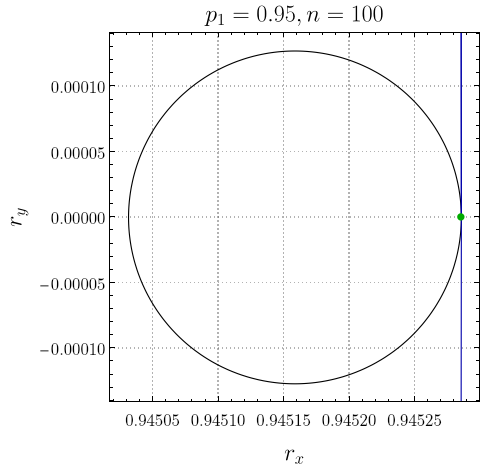
\includegraphics[width=0.9\linewidth]{chapter3/figures_separable/local_prefinv_eq_n=100_p=0.95.png}
      \caption{Noventa y nueve partículas no preferenciales}
    \end{subfigure}
    \caption{Oscilaciones periódicas cercanas al valor esperado. La periodicidad no depende de los pesos probabilísticos de cada partícula. En azul, el conjunto de estados con la misma pureza (y la misma coordenada en $\pauli{3}$) que el estado efectivo inicial (en verde).}\label{fig:OscilationsSameHam}
\end{figure}

Si, por otro lado, quitamos la restricción de que todas las partículas no preferenciales evolucionen con la misma frecuencia, se vuelve imposible factorizar la rotación:
\begin{equation}
    \vec{r}_{\ef}(t)=p_{1}\vec{r}_{1}+\sum_{k=2}^{n} p_{k}R_{z}(2\omega_{k} t)\vec{r}_{k}.\nonumber
\end{equation}
Ahora cada partícula no preferencial contribuye al error de forma única, y a pesar de que la evolución de cada partícula no preferencial sea periódica, la combinación de estas no tiene por qué serlo. El resultado ahora depende de las frecuencias de evolución de cada partícula, de sus pesos $p_{k}$, y del número $n$ de partículas en el sistema microscópico (si $n=2$ se recupera el caso anterior). Las componentes del vector de Bloch del estado efectivo evolucionado,
\begin{align}
    r_{1,\ef}(t)=&r_{1,1}(0)+\sum_{k=2}^{n}p_{k}(r_{1,k}\cos(2\omega_{k} t)-r_{2,k}\sin(2\omega_{k} t))\nonumber\\
    r_{2,\ef}(t)=&r_{2,1}(0)+\sum_{k=2}^{n}p_{k}(r_{2,k}\cos(2\omega_{k} t)+r_{1,k}\sin(2\omega_{k} t))\nonumber\\
    r_{3,\ef}(t)=&r_{3,\ef}(0).\nonumber
\end{align}
revelan la complejidad de la evolución, además de su no-linealidad, pues los vectores $\vec{r}_{k}$ dependen del estado efectivo inicial a través del multiplicador de Lagrange $\lambda.$ Las figuras \ref{fig:PrefInv1} y \ref{fig:PrefInv2} muestran algunos ejemplos de la geometría de estas dinámicas, en las que las frecuencias $\omega_{k}$ se obtuvieron de una distribución uniforme $\text{U}[-3,3]$.

\begin{figure}[ht!]
    \centering
    \begin{subfigure}{0.5\textwidth}
      \centering
      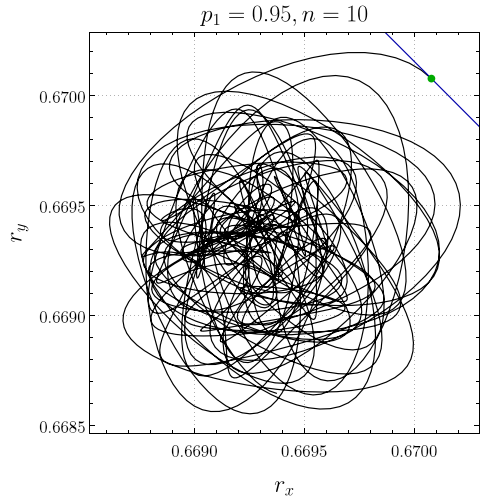
\includegraphics[width=0.9\linewidth]{chapter3/figures_separable/local_prefinv_ran_n=10_p=0.95_r=0.95_a=-3_b=3.png}
    \end{subfigure}%
    \begin{subfigure}{0.5\textwidth}
      \centering
      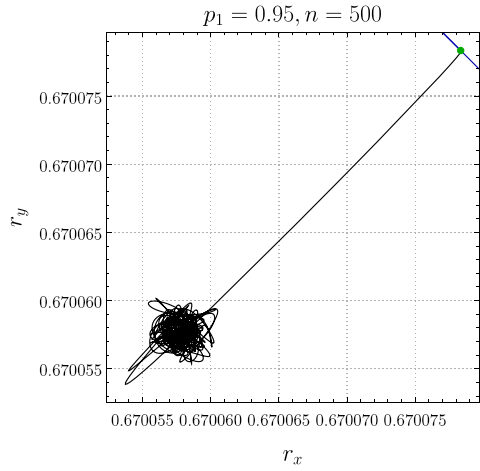
\includegraphics[width=0.9\linewidth]{chapter3/figures_separable/local_prefinv_ran_n=500_p=0.95_r=0.95_a=-3_b=3.png}
    \end{subfigure}
    \caption{Variaciones cercanas al estado efectivo inicial (verde). El aumento en el número de partículas lleva a una evolución complicada y no periódica, pero que converge al punto $\vec{r}_{1}$. En azul, el conjunto de estados con la misma pureza y la misma coordenada en $\pauli{3}$ que el estado efectivo inicial.}\label{fig:PrefInv1}
\end{figure}

\begin{figure}[ht!]
    \centering
    \begin{subfigure}{0.5\textwidth}
      \centering
      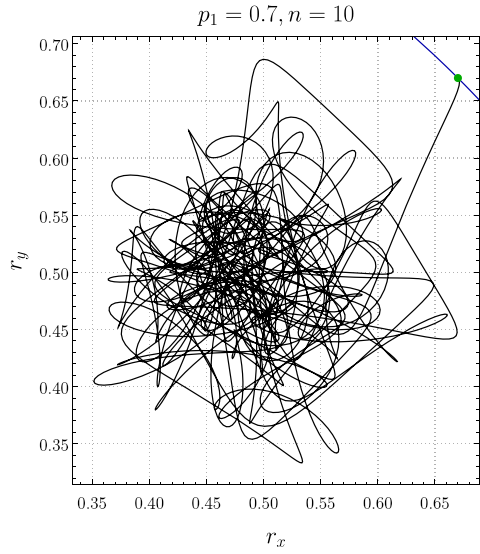
\includegraphics[width=0.9\linewidth]{chapter3/figures_separable/local_prefinv_ran_n=10_p=0.7_r=0.95_a=-3_b=3.png}
    \end{subfigure}%
    \begin{subfigure}{0.5\textwidth}
      \centering
      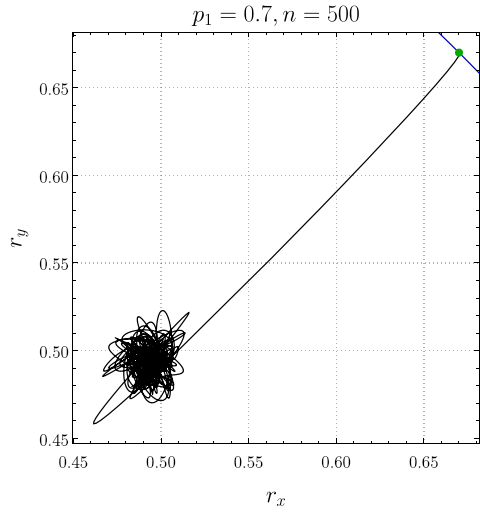
\includegraphics[width=0.9\linewidth]{chapter3/figures_separable/local_prefinv_ran_n=500_p=0.7_r=0.95_a=-3_b=3.png}
    \end{subfigure}
    \caption{Variaciones cercanas al estado efectivo inicial (verde). El aumento en el número de partículas lleva a una evolución complicada y no periódica, pero que converge al punto $\vec{r}_{1}$. Valores menos importantes de $p_{1}$ conducen a mayores variaciones. En azul, el conjunto de estados con la misma pureza y la misma coordenada en $\pauli{3}$ que el estado efectivo inicial.}\label{fig:PrefInv2}
\end{figure}

\subsubsection{Sistema en campo magnético ?}

\acnote{No tengo idea de qué justificación se pueda dar a que todas las partículas oscilen en la misma dirección pero con frecuencias diferentes.}

En los dos casos anteriores se permitió que alguna de las partes del sistema se mantuviera invariante, fuera la partícula preferencial o el resto. Veamos ahora qué sucede cuando se permite que todo el sistema evolucione. Considérese un hamiltoniano
\begin{equation}
    \mcH=\sum_{k=1}^{n}\omega_{k}\pauli{3,k},\nonumber
\end{equation}
de tal forma que toda la evolución mantenga constante la componente en $\pauli{3}$. Explícitamente, las componentes del vector de Bloch del estado efectivo siguen las ecuaciones
\begin{align}
    r_{1,\ef}(t)=&r_{1,1}(t)-\sum_{k=2}^{n}p_{k}A_{k}\sin(2\omega_{k} t-\phi_{k})\nonumber\\
    r_{2,\ef}(t)=&r_{2,1}(t)+\sum_{k=2}^{n}p_{k}A_{k}\sin(2\omega_{k} t+\theta_{k}),\nonumber
\end{align}
donde se omite la tercera componente, que no cambia, y
\begin{align}
    A_{k}=\sqrt{r_{1,k}^{2}+r_{2,k}^{2}} & & \phi=_{k}\arccos\qty(\frac{r_{2,k}}{\sqrt{r_{1,k}^{2}+r_{2,k}^{2}}}) & & \theta_{k}=\arcsin\qty(\frac{r_{1,k}}{\sqrt{r_{1,k}^{2}+r_{2,k}^{2}}})\nonumber
\end{align}
El comportamiento de los términos de suma depende de las frecuencias $\omega_{k}$, pero la amplitud de estas funciones oscilatorias puede acercarse arbitrariamente a $\sum_{k=2}^{n} p_{k} A_{k}$. Esto no significa que el error explote. En realidad, como $0\leq A_{k}\leq 1\,\forall k$, entonces $0\leq\sum_{k=2}^{n} p_{k} A_{k}\leq 1$. 


Para obtener resultados más específicos, asumamos que $p_{j}=p_{\text{np}}=\frac{1-p_{1}}{1-n}\,\forall\,j\neq 1$ y que $r_{3,\ef}=0$. Por construcción del estado de máxima entropía compatible con $\rho_{\ef}$,
\begin{align}
    r_{k}=r_{\text{np}}=\tanh(p_{\text{np}} \lambda) & & r_{j,k}=r_{\text{np}}\frac{r_{j,\ef}}{r_{\ef}}\nonumber
\end{align}
Esto significa que las expresiones previas se simplifican considerablemente, en efecto, las primeras dos componentes del vector pasan a ser
\begin{align}
    r_{1,\ef}(t)&=r_{1,1}(t)-p_{\text{np}}r_{\text{np}}\sum_{k=2}^{n}\sin(2\omega_{k} t-\phi)\nonumber\\
    r_{2,\ef}(t)&=r_{2,1}(t)+p_{\text{np}}r_{\text{np}}\sum_{k=2}^{n}\sin(2\omega_{k} t+\theta)\nonumber
\end{align}
Aquí pasa a ser claro que la amplitud máxima de la oscilación de error de cada componente es $(1-p_{1})r_{\text{np}}$, que en el caso en que $r_{\ef}=0.9$, $p=0.95$ y $n=100$ es $4.79\times 10^{-5}$, pero si $p_{1}=0.5$ es $0.4$. Las figuras \ref{fig:Oscilations12} y \ref{fig:Oscilations13} muestran algunos ejemplos de este tipo de dinámica.

\begin{figure}[ht!]
    \centering
    \begin{subfigure}{0.5\textwidth}
      \centering
      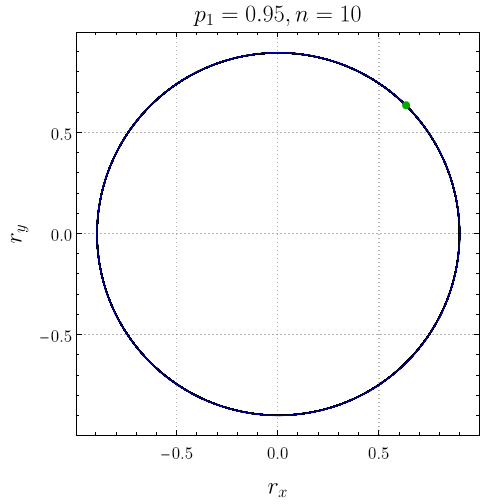
\includegraphics[width=0.9\linewidth]{chapter3/figures_separable/local_all_ran_p=0.95_r=0.9_n=10_a=-3_b=3.png}
    \end{subfigure}%
    \begin{subfigure}{0.5\textwidth}
      \centering
      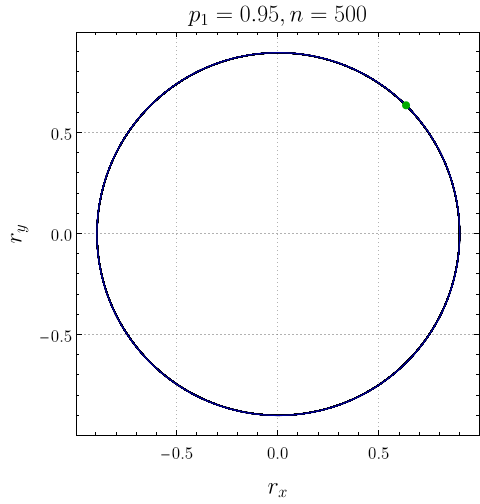
\includegraphics[width=0.9\linewidth]{chapter3/figures_separable/local_all_ran_p=0.95_r=0.9_n=500_a=-3_b=3.png}
    \end{subfigure}
    \caption{Como mencionado, para el caso en que $r_{\ef}=0.9$ y $p=0.95$ las variaciones debidas al error no son perceptibles debido a su pequeña amplitud, independientemente del número de partículas consideradas.}\label{fig:Oscilations12}
\end{figure}
\begin{figure}[ht!]
    \centering
    \begin{subfigure}{0.5\textwidth}
      \centering
      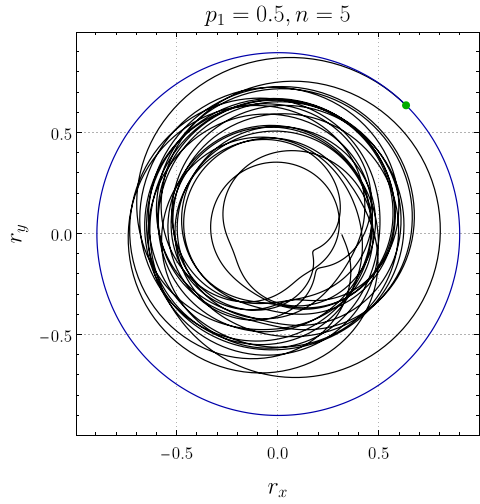
\includegraphics[width=0.9\linewidth]{chapter3/figures_separable/local_all_ran_p=0.5_r=0.9_n=5_a=-3_b=3.png}
    \end{subfigure}%
    \begin{subfigure}{0.5\textwidth}
      \centering
      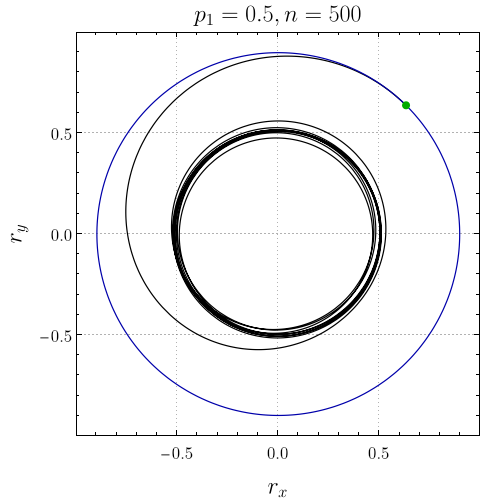
\includegraphics[width=0.9\linewidth]{chapter3/figures_separable/local_all_ran_p=0.5_r=0.9_n=500_a=-3_b=3.png}
    \end{subfigure}
    \caption{Si $r_{\ef}=0.9$ y $p=0.3$, el alejamiento de la evolución esperada se hace notar. Para valores grandes de $n$ se vuelve dominante el término de $p_{1}$}\label{fig:Oscilations13}
\end{figure}

\newpage

\pagebreak
\section{Construcción de la dinámica}
\notaAd{USAR MAPSTO EN LUGAR DE XRIGHTARROW}
\subsection{La compuerta cuántica SWAP}

\subsubsection{Acción de la compuerta}
La compuerta SWAP, $S$, actúa sobre dos qubits y los \textit{voltea}. Su acción sobre la base de $\hilbert_{4}$ contruida mediante los eigenestados de $\sigma_{3}\otimes\sigma_{3}$ es
\begin{align*}
    \ket{0}\otimes\ket{0}\xrightarrow{S}\ket{0}\otimes\ket{0}\\
    \ket{0}\otimes\ket{1}\xrightarrow{S}\ket{1}\otimes\ket{0}\\
    \ket{1}\otimes\ket{0}\xrightarrow{S}\ket{0}\otimes\ket{1}\\
    \ket{1}\otimes\ket{1}\xrightarrow{S}\ket{1}\otimes\ket{0} \rlap{.}
\end{align*}
Si un sistema está descrito por un operador de densidad separable, $\varrho=\rho_{A}\otimes\rho_{B}$, entonces el efecto de la compuerta SWAP es 
\begin{equation*}
    S\varrho S^{\dag}=\rho_{B}\otimes\rho_{A}.
\end{equation*}
La compuerta puede representarse como una matriz de permutación
\begin{equation*}
    S=\begin{pmatrix}
        1&0&0&0\\
        0&0&1&0\\
        0&1&0&0\\
        0&0&0&1
    \end{pmatrix}
\end{equation*}
\subsubsection{SWAP completo efectivo}

Utilizando la expresión (\ref{eq:MaxEntSeparable}), se puede pasar tanto a $\varrho_{max}(0)$ como a $\varrho_{max}(1)$ a través de la aplicación de grano grueso. El resultado $\CG{\varrho_{max}(0)}$ corresponde al estado grueso inicial, pero en términos de $\lambda$. Así:
\begin{equation}
\rho(0)=\frac{1}{2}[\Id+(\hat{r}_{\rho}\cdot\vec{\sigma})(p\tanh{-\lambda p}+(1-p)\tanh{-\lambda (1-p)})],
\end{equation}
\begin{equation}
\rho(t=1)=\frac{1}{2}[\Id+(\hat{r}_{\rho}\cdot\vec{\sigma})((1-p)\tanh{-\lambda p}+p\tanh{-\lambda (1-p)})].
\end{equation}
Vemos que ambos estados tienen la misma orientación pero pureza distinta. Esto significa que el efecto del \textsc{SWAP} subyacente sobre la esfera de Bloch es comprimir al estado efectivo inicial con un coeficiente $\kappa_{1}$ tal que
\begin{equation}\label{eq:SWAPFactor}
  \kappa_{1}=\frac{r_{\rho(1)}}{r_{\rho(0)}}=\frac{(1-p)\tanh{\lambda p}+p\tanh{\lambda (1-p)}}{
    p\tanh{\lambda p}+(1-p)\tanh{\lambda (1-p)}}
\end{equation}
Claro está, el factor de compresión depende del multiplicador de Lagrange, que a su vez es una función de la pureza del estado inicial. La figura \ref{fig:SWAPFactor2D} muestra dicha dependencia. Si la dependencia del factor de compresión en el estado efectivo inicial se denota por un superíndice, la dinámica efectiva puede escribirse como
\begin{equation}\label{eq:EffectiveSWAP1}
  \boxed{\frac{1}{2}(\Id+\vec{r}_{\rho}\cdot\vec{\sigma}) \xrightarrow{S} \frac{1}{2}(\Id+\kappa_{1}^{\rho}\vec{r}_{\rho}\cdot\vec{\sigma})}
\end{equation}
De las ecuaciónes (\ref{eq:SWAPFactor}) y (\ref{eq:EffectiveSWAP1}) distinguimos lo siguiente:
\begin{itemize}
  \item Si $p=0.5$, entonces $\kappa_{1}^{\rho}=1$. Esto se debe a que la aplicación borrosa es invariante bajo el $\textsc{SWAP}$ si $p=0.5$.
  \item $\kappa_{1}^{\rho}$ no depende de la orientación del vector de Bloch, únicamente depende de la magnitud $r_{\rho(0)}$ y $p$.
  \item En los casos extremos, $p=1$ o $p=0$, la esfera colapsa al origen.
\end{itemize}


Como el factor de compresión depende de $\lambda$, la dinámica no es lineal. Las operaciones cuánticas de un qubit se traducen como aplicaciones afines en la esfera de Bloch. Si quisiéramos ver el proceso asociado al \textsc{SWAP} subyacente como una transformación de la forma
\begin{equation*}
  \vec{r}\rightarrow M\vec{r}+\vec{c}
\end{equation*}
en la que $\vec{c}=0$, y $M=OS$ con $O=\Id$ y $S=\kappa_{1}(\vec{r})\Id$, de tal forma que
\begin{equation*}
  \vec{r}\rightarrow \kappa_{1}(\vec{r})\vec{r}
\end{equation*}
nos daríamos cuenta que la transformación no es afín, y por esto, el proceso no puede ser descrito a través del formalismo de las operaciones cuánticas (no tiene representación en operadores de Kraus) \cite{Chuang}.
\subsubsection{Caso $p=\frac{1}{2}$}

Aunque es posible repetir todas las cuentas desde la contrucción del estado de máxima entropía, haciendo $p=\frac{1}{2}$, basta con ver que el factor (\eqref{eq:SWAPFactor}) es $1$ en dicho caso. Así, todos los estado gruesos son puntos fijos bajo una evolución subyacente SWAP con aplicación de grano grueso con parámetro $p=\frac{1}{2}$.

\subsubsection{SWAP efectivo a un tiempo arbitrario}
Siendo \textsc{SWAP} un operador unitario, anteriormente se denotó el estado inicial y final como $\varrho(0)$ y $\varrho(1)$, de acuerdo a lo establecido en la ecuación (\ref{eq:TimeDepenenceUnitary}). Para extender los resultados a un tiempo arbitrario en el intervalo $[0,1]$, es necesaria una expresión analítica del operador. El operador SWAP deja intactos a los estados $\ket{00}$ y $\ket{11}$, e intercambia $\ket{01}$ con $\ket{1,0}$. De esto, el operador también dejará invariantes (hasta un factor) a los estados $\ket{+_{2}}=\frac{\ket{01}+\ket{10}}{\sqrt{2}}$ y $\ket{-_{2}}\frac{\ket{01}-\ket{10}}{\sqrt{2}}$. Dados estos eigenestados (y eigenvalores), la descomposición espectral del operador es
\begin{equation}\label{eq:SWAPSpectral}
S=P(\dyad{00}+\dyad{11}+\dyad{+_{2}}-\dyad{-_{2}})P^{\dag}.
\end{equation}
donde $P$ es la matriz formada por los eigenestados del operador. Potenciando se halla que
\begin{align}\label{eq:SWAPPower}
S^{t}&=P(\dyad{00}+\dyad{11}+\dyad{+_{2}}+(-)^{t}\dyad{-_{2}})P^{\dag}\\
&=P(\dyad{00}+\dyad{11}+\dyad{+_{2}}+e^{i \pi t}\dyad{-_{2}})P^{\dag}
\end{align}
La forma matricial del operador \textsc{SWAP} a un tiempo $t$ es
\begin{equation}
S^{t}=\begin{pmatrix}
 1 & 0 & 0 & 0 \\
 0 & \frac{1}{2}(1+e^{i \pi t}) & \frac{1}{2} (1-e^{i \pi t}) & 0 \\
 0 & \frac{1}{2}(1-e^{i \pi t}) & \frac{1}{2}(1+e^{i \pi t}) & 0 \\
 0 & 0 & 0 & 1
\end{pmatrix}=\begin{pmatrix}
  1 & 0 & 0 & 0 \\
  0 & e^{i\frac{t\pi}{2}}\cos{\frac{t\pi}{2}} & -ie^{i\frac{t\pi}{2}}\sin{\frac{t\pi}{2}} & 0 \\
  0 & -ie^{i\frac{t\pi}{2}}\sin{\frac{t\pi}{2}} & e^{i\frac{t\pi}{2}}\cos{\frac{t\pi}{2}}  & 0 \\
  0 & 0 & 0 & 1
 \end{pmatrix}
\end{equation}
Con ayuda de Mathematica pude aplicar este operador para obtener que
\begin{equation}
  \rho(t)=\frac{1}{2}\{\Id-(\hat{r_{\rho}}\cdot\vec{\sigma})[((1-p)\cos^{2}{\frac{\pi t}{2}}+p\sin^{2}{\frac{\pi t}{2}})\tanh{p\lambda}+(p\cos^{2}{\frac{\pi t}{2}}+(1-p)\sin^{2}{\frac{\pi t}{2}})\tanh{(1-p)\lambda}]\}.
\end{equation}
De esto, el factor de compresión dependiente del tiempo es
\begin{equation}\label{eq:SWAPFactort}
  \kappa_{t}^{\rho}=\frac{((1-p)\cos^{2}{\frac{\pi t}{2}}+p\sin^{2}{\frac{\pi t}{2}})\tanh{\lambda p}+(p\cos^{2}{\frac{\pi t}{2}}+(1-p)\sin^{2}{\frac{\pi t}{2}})\tanh{\lambda (1-p)}}{
    p\tanh{\lambda p}+(1-p)\tanh{\lambda (1-p)}}
\end{equation}
En términos del valor esperado del observable $\sigma_{z}$, la evolución del estado se da como
\begin{equation}
  \expval{\sigma_{z}(t)}=\kappa_{t}^{\rho}\cos{\alpha}
\end{equation}
que puede escribirse, también, como las probabilidades de que $\rho(t)$ se halle en el estado $\ket{0}$ o $\ket{1}$
 \begin{align}
  \bra{0}\rho(t)\ket{0}=\frac{1}{2}(1+\kappa_{t}^{\rho}\cos{\alpha}) && \bra{1}\rho(t)\ket{1}=\frac{1}{2}(1-\kappa_{t}^{\rho}\cos{\alpha})
 \end{align}
 donde la dependencia temporal está completamente contenida dentro del factor $\kappa_{t}^{\rho}$. 

\subsection{La compuerta cuántica CNOT}

\subsubsection{Acción de la compuerta}

La compuerta \textit{controlled not}, o CNOT, es el análogo cuántico de la compuerta lógica XOR \notaAd{CITA}. La compuerta XOR recibe como entrada dos bits, y arroja uno que puede ser $0$ si los bits de entrada tienen el mismo valor, o $1$ si tienen valores diferentes. Por otro lado, la compuerta cuántica CNOT actúa sobre un sistema de dos qubits, aplicando sobre el segundo qubit la compuerta $\sigma_{1}$ (NOT) si el primer qubit se halla en el estado $\ket{1}$, o dejándolo invariante si el primer qubit se halla en el estado $\ket{0}$. Esto es, cumple que \notaAd{CITA}
\begin{align*}
    \ket{0}\otimes\ket{0}\xrightarrow{\cnot}\ket{0}\otimes\ket{0}\\
    \ket{0}\otimes\ket{1}\xrightarrow{\cnot}\ket{0}\otimes\ket{1}\\
    \ket{1}\otimes\ket{0}\xrightarrow{\cnot}\ket{1}\otimes\ket{1}\\
    \ket{1}\otimes\ket{1}\xrightarrow{\cnot}\ket{1}\otimes\ket{0} \rlap{.}
\end{align*}
La compuerta puede representarse como una matriz de permutación
\begin{equation*}
    \cnot=\begin{pmatrix}
        1&0&0&0\\
        0&1&0&0\\
        0&0&0&1\\
        0&0&1&0
    \end{pmatrix}
\end{equation*}

\section{Dinámicas especiales}

\subsection{Canales de Pauli}

Los canales de Pauli son canales cuánticos en los que se aplica un operador de Pauli con alguna probabilidad. El canal de Pauli de un qubit más general está definido como
\begin{gather}
    P:\mcB(\hilbert_{2}) \rightarrow \mcB(\hilbert_{2})\nonumber\\
    P(\Delta)=\sum_{j=0}^{3}q_{j}\pauli{j}\Delta\pauli{j}\,\text{ con }\, \sum_{j=0}^{3}q_{j}=1\rlap{.}\nonumber
\end{gather}
Reconociendo que cualquiera de los tres operadores de Pauli puede escribirse en términos de los otros dos, se puede aprovechar la relación $-i\pauli{2}=\pauli{1}\pauli{3}$ para escribir a los canales de Pauli de una forma particularmente útil:
\begin{equation}
    P(\Delta)=\sum_{j,k=0}^{1}q_{j,k}\pauli{1}^{j}\pauli{3}^{k}\Delta\pauli{3}^{k}\pauli{1}^{j}.\nonumber
\end{equation}
A través de esta expresión se extienden los canales de Pauli de un qubit a $n$ qubits como \acnote{agregar cita}
\begin{gather}\label{eq:PauliChannelN}
    P:\mcB(\hilbert_{2^{n}}) \rightarrow \mcB(\hilbert_{2^{n}})\nonumber\\
    P(\Delta)=\sum_{\vec{j},\vec{k}}q_{\vec{j},\vec{k}}\pauli{1}^{\vec{j}}\pauli{3}^{\vec{k}}\Delta\pauli{3}^{\vec{k}}\pauli{1}^{\vec{j}}\rlap{.}
\end{gather}
donde $\pauli{j}^{\vec{k}}=\pauli{j}^{k_{1}}\otimes\pauli{j}^{k_{2}}\otimes ... \otimes \pauli{j}^{k_{n}}$ y las entradas $k_{l}$ del vector $\vec{k}$ solo pueden valer $0$ o $1$.

\subsubsection{Canales de desfasamiento}

Por canales de desfasamiento se entiende aquellos canales cuánticos cuyo efecto es amortiguar los elementos fuera de la diagonal del operador sobre el que actúan. A notar que esta definición es dependiente de la base sobre la que se está trabajando. Por ejemplo, sea $\rho\in\densityspace{2}$. Si se utiliza la base de eigenestados de $\pauli{3}$, entonces el canal
\begin{equation}
    \rho\mapsto q_{1}\rho + q_{2} \pauli{3}\rho\pauli{3}\nonumber
\end{equation}
es un canal de desfasamiento. En efecto, la acción de este canal sobre los elementos de matriz de $\rho$ es
\begin{equation}
    \begin{pmatrix}
        \rho_{0,0} & \rho_{0,1}\\
        \rho_{1,0} & \rho_{1,1}\\
    \end{pmatrix}\mapsto\begin{pmatrix}
        \rho_{0,0} & (q_{1}-q_{2})\rho_{0,1}\\
        (q_{1}-q_{2})\rho_{1,0} & \rho_{1,1}\\
    \end{pmatrix},\nonumber
\end{equation}
mientras que el canal de \textit{bit flip},
\begin{equation}
    \rho\mapsto q_{1}\rho + q_{2} \pauli{1}\rho\pauli{1},\nonumber
\end{equation}
no lo es, pues su acción sobre los elementos de matriz de $\rho$ es
\begin{equation}
    \begin{pmatrix}
        \rho_{0,0} & \rho_{0,1}\\
        \rho_{1,0} & \rho_{1,1}\\
    \end{pmatrix}\mapsto\begin{pmatrix}
        \frac{1}{2}\qty(1+(q_{1}-q_{2})(2\rho_{0,0}-1)) & \Re(\rho_{0,1})-\rmi(q_{1}-q_{2})\Im(\rho_{0,1})\\
        \Re(\rho_{1,0})+\rmi(q_{1}-q_{2})\Im(\rho_{1,0}) & \frac{1}{2}\qty(1-(q_{1}-q_{2})(1-2\rho_{1,1}))\\
    \end{pmatrix}.\nonumber
\end{equation}
Por supuesto, el canal de \textit{bit flip} es un canal de desfasamiento si se trabaja en la base de los eigenestados de $\pauli{1}$, pues en esta base, la acción del canal de \textit{bit flip} es
\begin{equation}
    \begin{pmatrix}
        \rho_{0,0} & \rho_{0,1}\\
        \rho_{1,0} & \rho_{1,1}\\
    \end{pmatrix}\mapsto\begin{pmatrix}
        \rho_{0,0} & (q_{1}-q_{2})\rho_{0,1}\\
        (q_{1}-q_{2})\rho_{1,0} & \rho_{1,1}\\
    \end{pmatrix}.\nonumber
\end{equation}
Para extender la noción de canal de desfasamiento a $n$ qubits, primero nótese que dada la base de $\hilbert_{2}$ conformada por los eigenestados de $\sigma{3}$, $\{\ket{e_{0}},\ket{e_{1}}\}$, es posible construir una base $\{e_{\vec{k}}\}_{\vec{k}}$ de $\hilbert_{2^{n}}$ como
\begin{equation}
    \{e_{\vec{k}}\}_{\vec{k}}=\left\{\ket{e_{\vec{k}}}\in\hilbert_{2^{n}}: \ket{e_{\vec{k}}}=\Motimes_{j=1}^{n}\ket{e_{k_{j}}},\,k_{j}\in\{0,1\}\right\} \rlap{.}\nonumber
\end{equation}
Esto es, tomando los productos tensoriales de los eigenestados de $\pauli{3}$ consigo mismos. De esta manera podemos estudiar dos canales de desfasamiento, el primero actuando en la base de productos tensoriales de eigenestados de $\pauli{3}$,
\begin{gather}
    P_{\pauli{3}}:\mcB(\hilbert_{2^{n}}) \rightarrow \mcB(\hilbert_{2^{n}})\nonumber\\
    P_{\pauli{3}}(\Delta)=\sum_{\vec{k}}q_{\vec{k}}\pauli{3}^{\vec{k}}\Delta\pauli{3}^{\vec{k}}\rlap{,}\nonumber
\end{gather}
que corresponde al canal de Pauli \ref{eq:PauliChannelN} cuando $\vec{j}=0$, y el segundo definido sobre la base de productos tensoriales de eigenestados de $\pauli{1}$,
\begin{gather}
    P_{\pauli{1}}:\mcB(\hilbert_{2^{n}}) \rightarrow \mcB(\hilbert_{2^{n}})\nonumber\\
    P_{\pauli{1}}(\Delta)=\sum_{\vec{j}}q_{\vec{j}}\pauli{1}^{\vec{j}}\Delta\pauli{1}^{\vec{j}}\rlap{,}\nonumber
\end{gather}
que corresponde al canal de Pauli \ref{eq:PauliChannelN} cuando $\vec{k}=0$. Es relativamente sencillo demostrar que si se escoge $q_{\vec{j}}=\frac{1-q_{\vec{0}}}{2^{n}-1}\,\forall\,\vec{j}\neq\vec{0}$, el efecto de estos canales es de reducir la amplitud de las componentes fuera de la diagonal en un factor de $(2q_{\vec{0}}-1)$. \acnote{Debe ser sencillo, el problema es que me hago bolas con los índices.}

Consideremos entonces en canal de desfasamiento de dos qubits en cualquiera de las dos direcciones discutidas y con probabilidades como mencionadas anteriormente. Sea $\rho_{\ef}$ un estado efectivo en $\densityspace{2}$ correspondiente a un sistema $\varrho \in \densityspace{2^{n}}$, y sea $\varrho_{\max}\in\densityspace{2^{n}}$ el estado de máxima entropía compatible con el estado efectivo. Si se propaga al estado de máxima entropía por medio de este canal y luego se pasa el resultado por la aplicación de grano grueso, el resultado es una dinámica efectiva
\begin{equation}
  \Gamma_{t}(\rho_{\ef})=\mcC\qty[\sum_{\vec{j}}q_{\vec{j}}\,\pauli{3}^{\vec{j}}\varrho_{\max}\pauli{3}^{\vec{j}}]=\mcC\qty[\sum_{\vec{j}}q_{\vec{j}}\,\qty(\Motimes_{k=1}^{n} \pauli{3}^{j_{k}}\rho_{k}\pauli{3}^{j_{k}})]\nonumber.\nonumber
\end{equation}
Para resolver el lado derecho de la ecuación, nótese que existen $2^{n}$ posibles vectores $\vec{j}$, y dentro de estos, $2^{n-1}$ tienen un $0$ o un $1$ en la $\nu$-ésima posición. Esto significa que hay $\frac{2^{n-1}}{n}$ ceros y $\frac{2^{n-1}}{n}$ unos en cada posible entrada de todos los $\vec{j}$. Entonces podemos usar el hecho de que tanto los operadores $\pauli{3}^{\vec{j}}$ como el estado de máxima entropía son factorizables, así como que la aplicación de grano es lineal para sumar sobre dichos ceros y unos:
\begin{align}
    \mcC\qty[\sum_{\vec{j}}q_{\vec{j}}\,\qty(\Motimes_{k=1}^{n} \pauli{3}^{j_{k}}\rho_{k}\pauli{3}^{j_{k}})]=&\sum_{\vec{j}}q_{\vec{j}}\sum_{k=1}^{n}p_{k}\pauli{3}^{j_{k}}\rho_{k}\pauli{3}^{j_{k}}\nonumber\\
    =&\sum_{\{j_{k}:j_{k}=0\}}q_{j_{k}}\sum_{k=1}^{n}p_{k}\pauli{3}^{j_{k}}\rho_{k}\pauli{3}^{j_{k}}+\sum_{\{j_{k}:j_{k}=1\}}q_{j_{k}}\sum_{k=1}^{n}p_{k}\pauli{3}^{j_{k}}\rho_{k}\pauli{3}^{j_{k}}\nonumber\\
    =&q_{\vec{0}}\qty(\sum_{k=1}^{n}p_{k}\rho_{k})+\frac{1-q_{\vec{0}}}{2^{n}-1}(2^{n-1}-1)\qty(\sum_{k=1}^{n}p_{k}\rho_{k})+\frac{1-q_{\vec{0}}}{2^{n}-1}2^{n-1}\qty(\sum_{k=1}^{n}\pauli{3}p_{k}\rho_{k}\pauli{3}).\nonumber
\end{align}
Con lo que la dinámica efectiva es
\begin{equation}
    \Gamma_{t}(\rho_{\ef})=\qty(q_{\vec{0}}+\frac{2^{n-1}-1}{2^{n}-1}(1-q_{\vec{0}}))\rho_{\ef}+\qty(\frac{2^{n-1}}{2^{n}-1}(1-q_{\vec{0}}))\pauli{3}\rho_{\ef}\pauli{3}.\nonumber
\end{equation}
Nótese que la dinámica efectiva es lineal, y que únicamente depende de del número de partículas en el sistema microscópico. Aún más, este es un canal de desfasamiento de un qubit en dirección de $\pauli{3}$. Este resultado es análogo para el canal $P_{\pauli{1}}$. Para recuperar un canal de desfasamiento total (en el que todos los elementos fuera de la diagonal se hacen cero) basta con elegir $q_{\vec{j}}=\frac{1}{2^{n}}\,\forall\,\vec{j}$. En dicho caso la dinámica efectiva se reduce a
\begin{equation}
    \Gamma_{t}(\rho_{\ef})=\frac{1}{2}(\rho_{\ef}+\pauli{3}\rho_{\ef}\pauli{3}).\nonumber
\end{equation}
Esto es, el desfasamiento total en $n$ partículas se traduce como un desfasamiento total en una partícula.


\subsubsection{Canal de despolarización}

El canal de despolarización es el canal cuántico que contrae de manera uniforme a todos los estados hacia el estado máximamente mezclado. Al canal de despolarización se le define como
\begin{gather}\label{eq:DepolarizingChannelN}
    D_{q}:\mcB(\hilbert_{2^{n}}) \rightarrow \mcB(\hilbert_{2^{n}})\nonumber\\
    D_{q}(\Delta)=q\Delta+(1-q)\Id_{2^{n}}\Tr(\Delta)\rlap{.}
\end{gather}
Ahora, nótese que el canal de despolarización total puede verse como una concatenación de dos canales de desfasamiento total, uno en dirección $\pauli{1}$ y luego otro en dirección $\pauli{3}$ (el orden es irrelevante). Para ver esto, es particularmente útil escribir a la matriz de densidad $\varrho\in\densityspace{2^{n}}$ en términos de las componentes de su vector de Bloch,
\begin{equation}
    \varrho=\frac{1}{2^{n}}\sum_{\vec{j},\vec{k}}\gamma_{\vec{j},\vec{k}}\pauli{1}^{\vec{j}}\pauli{3}^{\vec{k}},\nonumber
\end{equation}
y notar que el efecto de dichos canales se puede ver como
\begin{align}
  P_{\pauli{1}}(\varrho)=\frac{1}{2^{n}}\sum_{\vec{j},\vec{k}}\delta_{\vec{k},\vec{0}}\gamma_{\vec{j},\vec{k}}\pauli{1}^{\vec{j}}\pauli{3}^{\vec{k}}  & & \text{y} & & P_{\pauli{3}}(\varrho)=\frac{1}{2^{n}}\sum_{\vec{j},\vec{k}}\delta_{\vec{j},\vec{0}}\gamma_{\vec{j},\vec{k}}\pauli{1}^{\vec{j}}\pauli{3}^{\vec{k}} \nonumber
\end{align}
de tal forma que su composición es
\begin{align}
    \qty(P_{\pauli{1}}\circ P_{\pauli{3}})(\varrho)&=\frac{1}{2^{n}}\sum_{\vec{j},\vec{k}}\delta_{\vec{j},\vec{0}}\delta_{\vec{k},\vec{0}}\gamma_{\vec{j},\vec{k}}\pauli{1}^{\vec{j}}\pauli{3}^{\vec{k}}\nonumber\\
    &=\frac{1}{2^{n}}\gamma_{\vec{0},\vec{0}}\Id_{2^{n}}.\nonumber
\end{align}
Que es precisamente el efecto del canal de despolarización total. Ahora, sea $\rho_{\ef}$ un estado efectivo en $\densityspace{2}$ correspondiente a un sistema $\varrho \in \densityspace{2^{n}}$, y sea $\varrho_{\max}\in\densityspace{2^{n}}$ el estado de máxima entropía compatible con el estado efectivo. Es inmediato ver que la dinámica efectiva correspondiente a un canal de despolarización total es otro canal de despolarización total, i.e.
\begin{equation}
    \Gamma_{t}(\rho_{\ef})=\frac{1}{2}\Id_{2}.
\end{equation}
Ahora, sabiendo que
\begin{equation}
    \qty(P_{\pauli{1}}\circ P_{\pauli{3}})(\varrho)=\frac{1}{2^{2n}}\sum_{\vec{j},\vec{k}}\pauli{1}^{\vec{j}}\pauli{3}^{\vec{k}}\varrho\pauli{3}^{\vec{k}}\pauli{1}^{\vec{j}}=\frac{1}{2^{n}}\Id_{2^{n}}\nonumber
\end{equation}
la ecuación \ref{eq:DepolarizingChannelN} puede reescribirse como
\begin{equation}
    D_{q}(\varrho)=\frac{q(2^{2n}-1)+1}{2^{2n}}\varrho+\frac{(1-q)}{2^{2n}}\sum_{\vec{j}\land\vec{k}\neq\vec{0}}\pauli{1}^{\vec{j}}\pauli{3}^{\vec{k}}\varrho\pauli{3}^{\vec{k}}\pauli{1}^{\vec{j}}\nonumber
\end{equation}
Donde es explícitamente claro que el canal de despolarización es un canal de Pauli. La dinámica efectiva que corresponde al canal de despolarización no completo es simplemente
\begin{equation}
    \Gamma_{t}(\rho_{\ef})=q\rho_{\ef}+(1-q)\Id_{2}.\nonumber
\end{equation}
Esto es, la dinámica efectiva correspondiente a un canal de despolarización siempre es un canal de despolarización. Nótese que este resultado es muy similar al obtenido para una evolución unitaria subyacente generada por un Hamiltoniano de la forma $\mcH=H\otimes\Id+\Id\otimes H$. En dicho caso, la dinámica efectiva era, justamente, la unitaria generada por el Hamiltoniano $H$, esto como consecuencia de la simetría de la evolución: la misma para cada partícula, sin interacción. Este caso es el mismo, el canal de despolarización actúa de la misma forma sobre cada partícula, y es completamente isotrópico dentro del subespacio de cada partícula.

\subsection{Canal de estabilización}

El canal de amortiguamiento de amplitud funciona como un modelo simple de emisión espontánea. En efecto, un átomo de dos niveles acoplado a un campo electromagnético experimenta emisión espontánea, y puede demostrarse que este proceso corresponde a un canal de amortiguamiento de amplitud si se traza al campo y se considera que la frecuencia del campo es igual a la frecuencia de resonancia de transiciones entre los niveles del átomo. El canal de amortiguamiento de amplitud tiene el efecto de enviar todos los estados al estado base. Aquí estudiaremos un canal más sencillo, que envía todos los estados a un estado puro aleatorio $\ket{\psi}$ de forma exponencial en el tiempo, como si el átomo de dos niveles tendiera a estabilizarse en dicho estado.

Considérese entonces que un sistema de $n$ partículas evoluciona siguiendo el canal cuántico
\begin{gather}
    \mcE_{\psi,t}:\mcB(\hilbert_{2^{n}}) \rightarrow \mcB(\hilbert_{2^{n}})\nonumber\\
    \mcE_{\psi,t}(\Delta)=e^{-t\mu}\varrho+(1-e^{-t \mu})\dyad{\psi}\Tr(\Delta)\rlap{.}\nonumber
\end{gather}
donde $\dyad{\psi}\in \densityspace{2^{n}}$. Es importante señalar que si se escoge $n=1$ y $\ket{\psi}=\ket{0}$ no se recupera el canal de amortiguamiento de amplitud, pues el canal de amortiguamiento de amplitud tiene el siguiente efecto sobre la matriz de densidad
\begin{equation}
    \begin{pmatrix}
        \rho_{0,0} & \rho_{0,1} \\
        \rho_{1,0} & \rho_{1,1}
    \end{pmatrix}\mapsto\begin{pmatrix}
        (1-\gamma)\rho_{0,0}+\gamma & \sqrt{1-\gamma}\rho_{0,1} \\
        \sqrt{1-\gamma}\rho_{1,0} & (1-\gamma)\rho_{1,1}
    \end{pmatrix},\nonumber
\end{equation}
donde $\gamma$ puede verse como la probabilidad de emisión de un fotón, mientras que el canal $\mcE_{\ket{0},t}$ tiene el efecto
\begin{equation}
    \begin{pmatrix}
        \rho_{0,0} & \rho_{0,1} \\
        \rho_{1,0} & \rho_{1,1}
    \end{pmatrix}\mapsto\begin{pmatrix}
        (1-\gamma)\rho_{0,0}+\gamma & (1-\gamma)\rho_{0,1} \\
        (1-\gamma)\rho_{1,0} & (1-\gamma)\rho_{1,1}
    \end{pmatrix}.\nonumber
\end{equation}
donde se ha hecho $e^{\mu t}=\gamma$. Es claro que el canal de amortiguamiento y el canal de estabilización tienen efectos diferentes en las fases del estado. Aún más, mientras que la extensión del canal de estabilización a $n$ partículas es directa, la generalización del canal de amortiguamiento de amplitud es no trivial. \acnote{agregar cita.}

Ahora, sea $\rho_{\ef}$ un estado efectivo en $\densityspace{2}$ y $\varrho_{\max}$ el estado de máxima entropía en $\densityspace{2^{n}}$ compatible con este. Aplicando el modelo de grano grueso al estado de máxima entropía propagado por el canal de estabilización se obtiene que
\begin{equation}
    \Gamma_{t}(\rho_{\ef})=e^{-t\mu}\rho(0)+(1-e^{-t \mu})\mcC(\dyad{\psi}).\nonumber
\end{equation}
Obsérvese que la dinámica efectiva es un canal cuántico, pero no necesariamente un canal de estabilización, pues el estado al que tiende el sistema efectivo, $\mcC(\dyad{\psi})$ no tiene por qué ser un estado puro. En realidad, en el caso en que $\ket{\psi}$ es un estado máximamente entrelazado, $\mcC(\dyad{\psi})$ es el estado máximamente mezclado, de tal manera que la dinámica efectiva es un canal de despolarización.

\subsection{Cadena de espines de Heisenberg}

El modelo $XZY_{s}$ unodimensional de Heisenberg consiste en una cadena de $n$ partículas de espín $s$ en la que se consideran interacciones de espín entre primeros vecinos. Se ha demostrado que la cadena de Heisenberg describe el comportamiento de algunos metales y cristales \acnote{cita}. El hamiltoniano del modelo de Heisenberg en el caso de espín $\frac{1}{2}$ es
\begin{equation}
    H=\sum_{k=1}^{n}\qty(J_{1}\pauli{1,k}\pauli{1,k+1}+J_{2}\pauli{2,k}\pauli{2,k+1}+J_{3}\pauli{3,k}\pauli{3,k+1})-g\sum_{k=1}^{n}\pauli{2,k},
\end{equation}
donde $J_{k}$ son las constantes de acoplamiento, $\pauli{j,k}$ es el operador de Pauli $j$ que actúa sobre la $k$-ésima partícula, y $g$ es la constante del campo transversal. Existen diferentes simplificaciones que pueden hacerse del modelo de Heisenberg. La primera es el caso $J_{1}=J_{2}=J_{3}$, llamado modelo $XXX_{\frac{1}{2}}$. La segunda es considerar que las interacciones entre las partículas se da únicamente en la dirección de $\pauli{3}$, que corresponde al modelo unidimensional de Ising. Además, en ambos casos es posible hacer nulo el campo transversal, i.e. $g=0$

\subsubsection{Modelo de Ising}

Como primer ejemplo, considérese el modelo de Ising sin campo transversal (i.e. $g=0$). En este caso, el hamiltoniano se reduce a
\begin{equation}
    H=\omega\sum_{k=1}^{n-1}\pauli{3,k}\pauli{3,k+1}.\nonumber
\end{equation}
si la cadena es abierta. Para que la cadena sea cerrada basta con añadir el término de interacción entre la primera y la $n$-ésima partícula,
\begin{equation}
    H=\omega\qty(\pauli{3,1}\pauli{3,n}+\sum_{k=1}^{n-1}\pauli{3,k}\pauli{3,k+1}).\nonumber
\end{equation}
\begin{figure}[ht!]
    \centering
    \begin{subfigure}{0.5\textwidth}
      \centering
      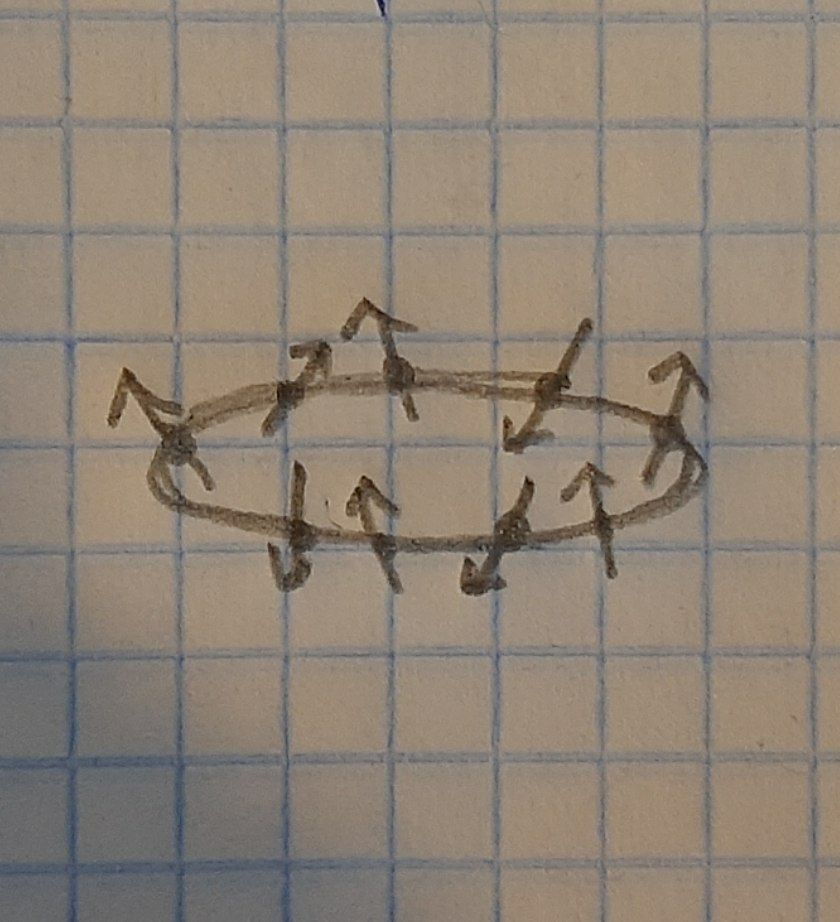
\includegraphics[width=0.5\linewidth]{chapter3/figures_special/isingchain1.jpg}
      \caption{Cadena de Ising abierta.}
    \end{subfigure}%
    \begin{subfigure}{0.5\textwidth}
      \centering
      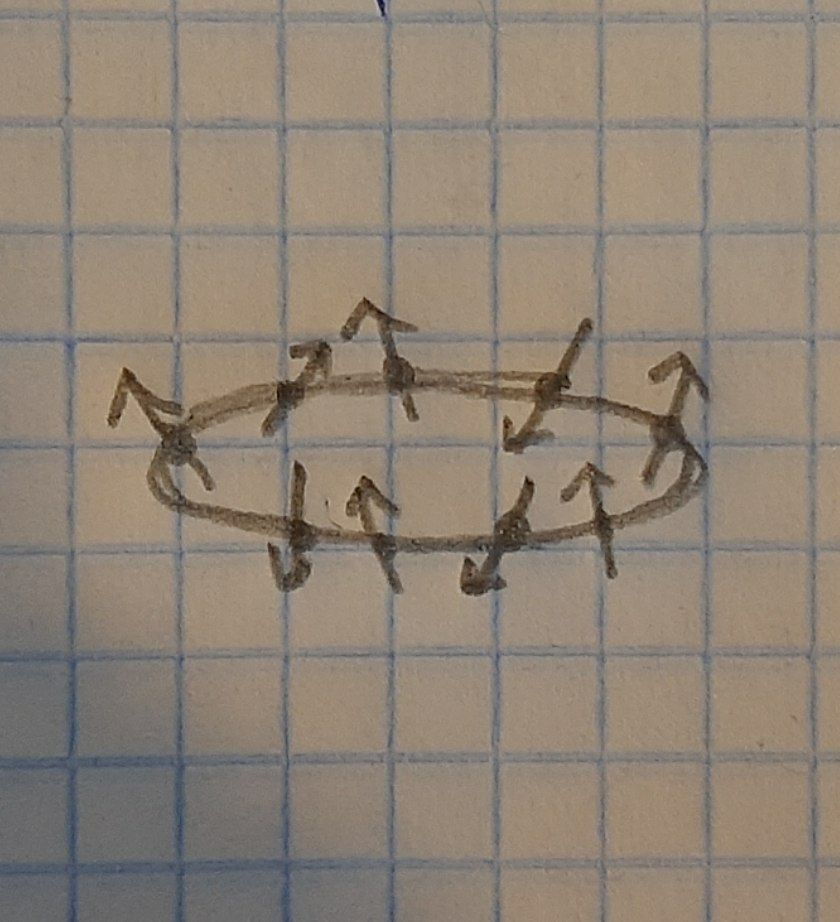
\includegraphics[width=0.5\linewidth]{chapter3/figures_special/isingchain1.jpg}
      \caption{Cadena de Ising cerrada}
    \end{subfigure}
    \label{fig:IsingChainOpenAndClosed}
\end{figure}
Sea entonces $\rho_{\ef}\in\densityspace{2}$ un estado efectivo correspondiente a un sistema de $n=2$ partículas, y $\varrho_{\max}$ el estado microscópico compatible con $\rho_{\ef}$ que maximiza la entropía. El hamiltoniano del sistema microscópico es, explícitamente,
\begin{equation}
    H=\omega\qty(\pauli{3}\otimes\pauli{3}),\nonumber
\end{equation}
de tal forma que dicho sistema evoluciona de acuerdo al operador unitario
\begin{equation}
    U=\Id \cos(\omega t)+ \rmi \pauli{3}\otimes\pauli{3} \sin(\omega t).\nonumber
\end{equation}
Si se propaga al estado de máxima entropía con dicho operador y se le pasa por la aplicación de grano grueso, la dinámica efectiva es
\begin{align}
    \Gamma_{t}(\rho_{\ef})=&\rho_{\ef} \cos^{2}(\omega)+\pauli{3} \rho_{\ef} \pauli{3} \sin^{2}(\omega t)\nonumber\\
    & + \rmi \sin(\omega t)\cos(\omega t)\qty(p_{1}\expval{\pauli{3}}_{2}[\pauli{3},\rho_{1}]+p_{2}\expval{\pauli{3}}_{1}[\pauli{3},\rho_{2}]).\nonumber
\end{align}
Dentro de la expresión de la dinámica efectiva reconocemos dos términos. El primero es un canal de desfasamiento sobre el estado efectivo, mientras que el segundo depende tanto de los parámetros de la aplicación de grano grueso, $p_{1}$ y $p_{2}$, como de valores esperados con respecto a los operadores de densidad reducidos del estado de máxima entropía. En efecto, el caso límite $p_{1}=1$ ve la dinámica efectiva reducida a un canal de desfasamiento en el tiempo,
\begin{equation}
    \Gamma_{t}(\rho_{\ef})=\rho_{\ef} \cos^{2}(\omega)+\pauli{3} \rho_{\ef} \pauli{3} \sin^{2}(\omega t).\nonumber
\end{equation}
mientras que el caso $p_{1}=p_{2}=\frac{1}{2}$ puede ser más informativo respecto al segundo término, pues en dicho caso
\begin{equation}
    \Gamma_{t}(\rho_{\ef})=\rho_{\ef} \cos^{2}(\omega)+\pauli{3} \rho_{\ef} \pauli{3} \sin^{2}(\omega t) + i\expval{\pauli{3}} \qty[\pauli{3},\rho_{\ef}] \sin(\omega t)\cos(\omega t).\nonumber
\end{equation}
Nótese que si $\expval{\pauli{3}}=1$, la dinámica es no solo lineal, sino unitaria, y corresponde a una rotación respecto al eje $z$, (con el detalle de que los estados tales que $\expval{\pauli{3}}=1$ son invariantes bajo dichas rotaciones). En realidad, el efecto de la dinámica efectiva sobre el estado es más clara en términos del vector de Bloch del estado inicial, $\vec{r}_{\ef}$.
\begin{equation}
    \Gamma_{t}(\vec{r}_{\ef})=\begin{pmatrix}
        x\cos(2\omega t)-yz\sin(2\omega t)\\
        xz\sin(2\omega t)+y\cos(2\omega t)\\
        z\\
    \end{pmatrix}.\nonumber
\end{equation}

La dinámica aplicada al vector de Bloch desplaza este en trayectoria elíptica centrada en el origen. A diferencia de una rotación circular, que tiene como único parámetro al ángulo de rotación, una rotación elíptica depende de los parámetros de la elipse, ambos semiejes y un argumento de rotación de la elipse, además del ángulo de rotación. En este caso, el vector de Bloch rota $2\omega t$ grados, a lo largo de la elipse de semieje mayor $\sqrt{1-z^2}$, semieje menor $z\sqrt{x^2+y^2}$ y argumento de rotación $\arccos(x)$. Esto es, los parámetros de la transformación dependen completamente del estado efectivo inicial. En este sentido, la dinámica es no lineal y no universal. La figura \ref{fig:Ising_p0.5_Sequence} presenta la evolución de la esfera de Bloch para el caso especial $p_{1}=\frac{1}{2}$.

\begin{figure}[ht!]
    \centering
    \begin{subfigure}{0.32\textwidth}
      \centering
      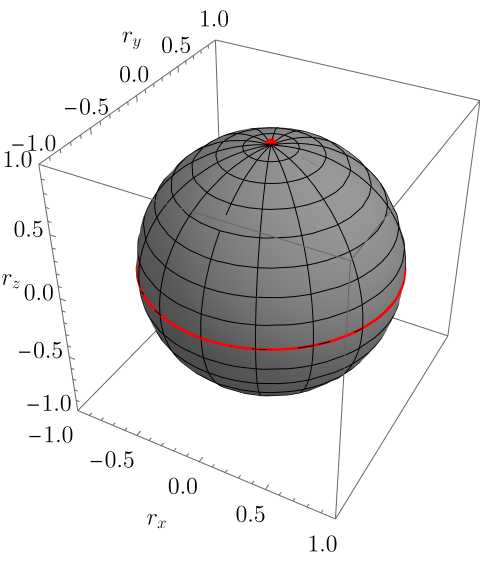
\includegraphics[width=0.9\linewidth]{chapter3/figures_special/sphere_Ising_t=0._z=0.9_p=0.5.png}
      \caption{$t=0$}
    \end{subfigure}%
    \begin{subfigure}{0.32\textwidth}
      \centering
      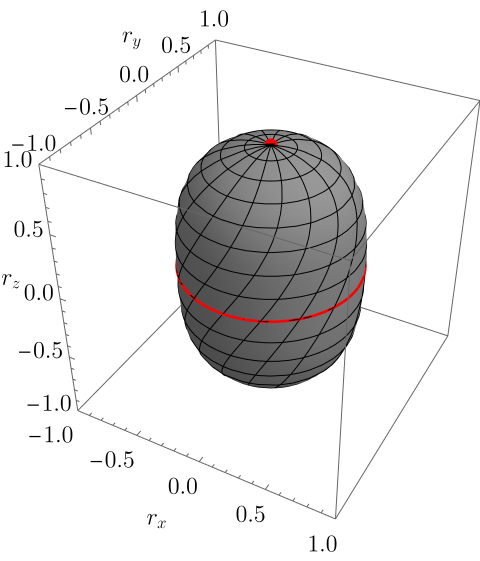
\includegraphics[width=0.9\linewidth]{chapter3/figures_special/sphere_Ising_t=0.5_z=0.9_p=0.5.png}
      \caption{$t=0.5$}
    \end{subfigure}
    \begin{subfigure}{0.32\textwidth}
      \centering
      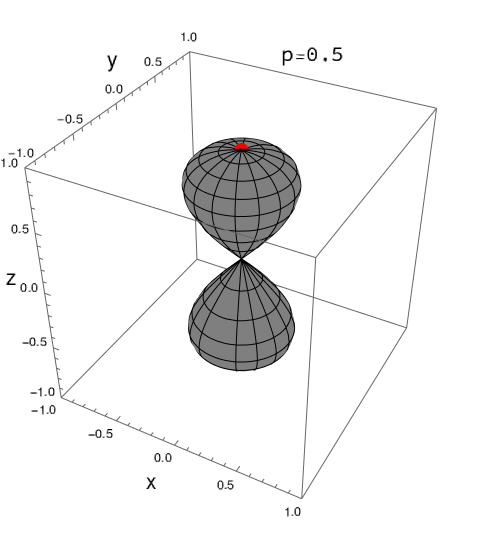
\includegraphics[width=0.9\linewidth]{chapter3/figures_special/sphere_Ising_t=1._z=0.9_p=0.5.png}
      \caption{$t=1$}
    \end{subfigure}
    \caption{Efecto del la evolución sobre la esfera de Bloch cuando $p=\frac{1}{2}$. Nótese que el desfasamiento sólo se completa en el eje $xy$.}
    \label{fig:Ising_p0.5_Sequence}
    \end{figure}

Como es natural, la expresión de la dinámica efectiva se vuelve cada vez más complicada y menos informativa conforme se aumenta el número de partículas. La dinámica unitaria general para la cadena de Ising cerrada sin campo transversal es
\begin{align}
    U=&\qty(\cos^{n}(\omega t)+(-\rmi)^{n}\sin^{n}(\omega t))\Id\nonumber\\ 
    &+\sum_{k=2}^{n-1}(-\rmi)^{n-k}\cos^{k}(\omega t)\sin^{n-k}(\omega t)\sum_{k_{1}<k_{2}}(\pauli{3,k_{1}}\pauli{3,k_{1}+1})(\pauli{3,k_{2}}\pauli{3,k_{2}+1}),\nonumber
\end{align}
mientras que para la cadena de Ising abierta es
\begin{align}
    U=&\cos^{n}(\omega t)\Id+(-\rmi)^{n}\sin^{n}(\omega t)\pauli{3,1}\pauli{3,n}\nonumber\\ 
    &+\sum_{k=2}^{n-1}(-\rmi)^{n-k}\cos^{k}(\omega t)\sin^{n-k}(\omega t)\sum_{k_{1}<k_{2}}(\pauli{3,k_{1}}\pauli{3,k_{1}+1})(\pauli{3,k_{2}}\pauli{3,k_{2}+1}).\nonumber
\end{align}
Si se quisiera hallar la dinámica efectiva, esta tendría términos dependientes de los valores esperados de todos los operadores $\pauli{3}^{\vec{j}}$ donde $\vec{j}$ tiene $n-1$ entradas, cosa que se traduce como un mínimo de $2^{n-1}$ términos. Aunque en este trabajo no se buscarán dichas expresiones, es posible usar calculadoras simbólicas para obtener visualizaciones de dichas dinámicas efectivas. Las figuras \ref{fig:Ising_n=3} a \ref{fig:Ising_n=8} muestran estas visualizaciones, mientras que las figuras \ref*{fig:Ising_n=3} a \ref{fig:Ising_n=8} muestran la trayectoria de diferentes vectores de Bloch efectivos bajo las mismas dinámicas.

\begin{figure}
    \centering
    \begin{subfigure}[b]{0.475\textwidth}
        \centering
        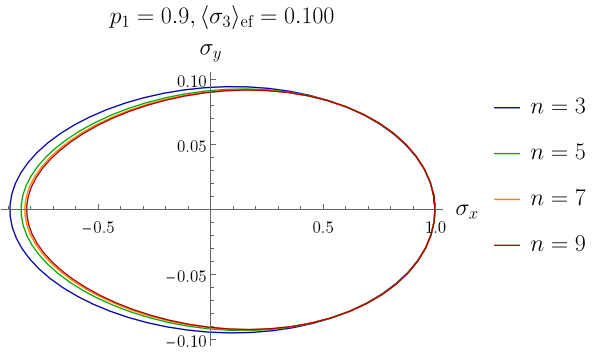
\includegraphics[width=\textwidth]{chapter3/figures_special/Ising_open_preferential_equal_p_n=n_r=1._z=0.10_p1=0.9.png}
        \caption{$p_{1}=0.9$}  
        \label{fig:OpenIsingPure1}
    \end{subfigure}
    \hfill
    \begin{subfigure}[b]{0.475\textwidth}  
        \centering 
        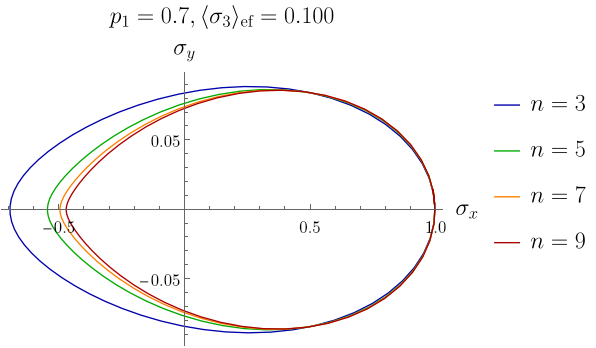
\includegraphics[width=\textwidth]{chapter3/figures_special/Ising_open_preferential_equal_p_n=n_r=1._z=0.10_p1=0.7.png}
        \caption{$p_{1}=0.7$}    
        \label{fig:OpenIsingPure2}
    \end{subfigure}
    \vskip\baselineskip
    \begin{subfigure}[b]{0.475\textwidth}   
        \centering 
        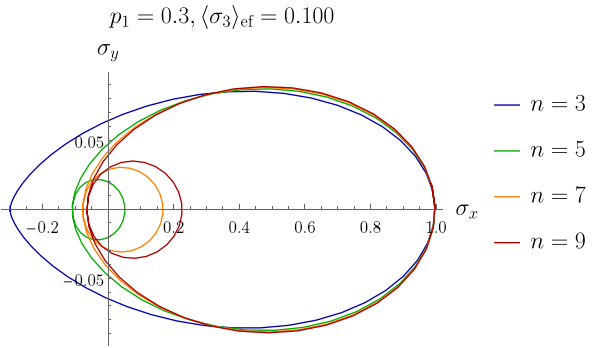
\includegraphics[width=\textwidth]{chapter3/figures_special/Ising_open_preferential_equal_p_n=n_r=1._z=0.10_p1=0.3.png}
        \caption{$p_{1}=0.3$}   
        \label{fig:OpenIsingPure3}
    \end{subfigure}
    \hfill
    \begin{subfigure}[b]{0.475\textwidth}   
        \centering 
        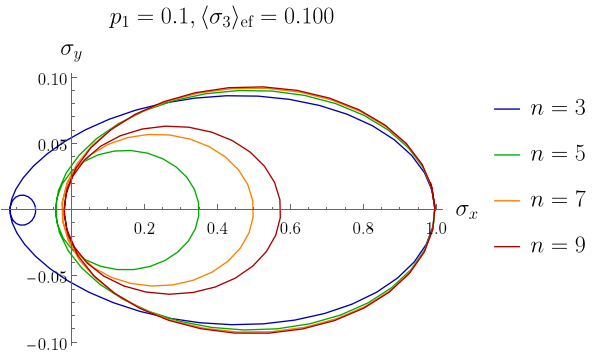
\includegraphics[width=\textwidth]{chapter3/figures_special/Ising_open_preferential_equal_p_n=n_r=1._z=0.10_p1=0.1.png}
        \caption{$p_{1}=0.1$}    
        \label{fig:OpenIsingPure4}
    \end{subfigure}
    \caption{Trayectorias del vector de Bloch de $\rho_{\ef}$ para si $r_{\ef}=1$ a una altura $z_{\ef}=0.1$, para diferentes valores de $n$ y $p_{1}$}
    \label{fig:OpenIsingPure}
\end{figure}

En general, los reusultados son no lineales. Se observa que, en los casos en los que se escoge $p_{k}=\frac{1}{n-1}\,\forall\,k\neq 1$, la evolución acerca más al estado efectivo hacia el desfasamiento. Para el caso en que las probabilidades diferentes a la de la primera partícula son aleatorias, los resultados son variados. El caso en que $p_{k}=\frac{1}{n-1}\,\forall\,k$. El caso en que el estado efectivo inicial es puro,
\acnote{hoy se me hizo algo tarde pero  tengo que obtener figuras como las que obtuve hoy para el caso puro y para el caso del Boltzman. Ya con eso se termina este capítulo.}

\acnote{agregar interpretación de los resultados numéricos}. Debido a que el tamaño de las matrices requeridas para el cálculo de la dinámica efectiva de un sistema microscópico de $n$ partículas aumenta como $2^{n}$, no fue posible obtener resultados numéricos para $n$ grande.



\newpage
\chapter{Conclusiones}

\ddnote{Comienza explicando que hiciste. Tipo: se estudió la dinámica emergente al combinar el principio de MaxEnt con un modelo de grano grueso, tal que en el nivel fino se cumple la mecánica cuántica. En particular se estudiaron los sistemas tales, presentados en el capitulo tal.}


\ddnote*{ideas buenas, pero muy cantinfleado, el párrafo es una sola frase también :S. No hay necesidad de ser extremadamente breves, explica con calma y separando en más oraciones}{Se estudió la dinámica efectiva que emergió de considerar un modelo de grano grueso que relaciona un estado efectivo de un qubit a un espacio microscópico de $n$ qubits, de utilizar el Principio de Máxima Entropía para hallar un estado fino compatible con dicho estado efectivo, y de asumir que el sistema microscópico evoluciona de acuerdo a las leyes de la mecánica cuántica.}

Se introdujo una aplicación de grano grueso que modela dos tipos de errores. El primero es el inducido por un aparato que tiene una probabilidad no nula de medir una partícula diferente a la pretendida. El segundo proviene de la incapacidad del detector de resolver todos los grados de libertad del sistema. Esta falta de resolución provoca que el sistema de $n$ qubits se vea como un sistema de uno solo. Se construyó una aplicación de asignación basada en el Principio de Máxima Entropía para hallar al estado microscópico menos sesgado posible, tal que fuera compatible con un estado efectivo dado. Asumiendo que el sistema fino evoluciona de manera que cumple con las leyes de la mecánica cuántica, se estudiaron las dinámicas efectivas inducidas por dichas evoluciones, el modelo de grano grueso y la aplicación de asignación.

\acnote{Arranca mejor la primera versión. La primera frase de un párrafo debe explicar el contenido del párrafo. El modelo de grano grueso no modela dos tipos de errores. El modelo de grano grueso surge de la concatenación de dos tipos de errores.}

Como se discutió en el capítulo \ref{sec:chapter2}, del modelo de grano grueso utilizado se reconocieron dos regímenes particularmente interesantes, \acnote{régimen imparical} \ddnote*{discutamos este nombre. Propongo algo como \textit{caso no sesgado}}{el régimen de Boltzmann}, asociado a una caja de $n$ partículas idénticas en la que cada una es igualmente probable de ser medida, y el régimen de partícula preferencial, en el que una partícula tiene una probabilidad mucho mayor de ser medida. En estos regímenes, la asignación de máxima entropía está dada por las ecuaciones (\ref{eq:BoltzmannAss}) y (\ref{eq:PreferentialAss}) respectivamente.

\ddnote*{De acuerdo a lo hallado en el capítulo \ref{sec:chapter3}, a través de la utilización de un modelo de grano grueso para estudiar la dinámica efectiva de sistemas de muchas partículas (ver ecuación tal (esas donde muestras la concatenación)), es posible hallar comportamientos más afines a la física clásica que a la mecánica cuántica, como la no linealidad de las evoluciones.}{De acuerdo a lo hallado en el capítulo \ref{sec:chapter3}, a través de la utilización de un modelo de grano grueso para estudiar la dinámica efectiva de sistemas de muchas partículas es posible hallar comportamientos más afines a la física clásica que a la mecánica cuántica, como la no linealidad de las evoluciones.} Sin embargo, las no linealidades encontradas, a diferencia de las dinámicas clásicas no lineales, no son universales. Esto debido a que todas resultaron dependientes del estado efectivo inicial. 
%
Otra diferencia viene del hecho que las evoluciones clásicas \ddnote{$deterministas$} no conllevan cambios en la entropía del sistema, mientras que las evoluciones efectivas estudiadas se traducían en contracciones de la esfera de Bloch, quizá mejor representadas por la compuerta SWAP efectiva, (\ref{eq:EffectiveSWAPt}). Dicho de otra forma, las dinámicas efectivas resultaron ser procesos irreversibles \ddnote*{, manifestado en el aumento de la entropía del sistema.}{con cambios en la entropía del sistema efectivo.}

Alguna de las dinámicas estudiadas, particularmente aquellas generadas por evoluciones subyacentes con fuertes simetrías, resultaron ser no solo lineales, sino canales cuánticos, como el caso de ciertos tipos de canales de Pauli, (\ref{eq:EffectiveDephasing}) y (\ref{eq:EffectiveDepolarizing}), y el canal de estabilización (\ref{eq:EffectiveStabilizing}), o aún más, evoluciones unitarias, como el caso de la dinámica local simétrica (\ref{eq:EffectiveSymmetricLocal}). 

Ninguna de las dinámicas estudiadas es no lineal en el caso en que las partículas no preferenciales tienen una probabilidad nula de ser detectadas, esto es, cuando el error es nulo, que equivale al caso en que la aplicación de medición borrosa sale del escenario. Aunque el único elemento no lineal en la composición que define a la dinámica efectiva es la aplicación de asignación, queda por investigar si es la aplicación de asignación o la aplicación de medición borrosa la causante de las no linealidades en las dinámicas efectivas.
\ddnote{Mañana hagamos un recuento de observaciones, para ver que mas ponemos aquí.}
\appendix
\chapter{Demostraciones de relaciones frecuentemente socorridas}

\subsubsection{Cuadrado de vector de pauli}
Se cumple que
\begin{align*}
    (\paulivec{r})(\paulivec{r})=&\sum_{j}r_{j}\pauli{j}\sum_{k}r_{k}\pauli{k}\\
    =&\sum_{j}r_{j}\sum_{k}r_{k}\pauli{j}\pauli{k}\\
    =&\sum_{j}r_{j}\sum_{k}r_{k}(\Id\delta_{jk}+i\epsilon_{jkl}\pauli{l})\\
    =&\sum_{j}r_{j}\sum_{k}r_{k}(\Id\delta_{jk})+i\sum_{j}r_{j}\sum_{k}r_{k}\epsilon_{jkl}\pauli{l})\\
    =&\Id
\end{align*}
Donde en la última línea se ha utilizado la antisimetría del tensor de Lévi-Civita. Se sigue que para todo entero positivo $p$
\begin{equation}\label{ap:PauliSquare}
    (\paulivec{n})^{2p}=\Id
\end{equation}

\subsubsection{Exponencial real de vector de Pauli}
Si se expande la serie de Taylor usando como argumento un vector de pauli $r\paulivec{r}$,
\begin{align*}
    e^{r\paulivec{r}}=&\sum_{k=0}^{\infty}\frac{1}{k!}(r\paulivec{r})^k\\
    =&\sum_{k}\frac{r^{2k}(\paulivec{r})^{2k}}{(2k)!}+\sum_{k}\frac{r^{2k+1}(\paulivec{r})^{2k+1}}{(2k+1)!},
\end{align*}
se puede usar (\ref{ap:PauliSquare}) para ver que
\begin{align*}
    e^{r\paulivec{r}}=&\Id\sum_{k}\frac{r^{2k}}{(2k)!}+\paulivec{r}\sum_{k}\frac{r^{2k+1}}{(2k+1)!},
\end{align*}
que, claro está, corresponde a
\begin{equation}\label{ap:PauliRealExp}
    e^{r\paulivec{r}}=\Id\cosh{r}+\paulivec{r}\sinh{r}
\end{equation}


\subsubsection{Exponencial compleja de un vector de Pauli}
Si se expande la serie de Taylor usando como argumento un vector de pauli $r\paulivec{r}$,
\begin{align*}
    e^{-ir\paulivec{r}}=&\sum_{k=0}^{\infty}\frac{1}{k!}(r\paulivec{r})^k\\
    =&\sum_{k}\frac{r^{2k}(\paulivec{r})^{2k}}{(2k)!}+\sum_{k}\frac{r^{2k+1}(\paulivec{r})^{2k+1}}{(2k+1)!},
\end{align*}
se puede usar (\ref{ap:PauliSquare}) para ver que
\begin{align*}
    e^{r\paulivec{r}}=&\Id\sum_{k}\frac{r^{2k}}{(2k)!}+\paulivec{r}\sum_{k}\frac{r^{2k+1}}{(2k+1)!},
\end{align*}
que, claro está, corresponde a
\begin{equation}\label{ap:PauliCompExp}
    e^{-ir\paulivec{r}}=\Id\cos{r}-i\paulivec{r}\sin{r}
\end{equation}
\subsubsection{Unitaria generada por un operador hermítico}
Toda unitaria de $2\times 2$ puede generarse a través de un operador hermítico $H$ como
\begin{equation*}
    U=e^{-iH}
\end{equation*}
Pues bien, como el conjunto de las matrices de Pauli, junto a la identidad, forman una base del espacio de operadores (respecto al producto interno de Hilbert-Schmidt), $H$ puede expandirse como $H=r_{0}\Id+r_{x}\pauli{x}+r_{y}+\pauli{y}+r_{z}\pauli{z}$. Si se utiliza este para construir una unitaria, desarrollando la serie se encuentra que
\begin{align*}
    e^{-iH}=&e^{-i(r_{0}\Id+r\paulivec{r})}\\
    =&e^{-i r_{0}\Id}e^{-ir\paulivec{r}}\\
    =&e^{-ir\paulivec{r}}\\
    =&\sum_{k=0}^{\infty}\frac{1}{k!}(-ir\paulivec{r})^k\\
    =&\sum_{k}(i)^{2k}(-1)^{2k}\frac{r^{2k}(\paulivec{r})^{2k}}{(2k)!}+\sum_{k}(i)^{2k+1}(-1)^{2k+1}\frac{r^{2k+1}(\paulivec{r})^{2k+1}}{(2k+1)!}\\
    =&-\Id\sum_{k}(-1)^{2k}\frac{r^{2k}}{(2k)!}-i(\paulivec{r})\sum_{k}(-1)^{2k}\frac{r^{2k+1}}{(2k+1)!}\\
    =&-\Id \cos{r}-i(\paulivec{r})\sin{r}
\end{align*}
\subsubsection{Vector de Pauli sobre vector de Pauli}
Si se aplica un vector de Pauli sobre otro se halla lo siguiente

\begin{align*}
    (\hat{n}\cdot\vec{\sigma})(\hat{m}\cdot\vec{\sigma})
\end{align*}

\subsubsection{Evolución de operador de densidad por operador unitario}
\begin{align*}
    e^{-i\omega t \paulivec{r}}\rho e^{i\omega t \paulivec{r}}=&(\Id \cos(\omega t)-i\paulivec{r} \sin(\omega t))\rho(\Id \cos(\omega t)+i\paulivec{r} \sin(\omega t))\\
    =&\rho\cos^{2}(\omega t)+(\paulivec{r})\rho(\paulivec{r})\sin^{2}(\omega t)+i\rho(\paulivec{r})\cos(\omega t)\sin(\omega t)-i(\paulivec{r})\rho \sin(\omega t)\cos(\omega t)\\
    =&\rho\cos^{2}(\omega t)+(\paulivec{r})\rho(\paulivec{r})\sin^{2}(\omega t)+i\sin(\omega t)\cos(\omega t)[\rho,\paulivec{r}]
\end{align*}
\chapter{Figuras}

\vspace*{-3in}

\begin{figure}
\vspace{2.4in}
\caption{Figura vacía}
\label{arm:fig1}
\end{figure}
\clearpage
\newpage

\begin{figure}
\vspace{2.4in}
\caption{Otra figura vacía}
\label{arm:fig2}
\end{figure}
\clearpage
\newpage

\chapter{La aplicación de asignación promedio}\label{sec:AVG}

En este apéndice se compararán, numéricamente \acnote{es numéricamente? porque aunque yo ya no hago más cálculos, esto usando expresiones halladas analíticamente}, las dinámicas efectivas obtenidas a través de la asignación de máxima entropía con otro tipo de asignación, con el objetivo de mostrar la dependencia fundamental de la dinámica en la aplicación de asignación y su naturaleza de estimación.

\section{Definición y acercamiento}




Nos interesamos en este apéndice en la \textit{asignación de aplicación promedio} \cite{Macro-To-Micro}. Esta aplicación asigna a un estado efectivo $\rho_{\ef} \in \densityspace{n}$ un estado microscópico $\varrho_{\avg} \in \densityspace{m}$ que es una mezcla estadística de estados finos. Más específicamente, le asigna el promedio del conjunto de todos los estados puros microscópicos tales que son compatibles con el estado efectivo bajo una aplicación de grano grueso en particular (en este trabajo, la dada por la ecuación \ref{eq:CG}). Dicho conjunto de estados puros microscópicos queda definido como
\begin{equation}\label{eq:Omega}
    \Omega_{\mcC}(\rho_{\ef}) = \{\ket{\psi}\in\hilbert_{m}:\, \mcC(\dyad{\psi}) = \rho_{\ef}  \}.
\end{equation}
La aplicación de asignación promedio es el promedio sobre dicho conjunto, \ie 
\begin{equation}\label{eq:AvgMap}
    \mcA_{\mcC}^{\avg}(\rho_{\ef}) = \overline{\Omega_{\mcC}(\rho_{\ef})} = \int d \mu\,\, \delta(\mcC(\dyad{\psi})-\rho_{\ef})\,\dyad{\psi},
\end{equation}
donde $d\mu$ es la medida de Haar sobre los estados puros de $\hilbert_{m}$. La delta de Dirac asegura que únicamente se tomen en consideración a los estados puros compatibles, y la medida de Haar, que la integración sobre dicho conjunto sea uniforme. Dicho de otra forma, la aplicación de asignación promedio asume dos cosas sobre el sistema microscópico: que puede estar estar en un estado puro, y que todos los estados puros son igualmente probables.

La solución analítica a la ecuación (\ref{eq:AvgMap}) ha sido encontrada para el caso en que la aplicación de grano grueso va de $\densityspace{4}$ a $\densityspace{2}$. Esto es, del espacio de dos partículas de dos niveles, al espacio de una partícula de dos niveles. En este trabajo no se profundizará en dicho resultado, pero se utilizará para poder comparar ambas aplicaciones de asignación.

\section{Diferencia entre el MaxEnt y el AssMap}

Aunque las hipótesis de la aplicación de asignación promedio puedan parecer razonables, Jaynes, en su artículo, argumenta que estas son tan arbitrarias como cualquier otra suposición, a menos que algún tipo de simetría del sistema sugiera lo contrario. Nos preguntamos, pues, sobre la diferencia entre el estado de máxima entropía y el estado promedio. Calculamos, pues, la distancia entre estos estados como una función del parámetro $p_{1}$ de la aplicación de grano grueso (recuérdese que en el caso $n=1$ el segundo parámetro es simplemente $1-p_{1}$). Esto es, nos interesa obtener
\begin{equation}
    \text{d}\qty(\avgass(\rho_{\ef}),\maxass(\rho_{\ef}))=\text{d}\qty(\avgass(\rho_{\ef}),\maxass(\rho_{\ef}))(p_{1}),\nonumber
\end{equation}

\begin{figure}[ht!]
    \centering
    \begin{subfigure}{0.5\textwidth}
      \centering
      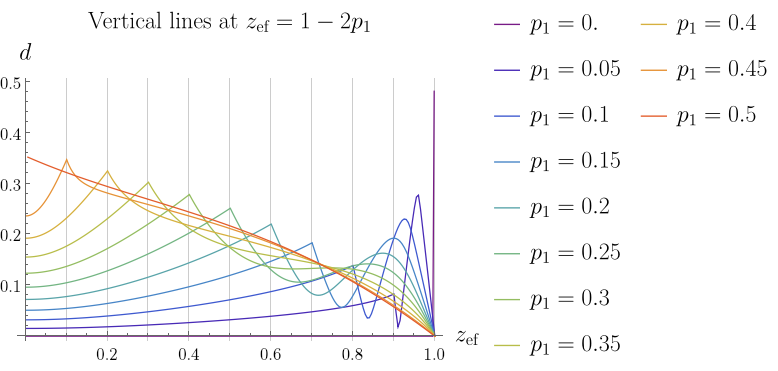
\includegraphics[width=0.9\linewidth]{appendices/figures/dist_avg_max_vs_z.png}
      \caption{Nueve no preferencial}
    \end{subfigure}%
    \begin{subfigure}{0.5\textwidth}
      \centering
      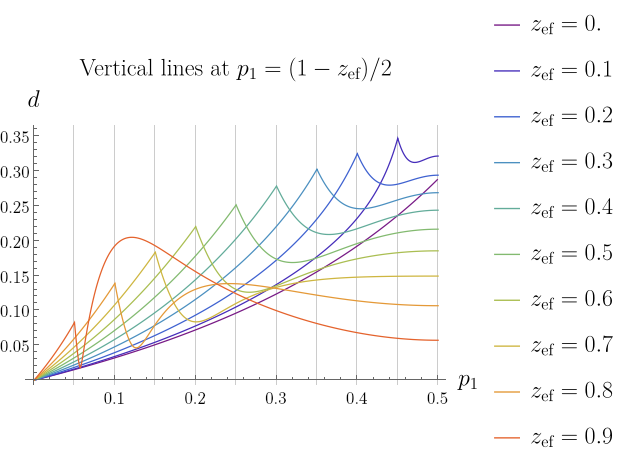
\includegraphics[width=0.9\linewidth]{appendices/figures/dist_avg_max_vs_p.png}
      \caption{Noventa y nueve partículas no preferenciales}
    \end{subfigure}
    \caption{Distancia entre asignaciones \acnote{Jjajaja tengo que arreglar esta figura}}\label{ap:DistAvgMaxEnt}
\end{figure}
La figura \ref{ap:DistAvgMaxEnt} revela que las asignaciones son iguales en el caso en el que $p_{1}=0$, así como cuando $r_{\ef}=1.$. En efecto, si el estado efectivo es puro, entonces \acnote{demostración de que son iguales}
\begin{align}
    lkjasdf
\end{align}
Además, se observan máximos locales en la distancia entre las asignaciones siempre que $p_{1}=\frac{1-r_{\ef}}{2}$. Esto es un resultado del comportamiento de la asignación promedio.

\section{Algunas dinámicas}

\subsection{Dinámicas factorizables}

\subsection{La compuerta SWAP}

\subsection{Canales de Pauli}

\section{Comparación de resultados de ambas asignaciones}
\bibliographystyle{ieeetr}
\bibliography{bibliography}
\end{document}
